\documentclass[11pt]{article}
\usepackage{amsmath,amssymb,array,booktabs,longtable,geometry,fontspec,xcolor}
\usepackage{tikz}\usetikzlibrary{arrows.meta}
\usepackage[hidelinks]{hyperref}
\definecolor{claimlink}{RGB}{25,70,150}
\newcommand{\pvar}[2]{\hyperlink{#1-P#2}{\textcolor{claimlink}{P_{#2}}}}
\newcommand{\pvartarget}[2]{\raisebox{\ht\strutbox}{\hypertarget{#1-P#2}{}}}
\makeatletter
\newenvironment{derivation}
  {\begin{list}{}{\setlength{\leftmargin}{2.6em}\setlength{\labelwidth}{2.2em}%
    \setlength{\labelsep}{0.4em}\setlength{\itemsep}{2pt}\setlength{\parsep}{0pt}%
    \setlength{\topsep}{6pt}\@beginparpenalty\@M\@itempenalty\@M%
    \interlinepenalty\@M\raggedright}}
  {\end{list}}
\newcommand{\breakrow}[1]{\@itempenalty\z@\item[#1]\@itempenalty\@M}
\newcommand{\keepwithnext}{\@endparpenalty\@M}
\makeatother
\clubpenalty=10000
\widowpenalty=10000
\newcommand{\gloss}[1]{\enspace---\enspace{\small\itshape #1}}
\geometry{margin=1in}
\setlength{\emergencystretch}{3em}
\frenchspacing
\IfFontExistsTF{Times New Roman}
  {\setmainfont{Times New Roman}[Ligatures=TeX]}
  {\IfFontExistsTF{FreeSerif}{\setmainfont{FreeSerif}[Ligatures=TeX]}{}}
\IfFontExistsTF{DejaVu Sans Mono}
  {\setmonofont{DejaVu Sans Mono}[Scale=MatchLowercase]}
  {\IfFontExistsTF{FreeMono}{\setmonofont{FreeMono}[Scale=MatchLowercase]}{}}
\title{The Triune God — what Scripture settles, and what it leaves open}
\author{\credit{TestimonyArguments.Trinity}}
\date{Generated by \texttt{lake exe argtex}}
\newcommand{\credit}[1]{\ifcsname credit@#1\endcsname\csname credit@#1\endcsname\fi}
\newcommand{\creditline}[1]{\ifcsname credit@#1\endcsname{\centering\credit{#1}\par\medskip}\fi}
\InputIfFileExists{credits.tex}{}{}
\begin{document}
\maketitle
\noindent This is one argument of the Testimony library, printed on its own. The library prints every argument together in \texttt{arguments.pdf}. This one is set as its Lean source sets it: the module docstrings as prose, in the order they are written, and under each one the package, line of reason, countermodel or result it introduces. Atoms are numbered propositional variables, numbered once per argument, so a variable means the same claim in every position within it; the legend gives each one's claim, its classification, the tradition that holds it and the source that carries it.

\noindent Nothing here asserts that the premises are true --- only that the conclusion does or does not follow from them.

\tableofcontents
\clearpage
\section*{The Triune God — what Scripture settles, and what it leaves open}
\addcontentsline{toc}{section}{The Triune God — what Scripture settles, and what it leaves open}

\subsection*{The Triune God: what Scripture settles, and what it leaves open}
\addcontentsline{toc}{subsection}{The Triune God: what Scripture settles, and what it leaves open}
Ken Kibbey’s \emph{Living Systematic Theology} (LST) is a systematic theology written in the open and revised whenever its author is persuaded that Scripture requires it. Its governing maxim is to speak “with the certainty Scripture gives, refusing certainty Scripture does not give”. So it grades its own claims: some it confesses as what Scripture establishes, some it defends as a synthesis Scripture “strongly grounds” without stating, and some it says are “not demonstrated”. Its section on the Triune God (§3, version 2.9, 21 October 2026) uses all three grades.

Those grades are claims about what follows from what, and that is what this library checks. A confessed claim should follow from the texts LST cites. A claim it calls not demonstrated should be \emph{independent} of them: neither it nor its denial should follow. This argument checks the grades, one question at a time, and reports what the checks find whichever way it goes.

\subsubsection*{The question encoded so far: does the Spirit proceed from the Son?}
The creed of the Council of Constantinople (381), the one Christians call the Nicene Creed, confesses that the Holy Spirit “proceeds from the Father”. In the West the words “and the Son” (\emph{Filioque}) were later added to it. The Council of Florence defined in 1439 “that the holy Spirit is eternally from the Father and the Son”, and the Westminster Confession confesses “the Holy Ghost eternally proceeding from the Father and the Son” (II.3). The Orthodox churches never accepted the addition. “Most Orthodox believe the Filioque to be theologically untrue,” Kallistos Ware writes. “They hold that the Spirit proceeds from the Father alone.”

LST once confessed the Filioque, as Westminster does. Version 2.9 says that it “no longer confesses” it, and gives its reasons:

\begin{quote}
These texts establish a real relation of the Spirit to both Father and Son. They do not state that the Spirit’s eternal origin is “from the Father and the Son” rather than “from the Father through the Son,” and they do not by themselves settle whether John 15:26 is speaking directly of eternal origin or of the Spirit’s mission. LST therefore no longer confesses the Western Filioque formula as a demonstrated biblical proposition.

\end{quote}
The chapter “Does the Spirit proceed from the Son?” checks each of those sentences, and each holds, with one limit. The texts establish the relation. They leave the Filioque open, and they also leave open whether John 15:26 speaks of eternal origin. The limit is that “through the Son” is not yet a position of its own, so what is checked is “and the Son” against “from the Father alone”. Each side needs at least one reading of its own beyond the texts. Any one of them is enough, so answering one does not answer the side. The chapter “Weighing the positions” sets LST, the West and the East against each other. What the texts establish is accepted however the disagreement is settled. The two sides defeat each other, so neither is.

\subsubsection*{The second question: is the Son less than the Father?}
LST also grades the texts of the Son’s obedience: “These texts establish real personal and mediatorial order, but they do not by themselves establish inequality of divine nature or an eternal hierarchy of command and obedience between the divine persons as such.” The chapter “Is the Son less than the Father?” checks that sentence, and it holds in each of its three parts. The texts establish an order of Father and Son in the work of salvation. They leave open whether the Son is less than the Father in his divinity, which the Arians read John 14:28 to say and Augustine, Athanasius and Calvin each answer differently. And they leave open whether the order is eternal, which Wayne Grudem and Bruce Ware hold and Kevin Giles denies. Weighed, what the texts establish is forced, and every reading beyond it stands off against another. That includes the Arian reading, which means only that these few verses do not settle the Son’s divinity. LST confesses it from other texts, the next question.

\subsubsection*{Still to come}
LST’s other graded claims in §3 are not yet encoded: that the Father, the Son and the Spirit are each God and are three persons, not three gods, against the Arians, the modalists and the “a god” of the New World Translation at John 1:1; and that eternal generation is a “defended synthesis” rather than a stated proposition. The issue that tracks this work lists them.

\subsection*{Is the Son less than the Father?}
\addcontentsline{toc}{subsection}{Is the Son less than the Father?}
Some texts set the Son below the Father. “The Son can do nothing of his own accord, but only what he sees the Father doing” (John 5:19). “The Father is greater than I” (John 14:28). The risen Jesus speaks of “my God and your God” (John 20:17). “The head of Christ is God” (1 Corinthians 11:3). And at the end “the Son himself will also be subjected to him who put all things in subjection under him” (1 Corinthians 15:28).

Ken Kibbey’s \emph{Living Systematic Theology} (LST) grades these texts so: “These texts establish real personal and mediatorial order, but they do not by themselves establish inequality of divine nature or an eternal hierarchy of command and obedience between the divine persons as such.” That is three claims, and all three hold. The texts establish an order of Father and Son in the work of salvation (\texttt{lst\allowbreak{}Order\_\allowbreak{}establishes}). They leave open whether the Son is less than the Father in his divinity (\texttt{order\_\allowbreak{}texts\_\allowbreak{}leave\_\allowbreak{}lesser\_\allowbreak{}divinity\_\allowbreak{}open}). And they leave open whether the order is eternal, an order of authority and submission between the persons as they are (\texttt{order\_\allowbreak{}texts\_\allowbreak{}leave\_\allowbreak{}eternal\_\allowbreak{}authority\_\allowbreak{}open}). LST calls the order “personal and mediatorial”. What is checked here is the order in the work of salvation, the mediatorial one; whether it also belongs to the persons as they eternally are is the third claim, and is left open.

\subsubsection*{Two questions, and who answers them}
The first question is the old one. The party that followed Arius (died 336) held the Son to be a creature, or unlike the Father, and read John 14:28 as saying so. The creed of Sirmium (357) says the Father is “greater in honour and dignity and Godhead … the Son Himself testifying, ‘The Father that sent Me is greater than I’”. Arius had written that “the Son has a beginning, but … God is without beginning”. Three readers answer the verse, and their answers differ.

\begin{itemize}
  \item Augustine reads it by the two “forms” of Philippians 2:6–7: “The Son of God, then, is equal to God the Father in nature, but less in fashion. For in the form of a servant which He took He is less than the Father; but in the form of God … He is equal to the Father.”
  \item Athanasius reads “greater” of the Father as the one the Son is from: “not indeed in greatness, nor in time, but because of His generation from the Father Himself, nay, in saying ‘greater’ He again shows that He is proper to His essence”, that is, belongs to the Father’s own being.
  \item Calvin reads it as Christ the Mediator, the one who stands between God and us (1 Timothy 2:5), comparing his humbled state with the glory he is going to: “Christ does not now speak either of his human nature, or of his eternal Divinity”. He calls the Fathers’ reading of the verse from the human nature “neither correct nor appropriate”. He holds the two forms; he denies that this verse speaks of them.
\end{itemize}
The second question was argued among evangelicals, most sharply at the Evangelical Theological Society in 2016, as “eternal functional subordination” or “eternal relations of authority and submission”. Wayne Grudem and Bruce Ware hold that the order of sending and obeying belongs to the persons as they eternally are: “the names Father and Son indicate an eternal relationship of authority and submission” (Grudem, 2016), and “prior to creation, the Son was eternally subject to the planning and authority of the Father” (Grudem, 2015, p. 40). Grudem confesses the persons “equal in power and glory”, with the Evangelical Theological Society, and holds that eternal submission does not deny it. Kevin Giles answers that “to argue that the Son is eternally subordinate in authority to the Father, denies that he is equal in power with the Father” (2008, p. 323). The Westminster Confession calls the three persons “of one substance, power, and eternity” (II.3). Millard Erickson, weighing the debate, holds that the texts of the Father’s sending and commanding “do not count as evidence in support of an eternal supremacy of the Father”; his words are quoted here as Grudem quotes them (2016), and Ware’s as Giles quotes them, since no page of either book was read.

\subsubsection*{The limits of what is checked}
The dispute hears the five order texts, Philippians 2:6, the Westminster Confession’s “power”, and four readings of John 14:28. It does not hear the texts that say the Son is God, John 1:1 and 20:28 among them, which are the next question of LST §3. So whatever it finds about the Son’s divinity is what those few verses carry, and no more.

\subsubsection*{How this is checked}
\paragraph*{The texts, and the order they establish}
\leavevmode\par\nobreak
\par\medskip\noindent\textbf{\texttt{order\allowbreak{}Texts}}\par\nobreak\noindent
The order texts LST cites.

\begin{derivation}
  \item[(1)] \(\pvar{TestimonyArguments.Trinity}{16}\)\gloss{John 5:19, 30 — the Son does nothing of his own accord, but the sender’s will}
  \item[(2)] \(\pvar{TestimonyArguments.Trinity}{17}\)\gloss{John 14:28 — “the Father is greater than I”}
  \item[(3)] \(\pvar{TestimonyArguments.Trinity}{18}\)\gloss{John 20:17 — the risen Jesus: “my God and your God”}
  \item[(4)] \(\pvar{TestimonyArguments.Trinity}{19}\)\gloss{1 Corinthians 11:3 — “the head of Christ is God”}
  \item[(5)] \(\pvar{TestimonyArguments.Trinity}{20}\)\gloss{1 Corinthians 15:28 — “the Son himself will also be subjected to him”}
\end{derivation}
\par\medskip\noindent\textbf{\texttt{texts\allowbreak{}Establish\allowbreak{}Order}}\par\nobreak\noindent
From the texts to a real order: the Son is sent and does the sender’s will, the Father is greater, the risen Son calls him his God, the head of Christ is God, and at the end the Son is subject.

\begin{derivation}
  \item[] \((\pvar{TestimonyArguments.Trinity}{16} \land \pvar{TestimonyArguments.Trinity}{17} \land \pvar{TestimonyArguments.Trinity}{18} \land \pvar{TestimonyArguments.Trinity}{19} \land \pvar{TestimonyArguments.Trinity}{20}) \rightarrow \pvar{TestimonyArguments.Trinity}{22}\)\gloss{\emph{would give:} There is a real order of Father and Son in the work of salvation}
\end{derivation}
\par\medskip\noindent\textbf{\texttt{order\allowbreak{}Line}} --- The order texts: the Son sent, obedient, and subject at the end\par\nobreak\noindent
\textbf{What the order texts establish}, on every party’s reading: a real order of Father and Son in the work of salvation.

\begin{derivation}
  \item[(1)] \(\pvar{TestimonyArguments.Trinity}{16}\)\gloss{John 5:19, 30 — the Son does nothing of his own accord, but the sender’s will}
  \item[(2)] \(\pvar{TestimonyArguments.Trinity}{17}\)\gloss{John 14:28 — “the Father is greater than I”}
  \item[(3)] \(\pvar{TestimonyArguments.Trinity}{18}\)\gloss{John 20:17 — the risen Jesus: “my God and your God”}
  \breakrow{(4)} \(\pvar{TestimonyArguments.Trinity}{19}\)\gloss{1 Corinthians 11:3 — “the head of Christ is God”}
  \breakrow{(5)} \(\pvar{TestimonyArguments.Trinity}{20}\)\gloss{1 Corinthians 15:28 — “the Son himself will also be subjected to him”}
  \item[(6)] \((\pvar{TestimonyArguments.Trinity}{16} \land \pvar{TestimonyArguments.Trinity}{17} \land \pvar{TestimonyArguments.Trinity}{18} \land \pvar{TestimonyArguments.Trinity}{19} \land \pvar{TestimonyArguments.Trinity}{20}) \rightarrow \pvar{TestimonyArguments.Trinity}{22}\)
  \item[\(\vdash\)] \(\pvar{TestimonyArguments.Trinity}{22}\)\gloss{\emph{at issue:} There is a real order of Father and Son in the work of salvation}
\end{derivation}
\par\medskip\noindent\textbf{\texttt{lst\allowbreak{}Order\allowbreak{}Case}} --- The order texts: the Son sent, obedient, and subject at the end\par\nobreak\noindent
\textbf{LST’s position on the order texts}: the texts, and the order they establish. Every premise is a text, cited to Scripture alone.

\begin{derivation}
  \item[(1)] \(\pvar{TestimonyArguments.Trinity}{16}\)\gloss{John 5:19, 30 — the Son does nothing of his own accord, but the sender’s will}
  \item[(2)] \(\pvar{TestimonyArguments.Trinity}{17}\)\gloss{John 14:28 — “the Father is greater than I”}
  \item[(3)] \(\pvar{TestimonyArguments.Trinity}{18}\)\gloss{John 20:17 — the risen Jesus: “my God and your God”}
  \breakrow{(4)} \(\pvar{TestimonyArguments.Trinity}{19}\)\gloss{1 Corinthians 11:3 — “the head of Christ is God”}
  \breakrow{(5)} \(\pvar{TestimonyArguments.Trinity}{20}\)\gloss{1 Corinthians 15:28 — “the Son himself will also be subjected to him”}
  \item[(6)] \((\pvar{TestimonyArguments.Trinity}{16} \land \pvar{TestimonyArguments.Trinity}{17} \land \pvar{TestimonyArguments.Trinity}{18} \land \pvar{TestimonyArguments.Trinity}{19} \land \pvar{TestimonyArguments.Trinity}{20}) \rightarrow \pvar{TestimonyArguments.Trinity}{22}\)
  \item[\(\vdash\)] \(\pvar{TestimonyArguments.Trinity}{22}\)\gloss{\emph{at issue:} There is a real order of Father and Son in the work of salvation}
  \keepwithnext
\end{derivation}
\emph{Grounded in scripture alone:} John 5:19, 30 — the Son does nothing of his own accord, but the sender’s will, John 14:28 — “the Father is greater than I”, John 20:17 — the risen Jesus: “my God and your God”, 1 Corinthians 11:3 — “the head of Christ is God”, 1 Corinthians 15:28 — “the Son himself will also be subjected to him”.
\paragraph*{Is the Son less in his divinity?}
\leavevmode\par\nobreak
\par\medskip\noindent\textbf{\texttt{greater\allowbreak{}To\allowbreak{}Lesser\allowbreak{}Divinity}}\par\nobreak\noindent
The Arian step: “greater” means lesser divinity.

\begin{derivation}
  \item[] \((\pvar{TestimonyArguments.Trinity}{17} \land \pvar{TestimonyArguments.Trinity}{23}) \rightarrow \pvar{TestimonyArguments.Trinity}{30}\)\gloss{\emph{would give:} The Son is less than the Father in his divinity}
\end{derivation}
\par\medskip\noindent\textbf{\texttt{arian\allowbreak{}Line}} --- “The Father is greater”: a lesser divinity (the Arians)\par\nobreak\noindent
\textbf{The Arian line}, as the creed of Sirmium (357) uses the verse, and as Augustine and Calvin report it.

\begin{derivation}
  \item[(1)] \(\pvar{TestimonyArguments.Trinity}{23}\)\gloss{In John 14:28 “greater” means the Son is less in his divinity}
  \item[(2)] \((\pvar{TestimonyArguments.Trinity}{17} \land \pvar{TestimonyArguments.Trinity}{23}) \rightarrow \pvar{TestimonyArguments.Trinity}{30}\)
  \item[\(\vdash\)] \(\pvar{TestimonyArguments.Trinity}{30}\)\gloss{\emph{at issue:} The Son is less than the Father in his divinity}
\end{derivation}
\par\medskip\noindent\textbf{\texttt{arian\allowbreak{}Case}} --- The Son less in divinity (the Arians)\par\nobreak\noindent
\textbf{The Arian position}: the order texts, and John 14:28 read as lesser divinity.

\begin{derivation}
  \item[(1)] \(\pvar{TestimonyArguments.Trinity}{16}\)\gloss{John 5:19, 30 — the Son does nothing of his own accord, but the sender’s will}
  \item[(2)] \(\pvar{TestimonyArguments.Trinity}{17}\)\gloss{John 14:28 — “the Father is greater than I”}
  \item[(3)] \(\pvar{TestimonyArguments.Trinity}{18}\)\gloss{John 20:17 — the risen Jesus: “my God and your God”}
  \breakrow{(4)} \(\pvar{TestimonyArguments.Trinity}{19}\)\gloss{1 Corinthians 11:3 — “the head of Christ is God”}
  \breakrow{(5)} \(\pvar{TestimonyArguments.Trinity}{20}\)\gloss{1 Corinthians 15:28 — “the Son himself will also be subjected to him”}
  \breakrow{(6)} \(\pvar{TestimonyArguments.Trinity}{23}\)\gloss{In John 14:28 “greater” means the Son is less in his divinity}
  \breakrow{(7)} \((\pvar{TestimonyArguments.Trinity}{16} \land \pvar{TestimonyArguments.Trinity}{17} \land \pvar{TestimonyArguments.Trinity}{18} \land \pvar{TestimonyArguments.Trinity}{19} \land \pvar{TestimonyArguments.Trinity}{20}) \rightarrow \pvar{TestimonyArguments.Trinity}{22}\)\gloss{\emph{would give:} There is a real order of Father and Son in the work of salvation}
  \item[(8)] \((\pvar{TestimonyArguments.Trinity}{17} \land \pvar{TestimonyArguments.Trinity}{23}) \rightarrow \pvar{TestimonyArguments.Trinity}{30}\)
  \item[\(\vdash\)] \(\pvar{TestimonyArguments.Trinity}{30}\)\gloss{\emph{at issue:} The Son is less than the Father in his divinity}
  \keepwithnext
\end{derivation}
\emph{Grounded in scripture alone:} John 5:19, 30 — the Son does nothing of his own accord, but the sender’s will, John 14:28 — “the Father is greater than I”, John 20:17 — the risen Jesus: “my God and your God”, 1 Corinthians 11:3 — “the head of Christ is God”, 1 Corinthians 15:28 — “the Son himself will also be subjected to him”.
\par\medskip\noindent\textbf{\texttt{two\allowbreak{}Forms\allowbreak{}To\allowbreak{}Equality}}\par\nobreak\noindent
Augustine’s step: less in the form of a servant, equal in the form of God.

\begin{derivation}
  \item[] \((\pvar{TestimonyArguments.Trinity}{17} \land \pvar{TestimonyArguments.Trinity}{21} \land \pvar{TestimonyArguments.Trinity}{24}) \rightarrow \lnot \pvar{TestimonyArguments.Trinity}{30}\)\gloss{\emph{would deny:} The Son is less than the Father in his divinity}
\end{derivation}
\par\medskip\noindent\textbf{\texttt{augustine\allowbreak{}Line}} --- Less in the form of a servant, equal in the form of God (Augustine)\par\nobreak\noindent
\textbf{Augustine’s line}, by the two forms.

\begin{derivation}
  \item[(1)] \(\pvar{TestimonyArguments.Trinity}{21}\)\gloss{Philippians 2:6 — “though he was in the form of God”}
  \item[(2)] \(\pvar{TestimonyArguments.Trinity}{24}\)\gloss{In John 14:28 the Son is less in the form of a servant, not in the form of God}
  \item[(3)] \((\pvar{TestimonyArguments.Trinity}{17} \land \pvar{TestimonyArguments.Trinity}{21} \land \pvar{TestimonyArguments.Trinity}{24}) \rightarrow \lnot \pvar{TestimonyArguments.Trinity}{30}\)
  \item[\(\vdash\)] \(\lnot \pvar{TestimonyArguments.Trinity}{30}\)\gloss{\emph{at issue, the denial of:} The Son is less than the Father in his divinity}
\end{derivation}
\par\medskip\noindent\textbf{\texttt{augustine\allowbreak{}Case}} --- Equal in nature, less in the form of a servant (Augustine)\par\nobreak\noindent
\textbf{Augustine’s position.}

\begin{derivation}
  \item[(1)] \(\pvar{TestimonyArguments.Trinity}{16}\)\gloss{John 5:19, 30 — the Son does nothing of his own accord, but the sender’s will}
  \item[(2)] \(\pvar{TestimonyArguments.Trinity}{17}\)\gloss{John 14:28 — “the Father is greater than I”}
  \item[(3)] \(\pvar{TestimonyArguments.Trinity}{18}\)\gloss{John 20:17 — the risen Jesus: “my God and your God”}
  \breakrow{(4)} \(\pvar{TestimonyArguments.Trinity}{19}\)\gloss{1 Corinthians 11:3 — “the head of Christ is God”}
  \breakrow{(5)} \(\pvar{TestimonyArguments.Trinity}{20}\)\gloss{1 Corinthians 15:28 — “the Son himself will also be subjected to him”}
  \breakrow{(6)} \(\pvar{TestimonyArguments.Trinity}{21}\)\gloss{Philippians 2:6 — “though he was in the form of God”}
  \breakrow{(7)} \(\pvar{TestimonyArguments.Trinity}{24}\)\gloss{In John 14:28 the Son is less in the form of a servant, not in the form of God}
  \breakrow{(8)} \((\pvar{TestimonyArguments.Trinity}{16} \land \pvar{TestimonyArguments.Trinity}{17} \land \pvar{TestimonyArguments.Trinity}{18} \land \pvar{TestimonyArguments.Trinity}{19} \land \pvar{TestimonyArguments.Trinity}{20}) \rightarrow \pvar{TestimonyArguments.Trinity}{22}\)\gloss{\emph{would give:} There is a real order of Father and Son in the work of salvation}
  \item[(9)] \((\pvar{TestimonyArguments.Trinity}{17} \land \pvar{TestimonyArguments.Trinity}{21} \land \pvar{TestimonyArguments.Trinity}{24}) \rightarrow \lnot \pvar{TestimonyArguments.Trinity}{30}\)
  \item[\(\vdash\)] \(\lnot \pvar{TestimonyArguments.Trinity}{30}\)\gloss{\emph{at issue, the denial of:} The Son is less than the Father in his divinity}
  \keepwithnext
\end{derivation}
\emph{Grounded in scripture alone:} John 5:19, 30 — the Son does nothing of his own accord, but the sender’s will, John 14:28 — “the Father is greater than I”, John 20:17 — the risen Jesus: “my God and your God”, 1 Corinthians 11:3 — “the head of Christ is God”, 1 Corinthians 15:28 — “the Son himself will also be subjected to him”, Philippians 2:6 — “though he was in the form of God”.
\par\medskip\noindent\textbf{\texttt{begetter\allowbreak{}To\allowbreak{}Equality}}\par\nobreak\noindent
Athanasius’s step: “greater” as the one the Son is from, so “proper to His essence”.

\begin{derivation}
  \item[] \((\pvar{TestimonyArguments.Trinity}{17} \land \pvar{TestimonyArguments.Trinity}{25}) \rightarrow \lnot \pvar{TestimonyArguments.Trinity}{30}\)\gloss{\emph{would deny:} The Son is less than the Father in his divinity}
\end{derivation}
\par\medskip\noindent\textbf{\texttt{athanasius\allowbreak{}Line}} --- Greater as the one he is from (Athanasius)\par\nobreak\noindent
\textbf{Athanasius’s line.}

\begin{derivation}
  \item[(1)] \(\pvar{TestimonyArguments.Trinity}{25}\)\gloss{The Father is “greater” as the one the Son is begotten from}
  \item[(2)] \((\pvar{TestimonyArguments.Trinity}{17} \land \pvar{TestimonyArguments.Trinity}{25}) \rightarrow \lnot \pvar{TestimonyArguments.Trinity}{30}\)
  \item[\(\vdash\)] \(\lnot \pvar{TestimonyArguments.Trinity}{30}\)\gloss{\emph{at issue, the denial of:} The Son is less than the Father in his divinity}
\end{derivation}
\par\medskip\noindent\textbf{\texttt{athanasius\allowbreak{}Case}} --- Greater as the one he is from (Athanasius)\par\nobreak\noindent
\textbf{Athanasius’s position.}

\begin{derivation}
  \item[(1)] \(\pvar{TestimonyArguments.Trinity}{16}\)\gloss{John 5:19, 30 — the Son does nothing of his own accord, but the sender’s will}
  \item[(2)] \(\pvar{TestimonyArguments.Trinity}{17}\)\gloss{John 14:28 — “the Father is greater than I”}
  \item[(3)] \(\pvar{TestimonyArguments.Trinity}{18}\)\gloss{John 20:17 — the risen Jesus: “my God and your God”}
  \breakrow{(4)} \(\pvar{TestimonyArguments.Trinity}{19}\)\gloss{1 Corinthians 11:3 — “the head of Christ is God”}
  \breakrow{(5)} \(\pvar{TestimonyArguments.Trinity}{20}\)\gloss{1 Corinthians 15:28 — “the Son himself will also be subjected to him”}
  \breakrow{(6)} \(\pvar{TestimonyArguments.Trinity}{25}\)\gloss{The Father is “greater” as the one the Son is begotten from}
  \breakrow{(7)} \((\pvar{TestimonyArguments.Trinity}{16} \land \pvar{TestimonyArguments.Trinity}{17} \land \pvar{TestimonyArguments.Trinity}{18} \land \pvar{TestimonyArguments.Trinity}{19} \land \pvar{TestimonyArguments.Trinity}{20}) \rightarrow \pvar{TestimonyArguments.Trinity}{22}\)\gloss{\emph{would give:} There is a real order of Father and Son in the work of salvation}
  \item[(8)] \((\pvar{TestimonyArguments.Trinity}{17} \land \pvar{TestimonyArguments.Trinity}{25}) \rightarrow \lnot \pvar{TestimonyArguments.Trinity}{30}\)
  \item[\(\vdash\)] \(\lnot \pvar{TestimonyArguments.Trinity}{30}\)\gloss{\emph{at issue, the denial of:} The Son is less than the Father in his divinity}
  \keepwithnext
\end{derivation}
\emph{Grounded in scripture alone:} John 5:19, 30 — the Son does nothing of his own accord, but the sender’s will, John 14:28 — “the Father is greater than I”, John 20:17 — the risen Jesus: “my God and your God”, 1 Corinthians 11:3 — “the head of Christ is God”, 1 Corinthians 15:28 — “the Son himself will also be subjected to him”.
\par\medskip\noindent\textbf{\texttt{mediators\allowbreak{}State\allowbreak{}Answers\allowbreak{}Arius}}\par\nobreak\noindent
Calvin’s step: the verse compares the Mediator’s state with his glory, so it does not say the Son is less in divinity.

\begin{derivation}
  \item[] \((\pvar{TestimonyArguments.Trinity}{17} \land \pvar{TestimonyArguments.Trinity}{26}) \rightarrow \lnot \pvar{TestimonyArguments.Trinity}{23}\)\gloss{\emph{would deny:} In John 14:28 “greater” means the Son is less in his divinity}
\end{derivation}
\par\medskip\noindent\textbf{\texttt{mediators\allowbreak{}State\allowbreak{}Answers\allowbreak{}The\allowbreak{}Fathers}}\par\nobreak\noindent
Calvin against the Fathers’ reply: the verse does not speak of the Son’s human nature either.

\begin{derivation}
  \item[] \(\pvar{TestimonyArguments.Trinity}{26} \rightarrow \lnot \pvar{TestimonyArguments.Trinity}{24}\)\gloss{\emph{would deny:} In John 14:28 the Son is less in the form of a servant, not in the form of God}
\end{derivation}
\par\medskip\noindent\textbf{\texttt{calvin\allowbreak{}Line}} --- The Mediator’s humbled state (Calvin)\par\nobreak\noindent
\textbf{Calvin’s line.}

\begin{derivation}
  \item[(1)] \(\pvar{TestimonyArguments.Trinity}{26}\)\gloss{In John 14:28 Christ compares his humbled state as Mediator with his glory}
  \item[(2)] \((\pvar{TestimonyArguments.Trinity}{17} \land \pvar{TestimonyArguments.Trinity}{26}) \rightarrow \lnot \pvar{TestimonyArguments.Trinity}{23}\)
  \item[\(\vdash\)] \(\lnot \pvar{TestimonyArguments.Trinity}{23}\)\gloss{\emph{at issue, the denial of:} In John 14:28 “greater” means the Son is less in his divinity}
\end{derivation}
\par\medskip\noindent\textbf{\texttt{calvin\allowbreak{}Case}} --- The Mediator’s state, not his natures (Calvin)\par\nobreak\noindent
\textbf{Calvin’s position}: John 14:28 does not say the Son is less in divinity, nor speak of his human nature.

\begin{derivation}
  \item[(1)] \(\pvar{TestimonyArguments.Trinity}{16}\)\gloss{John 5:19, 30 — the Son does nothing of his own accord, but the sender’s will}
  \item[(2)] \(\pvar{TestimonyArguments.Trinity}{17}\)\gloss{John 14:28 — “the Father is greater than I”}
  \item[(3)] \(\pvar{TestimonyArguments.Trinity}{18}\)\gloss{John 20:17 — the risen Jesus: “my God and your God”}
  \breakrow{(4)} \(\pvar{TestimonyArguments.Trinity}{19}\)\gloss{1 Corinthians 11:3 — “the head of Christ is God”}
  \breakrow{(5)} \(\pvar{TestimonyArguments.Trinity}{20}\)\gloss{1 Corinthians 15:28 — “the Son himself will also be subjected to him”}
  \breakrow{(6)} \(\pvar{TestimonyArguments.Trinity}{26}\)\gloss{In John 14:28 Christ compares his humbled state as Mediator with his glory}
  \breakrow{(7)} \((\pvar{TestimonyArguments.Trinity}{16} \land \pvar{TestimonyArguments.Trinity}{17} \land \pvar{TestimonyArguments.Trinity}{18} \land \pvar{TestimonyArguments.Trinity}{19} \land \pvar{TestimonyArguments.Trinity}{20}) \rightarrow \pvar{TestimonyArguments.Trinity}{22}\)\gloss{\emph{would give:} There is a real order of Father and Son in the work of salvation}
  \breakrow{(8)} \((\pvar{TestimonyArguments.Trinity}{17} \land \pvar{TestimonyArguments.Trinity}{26}) \rightarrow \lnot \pvar{TestimonyArguments.Trinity}{23}\)
  \item[(9)] \(\pvar{TestimonyArguments.Trinity}{26} \rightarrow \lnot \pvar{TestimonyArguments.Trinity}{24}\)\gloss{\emph{would deny:} In John 14:28 the Son is less in the form of a servant, not in the form of God}
  \item[\(\vdash\)] \(\lnot \pvar{TestimonyArguments.Trinity}{23}\)\gloss{\emph{at issue, the denial of:} In John 14:28 “greater” means the Son is less in his divinity}
  \keepwithnext
\end{derivation}
\emph{Grounded in scripture alone:} John 5:19, 30 — the Son does nothing of his own accord, but the sender’s will, John 14:28 — “the Father is greater than I”, John 20:17 — the risen Jesus: “my God and your God”, 1 Corinthians 11:3 — “the head of Christ is God”, 1 Corinthians 15:28 — “the Son himself will also be subjected to him”.
\paragraph*{Is the order eternal?}
\leavevmode\par\nobreak
\par\medskip\noindent\textbf{\texttt{order\allowbreak{}To\allowbreak{}Eternal\allowbreak{}Authority}}\par\nobreak\noindent
From the order, read as eternal, to an eternal relationship of authority and submission.

\begin{derivation}
  \item[] \((\pvar{TestimonyArguments.Trinity}{22} \land \pvar{TestimonyArguments.Trinity}{27}) \rightarrow \pvar{TestimonyArguments.Trinity}{31}\)\gloss{\emph{would give:} There is an eternal relationship of authority and submission of Father and Son}
\end{derivation}
\par\medskip\noindent\textbf{\texttt{eternal\allowbreak{}Order\allowbreak{}Line}} --- The order is eternal (Grudem, Ware)\par\nobreak\noindent
\textbf{The line of Grudem and Ware.}

\begin{derivation}
  \item[(1)] \(\pvar{TestimonyArguments.Trinity}{27}\)\gloss{The sending and obeying are the outworking of an eternal authority and submission}
  \item[(2)] \((\pvar{TestimonyArguments.Trinity}{22} \land \pvar{TestimonyArguments.Trinity}{27}) \rightarrow \pvar{TestimonyArguments.Trinity}{31}\)
  \item[\(\vdash\)] \(\pvar{TestimonyArguments.Trinity}{31}\)\gloss{\emph{at issue:} There is an eternal relationship of authority and submission of Father and Son}
\end{derivation}
\par\medskip\noindent\textbf{\texttt{eternal\allowbreak{}Authority\allowbreak{}Case}} --- Eternal authority and submission (Grudem, Ware)\par\nobreak\noindent
\textbf{The position of Grudem and Ware.}

\begin{derivation}
  \item[(1)] \(\pvar{TestimonyArguments.Trinity}{16}\)\gloss{John 5:19, 30 — the Son does nothing of his own accord, but the sender’s will}
  \item[(2)] \(\pvar{TestimonyArguments.Trinity}{17}\)\gloss{John 14:28 — “the Father is greater than I”}
  \item[(3)] \(\pvar{TestimonyArguments.Trinity}{18}\)\gloss{John 20:17 — the risen Jesus: “my God and your God”}
  \breakrow{(4)} \(\pvar{TestimonyArguments.Trinity}{19}\)\gloss{1 Corinthians 11:3 — “the head of Christ is God”}
  \breakrow{(5)} \(\pvar{TestimonyArguments.Trinity}{20}\)\gloss{1 Corinthians 15:28 — “the Son himself will also be subjected to him”}
  \breakrow{(6)} \(\pvar{TestimonyArguments.Trinity}{27}\)\gloss{The sending and obeying are the outworking of an eternal authority and submission}
  \breakrow{(7)} \((\pvar{TestimonyArguments.Trinity}{16} \land \pvar{TestimonyArguments.Trinity}{17} \land \pvar{TestimonyArguments.Trinity}{18} \land \pvar{TestimonyArguments.Trinity}{19} \land \pvar{TestimonyArguments.Trinity}{20}) \rightarrow \pvar{TestimonyArguments.Trinity}{22}\)\gloss{\emph{would give:} There is a real order of Father and Son in the work of salvation}
  \item[(8)] \((\pvar{TestimonyArguments.Trinity}{22} \land \pvar{TestimonyArguments.Trinity}{27}) \rightarrow \pvar{TestimonyArguments.Trinity}{31}\)
  \item[\(\vdash\)] \(\pvar{TestimonyArguments.Trinity}{31}\)\gloss{\emph{at issue:} There is an eternal relationship of authority and submission of Father and Son}
  \keepwithnext
\end{derivation}
\emph{Grounded in scripture alone:} John 5:19, 30 — the Son does nothing of his own accord, but the sender’s will, John 14:28 — “the Father is greater than I”, John 20:17 — the risen Jesus: “my God and your God”, 1 Corinthians 11:3 — “the head of Christ is God”, 1 Corinthians 15:28 — “the Son himself will also be subjected to him”.
\par\medskip\noindent\textbf{\texttt{equal\allowbreak{}Power\allowbreak{}Excludes\allowbreak{}Subordination}}\par\nobreak\noindent
From the Son’s equality in power, and eternal subordination’s denial of it, to no eternal subordination in authority.

\begin{derivation}
  \item[] \((\pvar{TestimonyArguments.Trinity}{28} \land \pvar{TestimonyArguments.Trinity}{29}) \rightarrow \lnot \pvar{TestimonyArguments.Trinity}{31}\)\gloss{\emph{would deny:} There is an eternal relationship of authority and submission of Father and Son}
\end{derivation}
\par\medskip\noindent\textbf{\texttt{equal\allowbreak{}Power\allowbreak{}Line}} --- Equal in power, so not eternally subordinate (Giles)\par\nobreak\noindent
\textbf{Giles’s line.}

\begin{derivation}
  \item[(1)] \(\pvar{TestimonyArguments.Trinity}{28}\)\gloss{The Son is equal to the Father in power: “of one substance, power, and eternity”}
  \item[(2)] \(\pvar{TestimonyArguments.Trinity}{29}\)\gloss{Eternal subordination in authority would deny the Son’s equality in power}
  \item[(3)] \((\pvar{TestimonyArguments.Trinity}{28} \land \pvar{TestimonyArguments.Trinity}{29}) \rightarrow \lnot \pvar{TestimonyArguments.Trinity}{31}\)
  \item[\(\vdash\)] \(\lnot \pvar{TestimonyArguments.Trinity}{31}\)\gloss{\emph{at issue, the denial of:} There is an eternal relationship of authority and submission of Father and Son}
\end{derivation}
\par\medskip\noindent\textbf{\texttt{equal\allowbreak{}Authority\allowbreak{}Case}} --- No eternal subordination in authority (Giles)\par\nobreak\noindent
\textbf{Giles’s position.}

\begin{derivation}
  \item[(1)] \(\pvar{TestimonyArguments.Trinity}{16}\)\gloss{John 5:19, 30 — the Son does nothing of his own accord, but the sender’s will}
  \item[(2)] \(\pvar{TestimonyArguments.Trinity}{17}\)\gloss{John 14:28 — “the Father is greater than I”}
  \item[(3)] \(\pvar{TestimonyArguments.Trinity}{18}\)\gloss{John 20:17 — the risen Jesus: “my God and your God”}
  \breakrow{(4)} \(\pvar{TestimonyArguments.Trinity}{19}\)\gloss{1 Corinthians 11:3 — “the head of Christ is God”}
  \breakrow{(5)} \(\pvar{TestimonyArguments.Trinity}{20}\)\gloss{1 Corinthians 15:28 — “the Son himself will also be subjected to him”}
  \breakrow{(6)} \(\pvar{TestimonyArguments.Trinity}{28}\)\gloss{The Son is equal to the Father in power: “of one substance, power, and eternity”}
  \breakrow{(7)} \(\pvar{TestimonyArguments.Trinity}{29}\)\gloss{Eternal subordination in authority would deny the Son’s equality in power}
  \breakrow{(8)} \((\pvar{TestimonyArguments.Trinity}{16} \land \pvar{TestimonyArguments.Trinity}{17} \land \pvar{TestimonyArguments.Trinity}{18} \land \pvar{TestimonyArguments.Trinity}{19} \land \pvar{TestimonyArguments.Trinity}{20}) \rightarrow \pvar{TestimonyArguments.Trinity}{22}\)\gloss{\emph{would give:} There is a real order of Father and Son in the work of salvation}
  \item[(9)] \((\pvar{TestimonyArguments.Trinity}{28} \land \pvar{TestimonyArguments.Trinity}{29}) \rightarrow \lnot \pvar{TestimonyArguments.Trinity}{31}\)
  \item[\(\vdash\)] \(\lnot \pvar{TestimonyArguments.Trinity}{31}\)\gloss{\emph{at issue, the denial of:} There is an eternal relationship of authority and submission of Father and Son}
  \keepwithnext
\end{derivation}
\emph{Grounded in scripture alone:} John 5:19, 30 — the Son does nothing of his own accord, but the sender’s will, John 14:28 — “the Father is greater than I”, John 20:17 — the risen Jesus: “my God and your God”, 1 Corinthians 11:3 — “the head of Christ is God”, 1 Corinthians 15:28 — “the Son himself will also be subjected to him”.
\paragraph*{Readings, written down}
\leavevmode\par\nobreak
\par\medskip\noindent\textbf{\texttt{nicen\allowbreak{}With\allowbreak{}Giles\allowbreak{}Reading}}\par\nobreak\noindent
\textbf{A Nicene reading with Giles}: every order text, the order, Augustine’s and Athanasius’s readings of John 14:28, the Son not less in divinity, the Son equal in power, and no eternal order of authority.

{\small\begin{verbatim}
def nicenWithGilesReading : Valuation Claim :=
  fun a =>
    match a with
    | Claim.greaterMeansLesserDivinity => False
    | Claim.sonLesserInDivinity => False
    | Claim.greaterAsMediatorsState => False
    | Claim.orderIsEternal => False
    | Claim.eternalAuthorityAndSubmission => False
    | x => True
\end{verbatim}}
\par\medskip\noindent\textbf{\texttt{arian\allowbreak{}Reading}}\par\nobreak\noindent
\textbf{The Arian reading}: every order text, the order, John 14:28 as lesser divinity, and the Son less in his divinity; none of the three Nicene readings of the verse.

{\small\begin{verbatim}
def arianReading : Valuation Claim :=
  fun a =>
    match a with
    | Claim.lessInTheFormOfAServant => False
    | Claim.greaterAsBegetter => False
    | Claim.greaterAsMediatorsState => False
    | x => True
\end{verbatim}}
\par\medskip\noindent\textbf{\texttt{augustine\allowbreak{}Reading}}\par\nobreak\noindent
\textbf{Augustine’s reading}: every order text, the order, the two forms, and the Son not less in divinity; not the Arian reading, and not Calvin’s, which denies that John 14:28 speaks of the two forms. It also makes the eternal order true. That is a choice of model, not Augustine’s answer to the second question.

{\small\begin{verbatim}
def augustineReading : Valuation Claim :=
  fun a =>
    match a with
    | Claim.greaterMeansLesserDivinity => False
    | Claim.sonLesserInDivinity => False
    | Claim.greaterAsMediatorsState => False
    | x => True
\end{verbatim}}
\par\medskip\noindent\textbf{\texttt{calvin\allowbreak{}Reading}}\par\nobreak\noindent
\textbf{Calvin’s reading}: every order text, the order, the Mediator’s state, and neither the Arian reading of John 14:28 nor Augustine’s reading of it by the two forms.

{\small\begin{verbatim}
def calvinReading : Valuation Claim :=
  fun a =>
    match a with
    | Claim.greaterMeansLesserDivinity => False
    | Claim.sonLesserInDivinity => False
    | Claim.lessInTheFormOfAServant => False
    | x => True
\end{verbatim}}
\par\medskip\noindent\textbf{\texttt{eternal\allowbreak{}Authority\allowbreak{}Reading}}\par\nobreak\noindent
\textbf{The reading of Grudem and Ware}: every order text, the order, the order read as eternal, and an eternal relationship of authority and submission. Giles’s reading, that such an order would deny the Son’s equal power, is not theirs.

{\small\begin{verbatim}
def eternalAuthorityReading : Valuation Claim :=
  fun a =>
    match a with
    | Claim.subordinationDeniesEqualPower => False
    | x => True
\end{verbatim}}
\par\medskip\noindent\textbf{\texttt{equal\allowbreak{}Authority\allowbreak{}Reading}}\par\nobreak\noindent
\textbf{Giles’s reading}: every order text, the order, the Son equal in power, and no eternal subordination in authority; the order not read as eternal.

{\small\begin{verbatim}
def equalAuthorityReading : Valuation Claim :=
  fun a =>
    match a with
    | Claim.orderIsEternal => False
    | Claim.eternalAuthorityAndSubmission => False
    | x => True
\end{verbatim}}
\paragraph*{What the order texts settle, and what they leave open}
\leavevmode\par\nobreak
\par\medskip\noindent\textbf{\texttt{lst\allowbreak{}Order\_\allowbreak{}establishes}}\par\nobreak\noindent
\textbf{Grant the order texts, and there is a real order of Father and Son.} This is what LST says they establish, and every party here grants it.

{\small\begin{verbatim}
theorem lstOrder_establishes : Establishes lstOrderCase
-- axioms: propext, Quot.sound
\end{verbatim}}
\par\medskip\noindent\textbf{\texttt{lst\allowbreak{}Order\allowbreak{}Case\_\allowbreak{}is\_\allowbreak{}satisfiable}}\par\nobreak\noindent
LST’s position on the order texts can be held without contradiction.

{\small\begin{verbatim}
theorem lstOrderCase_is_satisfiable : Satisfiable lstOrderCase.premises
-- axioms: propext, Quot.sound
\end{verbatim}}
\par\medskip\noindent\textbf{\texttt{order\_\allowbreak{}texts\_\allowbreak{}leave\_\allowbreak{}lesser\_\allowbreak{}divinity\_\allowbreak{}open}}\par\nobreak\noindent
\textbf{The order texts leave open whether the Son is less in his divinity.} Granted the five texts and the order they establish, neither “the Son is less than the Father in his divinity” nor its denial follows: the Arian reading satisfies every premise with it, and Augustine’s without it.

That is LST’s claim, and it holds. It is checked with each verse taken as its own words and each reading of it as a premise of its own. A reader who holds that “greater” plainly means greater in divinity puts that reading into the verse, and the reading is the premise rated \texttt{disputed}. Whether the Son is less in his divinity is argued from such readings, and from other texts, which the next question of LST §3 takes up.

{\small\begin{verbatim}
theorem order_texts_leave_lesser_divinity_open : Independent
    lstOrderCase.premises (p Claim.sonLesserInDivinity)
-- axioms: propext, Quot.sound
\end{verbatim}}
\par\medskip\noindent\textbf{\texttt{order\_\allowbreak{}texts\_\allowbreak{}leave\_\allowbreak{}eternal\_\allowbreak{}authority\_\allowbreak{}open}}\par\nobreak\noindent
\textbf{The order texts leave open whether the order is eternal.} Granted the texts and the order, neither an eternal relationship of authority and submission nor its denial follows: the reading of Grudem and Ware satisfies every premise with it, and Giles’s without it.

That is LST’s further claim, and it holds, checked in the same way: each verse as its own words, and the reading that the order is eternal as a premise of its own. Grudem argues that the subjection of 1 Corinthians 15:28 and the Son’s being sent from before creation already show it; that argument is the reading, rated \texttt{disputed}. Erickson draws LST’s conclusion about the texts of sending and commanding, that “they do not count as evidence in support of an eternal supremacy of the Father” (as Grudem quotes him).

{\small\begin{verbatim}
theorem order_texts_leave_eternal_authority_open : Independent
    lstOrderCase.premises (p Claim.eternalAuthorityAndSubmission)
-- axioms: propext, Quot.sound
\end{verbatim}}
\paragraph*{What each position delivers}
\leavevmode\par\nobreak
\par\medskip\noindent\textbf{\texttt{arian\allowbreak{}Case\_\allowbreak{}establishes}}\par\nobreak\noindent
\textbf{Grant John 14:28 read as lesser divinity, and the Son is less than the Father in his divinity.}

{\small\begin{verbatim}
theorem arianCase_establishes : Establishes arianCase
-- axioms: propext, Quot.sound
\end{verbatim}}
\par\medskip\noindent\textbf{\texttt{arian\allowbreak{}Case\_\allowbreak{}is\_\allowbreak{}satisfiable}}\par\nobreak\noindent
The Arian position can be held without contradiction.

{\small\begin{verbatim}
theorem arianCase_is_satisfiable : Satisfiable arianCase.premises
-- axioms: propext, Quot.sound
\end{verbatim}}
\par\medskip\noindent\textbf{\texttt{augustine\allowbreak{}Case\_\allowbreak{}establishes}}\par\nobreak\noindent
\textbf{Grant Augustine’s two forms, and the Son is not less in his divinity.}

{\small\begin{verbatim}
theorem augustineCase_establishes : Establishes augustineCase
-- axioms: propext, Quot.sound
\end{verbatim}}
\par\medskip\noindent\textbf{\texttt{augustine\allowbreak{}Case\_\allowbreak{}is\_\allowbreak{}satisfiable}}\par\nobreak\noindent
Augustine’s position can be held without contradiction.

{\small\begin{verbatim}
theorem augustineCase_is_satisfiable : Satisfiable augustineCase.premises
-- axioms: propext, Quot.sound
\end{verbatim}}
\par\medskip\noindent\textbf{\texttt{athanasius\allowbreak{}Case\_\allowbreak{}establishes}}\par\nobreak\noindent
\textbf{Grant Athanasius’s reading of “greater”, and the Son is not less in his divinity.}

{\small\begin{verbatim}
theorem athanasiusCase_establishes : Establishes athanasiusCase
-- axioms: propext, Quot.sound
\end{verbatim}}
\par\medskip\noindent\textbf{\texttt{athanasius\allowbreak{}Case\_\allowbreak{}is\_\allowbreak{}satisfiable}}\par\nobreak\noindent
Athanasius’s position can be held without contradiction.

{\small\begin{verbatim}
theorem athanasiusCase_is_satisfiable : Satisfiable athanasiusCase.premises
-- axioms: propext, Quot.sound
\end{verbatim}}
\par\medskip\noindent\textbf{\texttt{calvin\allowbreak{}Case\_\allowbreak{}establishes}}\par\nobreak\noindent
\textbf{Grant Calvin’s reading, and John 14:28 does not say the Son is less in his divinity.}

{\small\begin{verbatim}
theorem calvinCase_establishes : Establishes calvinCase
-- axioms: propext, Quot.sound
\end{verbatim}}
\par\medskip\noindent\textbf{\texttt{calvin\allowbreak{}Case\_\allowbreak{}is\_\allowbreak{}satisfiable}}\par\nobreak\noindent
Calvin’s position can be held without contradiction.

{\small\begin{verbatim}
theorem calvinCase_is_satisfiable : Satisfiable calvinCase.premises
-- axioms: propext, Quot.sound
\end{verbatim}}
\par\medskip\noindent\textbf{\texttt{eternal\allowbreak{}Authority\allowbreak{}Case\_\allowbreak{}establishes}}\par\nobreak\noindent
\textbf{Grant the order read as eternal, and there is an eternal relationship of authority and submission.}

{\small\begin{verbatim}
theorem eternalAuthorityCase_establishes : Establishes eternalAuthorityCase
-- axioms: propext, Quot.sound
\end{verbatim}}
\par\medskip\noindent\textbf{\texttt{eternal\allowbreak{}Authority\allowbreak{}Case\_\allowbreak{}is\_\allowbreak{}satisfiable}}\par\nobreak\noindent
The position of Grudem and Ware can be held without contradiction.

{\small\begin{verbatim}
theorem eternalAuthorityCase_is_satisfiable : Satisfiable
    eternalAuthorityCase.premises
-- axioms: propext, Quot.sound
\end{verbatim}}
\par\medskip\noindent\textbf{\texttt{equal\allowbreak{}Authority\allowbreak{}Case\_\allowbreak{}establishes}}\par\nobreak\noindent
\textbf{Grant the Son equal in power, and that eternal subordination would deny it, and there is no eternal subordination in authority.}

{\small\begin{verbatim}
theorem equalAuthorityCase_establishes : Establishes equalAuthorityCase
-- axioms: propext, Quot.sound
\end{verbatim}}
\par\medskip\noindent\textbf{\texttt{equal\allowbreak{}Authority\allowbreak{}Case\_\allowbreak{}is\_\allowbreak{}satisfiable}}\par\nobreak\noindent
Giles’s position can be held without contradiction.

{\small\begin{verbatim}
theorem equalAuthorityCase_is_satisfiable : Satisfiable
    equalAuthorityCase.premises
-- axioms: propext, Quot.sound
\end{verbatim}}
\subsection*{Weighing the readings of the order texts}
\addcontentsline{toc}{subsection}{Weighing the readings of the order texts}
Seven positions are parties to one dispute: LST, which holds only the order the texts establish; the Arians; Augustine, Athanasius and Calvin, each with his own reading of “the Father is greater than I”; Grudem and Ware, for an eternal order of authority and submission; and Giles, against it.

\subsubsection*{How to read the verdicts}
One position \emph{defeats} another when it denies something the other needs and does not rest on anything rated lower. Every reading here is rated \texttt{disputed}, the lowest rating, because cited readers disagree over it; so when two readings deny each other, each defeats the other, and that is a tie. A position is \emph{forced} when it is accepted however the ties are settled. It \emph{can be defended} when some consistent way of settling them accepts it, and it is \emph{not forced} when another consistent way leaves it out. Every defeat is computed from the positions’ premises, and Lean checks each computation.

\subsubsection*{What the weighing found}
LST’s position is accepted at once, because nothing defeats it (\texttt{the\_\allowbreak{}order\_\allowbreak{}prevails}): every other party holds every premise it holds.

Over the Son’s divinity, the Arian reading and each Nicene reading of John 14:28 (Nicene: of the Council of Nicaea, 325, which confessed the Son of one being with the Father) defeat each other. Calvin’s reading and Augustine’s defeat each other too, because Calvin denies that the verse speaks of the Son’s human nature. Every one of these positions can be defended and none is forced, the Arian one included (\texttt{arian\_\allowbreak{}reading\_\allowbreak{}defensible}, \texttt{arian\_\allowbreak{}reading\_\allowbreak{}not\_\allowbreak{}forced}, \texttt{augustine\_\allowbreak{}reading\_\allowbreak{}not\_\allowbreak{}forced}, \texttt{athanasius\_\allowbreak{}reading\_\allowbreak{}not\_\allowbreak{}forced}, \texttt{calvin\_\allowbreak{}reading\_\allowbreak{}not\_\allowbreak{}forced}). That is because the readings that answer the Arian one are rated no higher than it. It is a finding about the five order texts, Philippians 2:6 and four readings of one verse. LST confesses the Son’s divinity from John 1:1, 20:28 and the other texts of its next question, which this dispute does not hear.

Over the eternal order, Grudem and Ware and Giles defeat each other, and neither is forced (\texttt{eternal\_\allowbreak{}order\_\allowbreak{}not\_\allowbreak{}forced}, \texttt{equal\_\allowbreak{}authority\_\allowbreak{}not\_\allowbreak{}forced}). That agrees with LST: the texts do not establish an eternal hierarchy. If either reading were rated above the other, the verdict could change.

\subsubsection*{How this is checked}
\par\medskip\noindent\textbf{\texttt{order\allowbreak{}Party\allowbreak{}Node}}\par\nobreak\noindent
The package each party argues from.

{\small\begin{verbatim}
def orderPartyNode : OrderParty → ArgumentPackage Claim :=
  fun x =>
    match x with
    | OrderParty.lst => lstOrderCase
    | OrderParty.arian => arianCase
    | OrderParty.augustine => augustineCase
    | OrderParty.athanasius => athanasiusCase
    | OrderParty.calvin => calvinCase
    | OrderParty.eternal => eternalAuthorityCase
    | OrderParty.equal => equalAuthorityCase
\end{verbatim}}
\par\medskip\noindent\textbf{\texttt{order\allowbreak{}Dispute}}\par\nobreak\noindent
The dispute over the order texts: every party can be held without contradiction, delivers its conclusion, and has its steps rated.

{\small\begin{verbatim}
def orderDispute : Dispute Claim OrderParty :=
  { node := orderPartyNode, consistent := orderDispute._proof_1,
    sound := orderDispute._proof_2,
    rated := orderDispute._proof_10 }
\end{verbatim}}
\par\medskip\noindent\textbf{\texttt{order\allowbreak{}Dispute\_\allowbreak{}defeats}}\par\nobreak\noindent
\textbf{Who defeats whom}, all 49 pairs. The Arians and each of Augustine, Athanasius and Calvin defeat each other. Calvin and Augustine defeat each other as well: Calvin denies that John 14:28 speaks of the Son’s human nature, which is Augustine’s reading. Grudem and Ware and Giles defeat each other. Nothing attacks LST. Every cell is checked by the kernel.

{\small\begin{verbatim}
theorem orderDispute_defeats : ∀ (i j : OrderParty), orderDispute.defeats i j
    ↔ (i, j) ∈ [(OrderParty.arian, OrderParty.augustine),
    (OrderParty.augustine, OrderParty.arian), (OrderParty.arian,
    OrderParty.athanasius), (OrderParty.athanasius, OrderParty.arian),
    (OrderParty.arian, OrderParty.calvin), (OrderParty.calvin,
    OrderParty.arian), (OrderParty.augustine, OrderParty.calvin),
    (OrderParty.calvin, OrderParty.augustine), (OrderParty.eternal,
    OrderParty.equal), (OrderParty.equal, OrderParty.eternal)]
-- axioms: propext, Classical.choice, Quot.sound
\end{verbatim}}
\par\medskip\noindent\textbf{\texttt{order\allowbreak{}Dispute\_\allowbreak{}supports}}\par\nobreak\noindent
\textbf{Nothing supports anything}, in all 49 pairs. Every cell is checked by the kernel.

{\small\begin{verbatim}
theorem orderDispute_supports : ∀ (i j : OrderParty), ¬orderDispute.supports i
    j
-- axioms: propext, Classical.choice, Quot.sound
\end{verbatim}}
\par\medskip\noindent\textbf{\texttt{order\allowbreak{}Dispute\_\allowbreak{}part\allowbreak{}Of}}\par\nobreak\noindent
\textbf{LST’s case is part of every other party’s}, since each holds the order texts and the order drawn from them. Every cell is checked by the kernel.

{\small\begin{verbatim}
theorem orderDispute_partOf : ∀ (i j : OrderParty), orderDispute.partOf i j ↔
    i = j ∨ (i, j) ∈ [(OrderParty.lst, OrderParty.arian), (OrderParty.lst,
    OrderParty.augustine), (OrderParty.lst, OrderParty.athanasius),
    (OrderParty.lst, OrderParty.calvin), (OrderParty.lst, OrderParty.eternal),
    (OrderParty.lst, OrderParty.equal)]
-- axioms: propext, Classical.choice, Quot.sound
\end{verbatim}}
\par\medskip\noindent\textbf{\texttt{order\allowbreak{}Map}}\par\nobreak\noindent
The dispute over the order texts drawn: who defeats whom, and whose case is part of whose.

\begin{center}
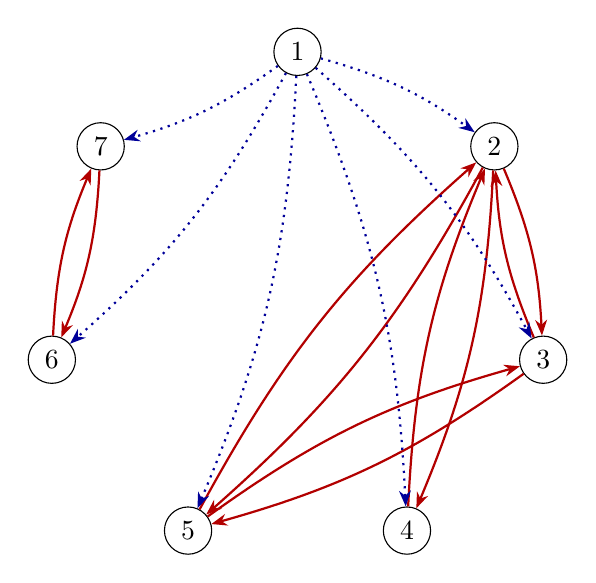
\begin{tikzpicture}[>={Stealth[length=2mm]}]
\node[draw,circle,minimum size=6mm,inner sep=0pt] (n0) at (0.00,3.20) {1};
\node[draw,circle,minimum size=6mm,inner sep=0pt] (n1) at (2.50,2.00) {2};
\node[draw,circle,minimum size=6mm,inner sep=0pt] (n2) at (3.12,-0.71) {3};
\node[draw,circle,minimum size=6mm,inner sep=0pt] (n3) at (1.39,-2.88) {4};
\node[draw,circle,minimum size=6mm,inner sep=0pt] (n4) at (-1.39,-2.88) {5};
\node[draw,circle,minimum size=6mm,inner sep=0pt] (n5) at (-3.12,-0.71) {6};
\node[draw,circle,minimum size=6mm,inner sep=0pt] (n6) at (-2.50,2.00) {7};
\draw[->,red!70!black,thick] (n1) to[bend left=10] (n2);
\draw[->,red!70!black,thick] (n1) to[bend left=10] (n3);
\draw[->,red!70!black,thick] (n1) to[bend left=10] (n4);
\draw[->,red!70!black,thick] (n2) to[bend left=10] (n1);
\draw[->,red!70!black,thick] (n2) to[bend left=10] (n4);
\draw[->,red!70!black,thick] (n3) to[bend left=10] (n1);
\draw[->,red!70!black,thick] (n4) to[bend left=10] (n1);
\draw[->,red!70!black,thick] (n4) to[bend left=10] (n2);
\draw[->,red!70!black,thick] (n5) to[bend left=10] (n6);
\draw[->,red!70!black,thick] (n6) to[bend left=10] (n5);
\draw[->,blue!60!black,thick,dotted] (n0) to[bend left=10] (n1);
\draw[->,blue!60!black,thick,dotted] (n0) to[bend left=10] (n2);
\draw[->,blue!60!black,thick,dotted] (n0) to[bend left=10] (n3);
\draw[->,blue!60!black,thick,dotted] (n0) to[bend left=10] (n4);
\draw[->,blue!60!black,thick,dotted] (n0) to[bend left=10] (n5);
\draw[->,blue!60!black,thick,dotted] (n0) to[bend left=10] (n6);
\end{tikzpicture}
\end{center}
\noindent Solid: defeats. Dashed: supports. Dotted: one party's case is part of another's.
\begin{enumerate}
\item The order texts: the Son sent, obedient, and subject at the end
\item The Son less in divinity (the Arians)
\item Equal in nature, less in the form of a servant (Augustine)
\item Greater as the one he is from (Athanasius)
\item The Mediator’s state, not his natures (Calvin)
\item Eternal authority and submission (Grudem, Ware)
\item No eternal subordination in authority (Giles)
\end{enumerate}
\begin{longtable}{@{}>{\raggedright\arraybackslash}p{0.3\textwidth} >{\raggedright\arraybackslash}p{0.3\textwidth} >{\raggedright\arraybackslash}p{0.3\textwidth}@{}}
\toprule
\textbf{From} & \textbf{To} & \textbf{Edge} \\
\midrule
\endhead
2 \emph{The Son less in divinity (the Arians)} & 3 \emph{Equal in nature, less in the form of a servant (Augustine)} & defeats \\
2 \emph{The Son less in divinity (the Arians)} & 4 \emph{Greater as the one he is from (Athanasius)} & defeats \\
2 \emph{The Son less in divinity (the Arians)} & 5 \emph{The Mediator’s state, not his natures (Calvin)} & defeats \\
3 \emph{Equal in nature, less in the form of a servant (Augustine)} & 2 \emph{The Son less in divinity (the Arians)} & defeats \\
3 \emph{Equal in nature, less in the form of a servant (Augustine)} & 5 \emph{The Mediator’s state, not his natures (Calvin)} & defeats \\
4 \emph{Greater as the one he is from (Athanasius)} & 2 \emph{The Son less in divinity (the Arians)} & defeats \\
5 \emph{The Mediator’s state, not his natures (Calvin)} & 2 \emph{The Son less in divinity (the Arians)} & defeats \\
5 \emph{The Mediator’s state, not his natures (Calvin)} & 3 \emph{Equal in nature, less in the form of a servant (Augustine)} & defeats \\
6 \emph{Eternal authority and submission (Grudem, Ware)} & 7 \emph{No eternal subordination in authority (Giles)} & defeats \\
7 \emph{No eternal subordination in authority (Giles)} & 6 \emph{Eternal authority and submission (Grudem, Ware)} & defeats \\
1 \emph{The order texts: the Son sent, obedient, and subject at the end} & 2 \emph{The Son less in divinity (the Arians)} & is part of \\
1 \emph{The order texts: the Son sent, obedient, and subject at the end} & 3 \emph{Equal in nature, less in the form of a servant (Augustine)} & is part of \\
1 \emph{The order texts: the Son sent, obedient, and subject at the end} & 4 \emph{Greater as the one he is from (Athanasius)} & is part of \\
1 \emph{The order texts: the Son sent, obedient, and subject at the end} & 5 \emph{The Mediator’s state, not his natures (Calvin)} & is part of \\
1 \emph{The order texts: the Son sent, obedient, and subject at the end} & 6 \emph{Eternal authority and submission (Grudem, Ware)} & is part of \\
1 \emph{The order texts: the Son sent, obedient, and subject at the end} & 7 \emph{No eternal subordination in authority (Giles)} & is part of \\
\bottomrule
\end{longtable}
\noindent The defeats are the cells of \texttt{order\allowbreak{}Dispute\_\allowbreak{}defeats}, the supports the cells of \texttt{order\allowbreak{}Dispute\_\allowbreak{}supports} and the parts the cells of \texttt{order\allowbreak{}Dispute\_\allowbreak{}part\allowbreak{}Of}, each computed from the parties' premises and checked by the kernel. The attacks derived through support and through parts are reported, not counted: every verdict is computed from the defeats alone. Every derived attack is already a defeat.
\par\medskip\noindent\textbf{\texttt{nicene\_\allowbreak{}readings\_\allowbreak{}stand\_\allowbreak{}with\_\allowbreak{}the\_\allowbreak{}eternal\_\allowbreak{}order}}\par\nobreak\noindent
\textbf{Augustine’s and Athanasius’s readings can be held with Grudem and Ware’s eternal order}: nothing in the two forms, or in “greater” as the one the Son is from, rules it out. This does not say that Augustine or Athanasius held it. Giles reads them as denying it, and Augustine writes that the Son “was not sent in virtue of some disparity of power or substance” (\emph{On the Trinity} IV.20.27, as Grudem quotes it).

{\small\begin{verbatim}
theorem nicene_readings_stand_with_the_eternal_order :
    orderDispute.StandTogether [OrderParty.lst, OrderParty.augustine,
    OrderParty.athanasius, OrderParty.eternal]
-- axioms: propext, Classical.choice, Quot.sound
\end{verbatim}}
\par\medskip\noindent\textbf{\texttt{nicene\_\allowbreak{}readings\_\allowbreak{}stand\_\allowbreak{}with\_\allowbreak{}giles}}\par\nobreak\noindent
\textbf{They can be held with Giles’s denial of it too.} So the two Nicene readings of John 14:28 take no side in the second question.

{\small\begin{verbatim}
theorem nicene_readings_stand_with_giles : orderDispute.StandTogether
    [OrderParty.lst, OrderParty.augustine, OrderParty.athanasius,
    OrderParty.equal]
-- axioms: propext, Classical.choice, Quot.sound
\end{verbatim}}
\paragraph*{What the dispute decides}
\leavevmode\par\nobreak
\par\medskip\noindent\textbf{\texttt{order\allowbreak{}Unanswered}}\par\nobreak\noindent
LST’s position is accepted at once, because nothing defeats it. No other position can be added to it, because each is defeated by a rival that nothing already accepted answers.

\paragraph{What the dispute forces is exactly \emph{The order texts: the Son sent, obedient, and subject at the end}.}
\begin{itemize}
\item Stage 1: \emph{The order texts: the Son sent, obedient, and subject at the end}.
\begin{itemize}
\item \emph{The order texts: the Son sent, obedient, and subject at the end} is defeated by nothing.
\end{itemize}
\item Nothing else is forced:
\begin{itemize}
\item \emph{Equal in nature, less in the form of a servant (Augustine)} defeats \emph{The Son less in divinity (the Arians)}, and nothing forced defeats \emph{Equal in nature, less in the form of a servant (Augustine)}.
\item \emph{The Son less in divinity (the Arians)} defeats \emph{Equal in nature, less in the form of a servant (Augustine)}, and nothing forced defeats \emph{The Son less in divinity (the Arians)}.
\item \emph{The Son less in divinity (the Arians)} defeats \emph{Greater as the one he is from (Athanasius)}, and nothing forced defeats \emph{The Son less in divinity (the Arians)}.
\item \emph{The Son less in divinity (the Arians)} defeats \emph{The Mediator’s state, not his natures (Calvin)}, and nothing forced defeats \emph{The Son less in divinity (the Arians)}.
\item \emph{No eternal subordination in authority (Giles)} defeats \emph{Eternal authority and submission (Grudem, Ware)}, and nothing forced defeats \emph{No eternal subordination in authority (Giles)}.
\item \emph{Eternal authority and submission (Grudem, Ware)} defeats \emph{No eternal subordination in authority (Giles)}, and nothing forced defeats \emph{Eternal authority and submission (Grudem, Ware)}.
\end{itemize}
\end{itemize}
\par\noindent\textbf{What this rests on.} The reasons state 6 defeats and 11 absences of defeat, each a cell of the defeat table, \texttt{order\allowbreak{}Dispute\_\allowbreak{}defeats}, computed from the two parties' premises and checked by the kernel. Whether an attack survives turns on the attacker's weakest link and on the rating of what it attacks, so a changed rating can change the verdict. The weakest links:
\begin{itemize}
\item \emph{The order texts: the Son sent, obedient, and subject at the end}, weakest at \emph{well supported}:
\begin{itemize}
\item an inference step --- \cite[3, The Triune God]{kibbey-living-systematic-theology-2026}
\end{itemize}
\item \emph{The Son less in divinity (the Arians)}, weakest at \emph{disputed}:
\begin{itemize}
\item In John 14:28 “greater” means the Son is less in his divinity --- \cite[De Synodis 28]{schaff-nicene-post-nicene-fathers-2-4-1892}; \cite[On the Trinity I.7.14]{schaff-nicene-post-nicene-fathers-1-3-1887}; \cite[102]{calvin-commentary-john-2-1847}
\end{itemize}
\item \emph{Equal in nature, less in the form of a servant (Augustine)}, weakest at \emph{disputed}:
\begin{itemize}
\item In John 14:28 the Son is less in the form of a servant, not in the form of God --- \cite[On the Trinity I.7.14]{schaff-nicene-post-nicene-fathers-1-3-1887}
\end{itemize}
\item \emph{Greater as the one he is from (Athanasius)}, weakest at \emph{disputed}:
\begin{itemize}
\item The Father is “greater” as the one the Son is begotten from --- \cite[Against the Arians I.13.58]{schaff-nicene-post-nicene-fathers-2-4-1892}
\end{itemize}
\item \emph{The Mediator’s state, not his natures (Calvin)}, weakest at \emph{disputed}:
\begin{itemize}
\item In John 14:28 Christ compares his humbled state as Mediator with his glory --- \cite[102--103]{calvin-commentary-john-2-1847}
\end{itemize}
\item \emph{Eternal authority and submission (Grudem, Ware)}, weakest at \emph{disputed}:
\begin{itemize}
\item The sending and obeying are the outworking of an eternal authority and submission --- \cite[40]{grudem-doctrinal-deviations-2015}; \cite{grudem-ets-trinity-2016}; \cite{ware-father-son-holy-spirit-2005}
\end{itemize}
\item \emph{No eternal subordination in authority (Giles)}, weakest at \emph{disputed}:
\begin{itemize}
\item Eternal subordination in authority would deny the Son’s equality in power --- \cite[323]{giles-ets-trinity-2008}; \cite{giles-jesus-and-the-father-2006}
\end{itemize}
\end{itemize}
\par\medskip\noindent\textbf{\texttt{the\_\allowbreak{}order\_\allowbreak{}prevails}}\par\nobreak\noindent
\textbf{What the order texts establish is forced, and nothing more}: a real order of Father and Son in the work of salvation. Nothing defeats it, because every party holds every premise it holds. It says nothing about the Son’s divinity or about whether the order is eternal; on both, every position is in a tie.

{\small\begin{verbatim}
theorem the_order_prevails : Framework.grounded orderDispute.defeats =
    Solver.toSet [OrderParty.lst]
-- axioms: propext, Classical.choice, Quot.sound
\end{verbatim}}
\par\medskip\noindent\textbf{\texttt{arian\allowbreak{}With\allowbreak{}The\allowbreak{}Order}}\par\nobreak\noindent
Held with LST’s position, the Arian reading defeats each Nicene reading that defeats it.

\paragraph{\emph{The Son less in divinity (the Arians)} is accepted on some resolution.}
\begin{itemize}
\item A position holding \emph{The order texts: the Son sent, obedient, and subject at the end}, \emph{The Son less in divinity (the Arians)} can be held.
\item None of \emph{The order texts: the Son sent, obedient, and subject at the end}, \emph{The Son less in divinity (the Arians)} defeats another, and each attack on them is answered from among them:
\begin{itemize}
\item \emph{Equal in nature, less in the form of a servant (Augustine)} defeats \emph{The Son less in divinity (the Arians)}, and \emph{The Son less in divinity (the Arians)} defeats \emph{Equal in nature, less in the form of a servant (Augustine)}.
\item \emph{Greater as the one he is from (Athanasius)} defeats \emph{The Son less in divinity (the Arians)}, and \emph{The Son less in divinity (the Arians)} defeats \emph{Greater as the one he is from (Athanasius)}.
\item \emph{The Mediator’s state, not his natures (Calvin)} defeats \emph{The Son less in divinity (the Arians)}, and \emph{The Son less in divinity (the Arians)} defeats \emph{The Mediator’s state, not his natures (Calvin)}.
\end{itemize}
\end{itemize}
\par\noindent\textbf{What this rests on.} The reasons state 6 defeats and 11 absences of defeat, each a cell of the defeat table, \texttt{order\allowbreak{}Dispute\_\allowbreak{}defeats}, computed from the two parties' premises and checked by the kernel. Whether an attack survives turns on the attacker's weakest link and on the rating of what it attacks, so a changed rating can change the verdict. The weakest links:
\begin{itemize}
\item \emph{The order texts: the Son sent, obedient, and subject at the end}, weakest at \emph{well supported}:
\begin{itemize}
\item an inference step --- \cite[3, The Triune God]{kibbey-living-systematic-theology-2026}
\end{itemize}
\item \emph{The Son less in divinity (the Arians)}, weakest at \emph{disputed}:
\begin{itemize}
\item In John 14:28 “greater” means the Son is less in his divinity --- \cite[De Synodis 28]{schaff-nicene-post-nicene-fathers-2-4-1892}; \cite[On the Trinity I.7.14]{schaff-nicene-post-nicene-fathers-1-3-1887}; \cite[102]{calvin-commentary-john-2-1847}
\end{itemize}
\item \emph{Equal in nature, less in the form of a servant (Augustine)}, weakest at \emph{disputed}:
\begin{itemize}
\item In John 14:28 the Son is less in the form of a servant, not in the form of God --- \cite[On the Trinity I.7.14]{schaff-nicene-post-nicene-fathers-1-3-1887}
\end{itemize}
\item \emph{Greater as the one he is from (Athanasius)}, weakest at \emph{disputed}:
\begin{itemize}
\item The Father is “greater” as the one the Son is begotten from --- \cite[Against the Arians I.13.58]{schaff-nicene-post-nicene-fathers-2-4-1892}
\end{itemize}
\item \emph{The Mediator’s state, not his natures (Calvin)}, weakest at \emph{disputed}:
\begin{itemize}
\item In John 14:28 Christ compares his humbled state as Mediator with his glory --- \cite[102--103]{calvin-commentary-john-2-1847}
\end{itemize}
\item \emph{Eternal authority and submission (Grudem, Ware)}, weakest at \emph{disputed}:
\begin{itemize}
\item The sending and obeying are the outworking of an eternal authority and submission --- \cite[40]{grudem-doctrinal-deviations-2015}; \cite{grudem-ets-trinity-2016}; \cite{ware-father-son-holy-spirit-2005}
\end{itemize}
\item \emph{No eternal subordination in authority (Giles)}, weakest at \emph{disputed}:
\begin{itemize}
\item Eternal subordination in authority would deny the Son’s equality in power --- \cite[323]{giles-ets-trinity-2008}; \cite{giles-jesus-and-the-father-2006}
\end{itemize}
\end{itemize}
\par\medskip\noindent\textbf{\texttt{arian\_\allowbreak{}reading\_\allowbreak{}defensible}}\par\nobreak\noindent
\textbf{On the order texts alone, the Arian reading can be defended}: some consistent way of settling the dispute accepts it. That is because the readings that answer it, Augustine’s, Athanasius’s and Calvin’s, are rated no higher than it, so each answers the other and none is chosen. It does not say the reading is likely, or that the Son is less than the Father. The texts that say the Son is God, John 1:1 and 20:28 among them, are not heard here.

{\small\begin{verbatim}
theorem arian_reading_defensible : Framework.CredulouslyAccepted
    orderDispute.defeats OrderParty.arian
-- axioms: propext, Classical.choice, Quot.sound
\end{verbatim}}
\par\medskip\noindent\textbf{\texttt{arian\allowbreak{}Answered\allowbreak{}By\allowbreak{}Augustine}}\par\nobreak\noindent
Augustine’s and Athanasius’s readings, held together, each defeat the Arian one.

\paragraph{\emph{The Son less in divinity (the Arians)} is not accepted on every resolution.}
\begin{itemize}
\item A position holding \emph{The order texts: the Son sent, obedient, and subject at the end}, \emph{Equal in nature, less in the form of a servant (Augustine)}, \emph{Greater as the one he is from (Athanasius)} can be held, and it holds \emph{Equal in nature, less in the form of a servant (Augustine)}; \emph{Equal in nature, less in the form of a servant (Augustine)} conflicts with \emph{The Son less in divinity (the Arians)}: \emph{Equal in nature, less in the form of a servant (Augustine)} defeats \emph{The Son less in divinity (the Arians)}, and \emph{The Son less in divinity (the Arians)} defeats \emph{Equal in nature, less in the form of a servant (Augustine)}.
\item None of \emph{The order texts: the Son sent, obedient, and subject at the end}, \emph{Equal in nature, less in the form of a servant (Augustine)}, \emph{Greater as the one he is from (Athanasius)} defeats another, and each attack on them is answered from among them:
\begin{itemize}
\item \emph{The Son less in divinity (the Arians)} defeats \emph{Equal in nature, less in the form of a servant (Augustine)}, and \emph{Equal in nature, less in the form of a servant (Augustine)} defeats \emph{The Son less in divinity (the Arians)}.
\item \emph{The Mediator’s state, not his natures (Calvin)} defeats \emph{Equal in nature, less in the form of a servant (Augustine)}, and \emph{Equal in nature, less in the form of a servant (Augustine)} defeats \emph{The Mediator’s state, not his natures (Calvin)}.
\item \emph{The Son less in divinity (the Arians)} defeats \emph{Greater as the one he is from (Athanasius)}, and \emph{Equal in nature, less in the form of a servant (Augustine)} defeats \emph{The Son less in divinity (the Arians)}.
\end{itemize}
\end{itemize}
\par\noindent\textbf{What this rests on.} The reasons state 5 defeats and 18 absences of defeat, each a cell of the defeat table, \texttt{order\allowbreak{}Dispute\_\allowbreak{}defeats}, computed from the two parties' premises and checked by the kernel. Whether an attack survives turns on the attacker's weakest link and on the rating of what it attacks, so a changed rating can change the verdict. The weakest links:
\begin{itemize}
\item \emph{Equal in nature, less in the form of a servant (Augustine)}, weakest at \emph{disputed}:
\begin{itemize}
\item In John 14:28 the Son is less in the form of a servant, not in the form of God --- \cite[On the Trinity I.7.14]{schaff-nicene-post-nicene-fathers-1-3-1887}
\end{itemize}
\item \emph{The Son less in divinity (the Arians)}, weakest at \emph{disputed}:
\begin{itemize}
\item In John 14:28 “greater” means the Son is less in his divinity --- \cite[De Synodis 28]{schaff-nicene-post-nicene-fathers-2-4-1892}; \cite[On the Trinity I.7.14]{schaff-nicene-post-nicene-fathers-1-3-1887}; \cite[102]{calvin-commentary-john-2-1847}
\end{itemize}
\item \emph{The order texts: the Son sent, obedient, and subject at the end}, weakest at \emph{well supported}:
\begin{itemize}
\item an inference step --- \cite[3, The Triune God]{kibbey-living-systematic-theology-2026}
\end{itemize}
\item \emph{Greater as the one he is from (Athanasius)}, weakest at \emph{disputed}:
\begin{itemize}
\item The Father is “greater” as the one the Son is begotten from --- \cite[Against the Arians I.13.58]{schaff-nicene-post-nicene-fathers-2-4-1892}
\end{itemize}
\item \emph{The Mediator’s state, not his natures (Calvin)}, weakest at \emph{disputed}:
\begin{itemize}
\item In John 14:28 Christ compares his humbled state as Mediator with his glory --- \cite[102--103]{calvin-commentary-john-2-1847}
\end{itemize}
\item \emph{Eternal authority and submission (Grudem, Ware)}, weakest at \emph{disputed}:
\begin{itemize}
\item The sending and obeying are the outworking of an eternal authority and submission --- \cite[40]{grudem-doctrinal-deviations-2015}; \cite{grudem-ets-trinity-2016}; \cite{ware-father-son-holy-spirit-2005}
\end{itemize}
\item \emph{No eternal subordination in authority (Giles)}, weakest at \emph{disputed}:
\begin{itemize}
\item Eternal subordination in authority would deny the Son’s equality in power --- \cite[323]{giles-ets-trinity-2008}; \cite{giles-jesus-and-the-father-2006}
\end{itemize}
\end{itemize}
\par\medskip\noindent\textbf{\texttt{arian\_\allowbreak{}reading\_\allowbreak{}not\_\allowbreak{}forced}}\par\nobreak\noindent
\textbf{The Arian reading is not forced.} One consistent way of settling the dispute, which can take in no further position, holds Augustine’s and Athanasius’s readings, and the Arian one cannot join them.

{\small\begin{verbatim}
theorem arian_reading_not_forced : ¬Framework.SkepticallyAccepted
    orderDispute.defeats OrderParty.arian
-- axioms: propext, Classical.choice, Quot.sound
\end{verbatim}}
\par\medskip\noindent\textbf{\texttt{augustine\allowbreak{}With\allowbreak{}Athanasius}}\par\nobreak\noindent
Held with Athanasius’s, Augustine’s reading defeats both the Arian reading and Calvin’s, the two that defeat it.

\paragraph{\emph{Equal in nature, less in the form of a servant (Augustine)} is accepted on some resolution.}
\begin{itemize}
\item A position holding \emph{The order texts: the Son sent, obedient, and subject at the end}, \emph{Equal in nature, less in the form of a servant (Augustine)}, \emph{Greater as the one he is from (Athanasius)} can be held.
\item None of \emph{The order texts: the Son sent, obedient, and subject at the end}, \emph{Equal in nature, less in the form of a servant (Augustine)}, \emph{Greater as the one he is from (Athanasius)} defeats another, and each attack on them is answered from among them:
\begin{itemize}
\item \emph{The Son less in divinity (the Arians)} defeats \emph{Equal in nature, less in the form of a servant (Augustine)}, and \emph{Equal in nature, less in the form of a servant (Augustine)} defeats \emph{The Son less in divinity (the Arians)}.
\item \emph{The Mediator’s state, not his natures (Calvin)} defeats \emph{Equal in nature, less in the form of a servant (Augustine)}, and \emph{Equal in nature, less in the form of a servant (Augustine)} defeats \emph{The Mediator’s state, not his natures (Calvin)}.
\item \emph{The Son less in divinity (the Arians)} defeats \emph{Greater as the one he is from (Athanasius)}, and \emph{Equal in nature, less in the form of a servant (Augustine)} defeats \emph{The Son less in divinity (the Arians)}.
\end{itemize}
\end{itemize}
\par\noindent\textbf{What this rests on.} The reasons state 5 defeats and 18 absences of defeat, each a cell of the defeat table, \texttt{order\allowbreak{}Dispute\_\allowbreak{}defeats}, computed from the two parties' premises and checked by the kernel. Whether an attack survives turns on the attacker's weakest link and on the rating of what it attacks, so a changed rating can change the verdict. The weakest links:
\begin{itemize}
\item \emph{The order texts: the Son sent, obedient, and subject at the end}, weakest at \emph{well supported}:
\begin{itemize}
\item an inference step --- \cite[3, The Triune God]{kibbey-living-systematic-theology-2026}
\end{itemize}
\item \emph{Equal in nature, less in the form of a servant (Augustine)}, weakest at \emph{disputed}:
\begin{itemize}
\item In John 14:28 the Son is less in the form of a servant, not in the form of God --- \cite[On the Trinity I.7.14]{schaff-nicene-post-nicene-fathers-1-3-1887}
\end{itemize}
\item \emph{Greater as the one he is from (Athanasius)}, weakest at \emph{disputed}:
\begin{itemize}
\item The Father is “greater” as the one the Son is begotten from --- \cite[Against the Arians I.13.58]{schaff-nicene-post-nicene-fathers-2-4-1892}
\end{itemize}
\item \emph{The Son less in divinity (the Arians)}, weakest at \emph{disputed}:
\begin{itemize}
\item In John 14:28 “greater” means the Son is less in his divinity --- \cite[De Synodis 28]{schaff-nicene-post-nicene-fathers-2-4-1892}; \cite[On the Trinity I.7.14]{schaff-nicene-post-nicene-fathers-1-3-1887}; \cite[102]{calvin-commentary-john-2-1847}
\end{itemize}
\item \emph{The Mediator’s state, not his natures (Calvin)}, weakest at \emph{disputed}:
\begin{itemize}
\item In John 14:28 Christ compares his humbled state as Mediator with his glory --- \cite[102--103]{calvin-commentary-john-2-1847}
\end{itemize}
\item \emph{Eternal authority and submission (Grudem, Ware)}, weakest at \emph{disputed}:
\begin{itemize}
\item The sending and obeying are the outworking of an eternal authority and submission --- \cite[40]{grudem-doctrinal-deviations-2015}; \cite{grudem-ets-trinity-2016}; \cite{ware-father-son-holy-spirit-2005}
\end{itemize}
\item \emph{No eternal subordination in authority (Giles)}, weakest at \emph{disputed}:
\begin{itemize}
\item Eternal subordination in authority would deny the Son’s equality in power --- \cite[323]{giles-ets-trinity-2008}; \cite{giles-jesus-and-the-father-2006}
\end{itemize}
\end{itemize}
\par\medskip\noindent\textbf{\texttt{augustine\_\allowbreak{}reading\_\allowbreak{}defensible}}\par\nobreak\noindent
\textbf{Augustine’s reading can be defended}, with Athanasius’s.

{\small\begin{verbatim}
theorem augustine_reading_defensible : Framework.CredulouslyAccepted
    orderDispute.defeats OrderParty.augustine
-- axioms: propext, Classical.choice, Quot.sound
\end{verbatim}}
\par\medskip\noindent\textbf{\texttt{augustine\allowbreak{}Answered\allowbreak{}By\allowbreak{}Arius}}\par\nobreak\noindent
Held with LST’s position, the Arian reading defeats Augustine’s.

\paragraph{\emph{Equal in nature, less in the form of a servant (Augustine)} is not accepted on every resolution.}
\begin{itemize}
\item A position holding \emph{The order texts: the Son sent, obedient, and subject at the end}, \emph{The Son less in divinity (the Arians)} can be held, and it holds \emph{The Son less in divinity (the Arians)}; \emph{The Son less in divinity (the Arians)} conflicts with \emph{Equal in nature, less in the form of a servant (Augustine)}: \emph{The Son less in divinity (the Arians)} defeats \emph{Equal in nature, less in the form of a servant (Augustine)}, and \emph{Equal in nature, less in the form of a servant (Augustine)} defeats \emph{The Son less in divinity (the Arians)}.
\item None of \emph{The order texts: the Son sent, obedient, and subject at the end}, \emph{The Son less in divinity (the Arians)} defeats another, and each attack on them is answered from among them:
\begin{itemize}
\item \emph{Equal in nature, less in the form of a servant (Augustine)} defeats \emph{The Son less in divinity (the Arians)}, and \emph{The Son less in divinity (the Arians)} defeats \emph{Equal in nature, less in the form of a servant (Augustine)}.
\item \emph{Greater as the one he is from (Athanasius)} defeats \emph{The Son less in divinity (the Arians)}, and \emph{The Son less in divinity (the Arians)} defeats \emph{Greater as the one he is from (Athanasius)}.
\item \emph{The Mediator’s state, not his natures (Calvin)} defeats \emph{The Son less in divinity (the Arians)}, and \emph{The Son less in divinity (the Arians)} defeats \emph{The Mediator’s state, not his natures (Calvin)}.
\end{itemize}
\end{itemize}
\par\noindent\textbf{What this rests on.} The reasons state 6 defeats and 11 absences of defeat, each a cell of the defeat table, \texttt{order\allowbreak{}Dispute\_\allowbreak{}defeats}, computed from the two parties' premises and checked by the kernel. Whether an attack survives turns on the attacker's weakest link and on the rating of what it attacks, so a changed rating can change the verdict. The weakest links:
\begin{itemize}
\item \emph{The Son less in divinity (the Arians)}, weakest at \emph{disputed}:
\begin{itemize}
\item In John 14:28 “greater” means the Son is less in his divinity --- \cite[De Synodis 28]{schaff-nicene-post-nicene-fathers-2-4-1892}; \cite[On the Trinity I.7.14]{schaff-nicene-post-nicene-fathers-1-3-1887}; \cite[102]{calvin-commentary-john-2-1847}
\end{itemize}
\item \emph{Equal in nature, less in the form of a servant (Augustine)}, weakest at \emph{disputed}:
\begin{itemize}
\item In John 14:28 the Son is less in the form of a servant, not in the form of God --- \cite[On the Trinity I.7.14]{schaff-nicene-post-nicene-fathers-1-3-1887}
\end{itemize}
\item \emph{The order texts: the Son sent, obedient, and subject at the end}, weakest at \emph{well supported}:
\begin{itemize}
\item an inference step --- \cite[3, The Triune God]{kibbey-living-systematic-theology-2026}
\end{itemize}
\item \emph{Greater as the one he is from (Athanasius)}, weakest at \emph{disputed}:
\begin{itemize}
\item The Father is “greater” as the one the Son is begotten from --- \cite[Against the Arians I.13.58]{schaff-nicene-post-nicene-fathers-2-4-1892}
\end{itemize}
\item \emph{The Mediator’s state, not his natures (Calvin)}, weakest at \emph{disputed}:
\begin{itemize}
\item In John 14:28 Christ compares his humbled state as Mediator with his glory --- \cite[102--103]{calvin-commentary-john-2-1847}
\end{itemize}
\item \emph{Eternal authority and submission (Grudem, Ware)}, weakest at \emph{disputed}:
\begin{itemize}
\item The sending and obeying are the outworking of an eternal authority and submission --- \cite[40]{grudem-doctrinal-deviations-2015}; \cite{grudem-ets-trinity-2016}; \cite{ware-father-son-holy-spirit-2005}
\end{itemize}
\item \emph{No eternal subordination in authority (Giles)}, weakest at \emph{disputed}:
\begin{itemize}
\item Eternal subordination in authority would deny the Son’s equality in power --- \cite[323]{giles-ets-trinity-2008}; \cite{giles-jesus-and-the-father-2006}
\end{itemize}
\end{itemize}
\par\medskip\noindent\textbf{\texttt{augustine\_\allowbreak{}reading\_\allowbreak{}not\_\allowbreak{}forced}}\par\nobreak\noindent
\textbf{Augustine’s reading is not forced}: the Arian reading, rated no lower, leaves it out of one consistent settlement.

{\small\begin{verbatim}
theorem augustine_reading_not_forced : ¬Framework.SkepticallyAccepted
    orderDispute.defeats OrderParty.augustine
-- axioms: propext, Classical.choice, Quot.sound
\end{verbatim}}
\par\medskip\noindent\textbf{\texttt{athanasius\allowbreak{}With\allowbreak{}The\allowbreak{}Order}}\par\nobreak\noindent
Athanasius’s reading defeats the Arian one, the only reading that defeats it.

\paragraph{\emph{Greater as the one he is from (Athanasius)} is accepted on some resolution.}
\begin{itemize}
\item A position holding \emph{The order texts: the Son sent, obedient, and subject at the end}, \emph{Greater as the one he is from (Athanasius)} can be held.
\item None of \emph{The order texts: the Son sent, obedient, and subject at the end}, \emph{Greater as the one he is from (Athanasius)} defeats another, and each attack on them is answered from among them:
\begin{itemize}
\item \emph{The Son less in divinity (the Arians)} defeats \emph{Greater as the one he is from (Athanasius)}, and \emph{Greater as the one he is from (Athanasius)} defeats \emph{The Son less in divinity (the Arians)}.
\end{itemize}
\end{itemize}
\par\noindent\textbf{What this rests on.} The reasons state 2 defeats and 13 absences of defeat, each a cell of the defeat table, \texttt{order\allowbreak{}Dispute\_\allowbreak{}defeats}, computed from the two parties' premises and checked by the kernel. Whether an attack survives turns on the attacker's weakest link and on the rating of what it attacks, so a changed rating can change the verdict. The weakest links:
\begin{itemize}
\item \emph{The order texts: the Son sent, obedient, and subject at the end}, weakest at \emph{well supported}:
\begin{itemize}
\item an inference step --- \cite[3, The Triune God]{kibbey-living-systematic-theology-2026}
\end{itemize}
\item \emph{Greater as the one he is from (Athanasius)}, weakest at \emph{disputed}:
\begin{itemize}
\item The Father is “greater” as the one the Son is begotten from --- \cite[Against the Arians I.13.58]{schaff-nicene-post-nicene-fathers-2-4-1892}
\end{itemize}
\item \emph{The Son less in divinity (the Arians)}, weakest at \emph{disputed}:
\begin{itemize}
\item In John 14:28 “greater” means the Son is less in his divinity --- \cite[De Synodis 28]{schaff-nicene-post-nicene-fathers-2-4-1892}; \cite[On the Trinity I.7.14]{schaff-nicene-post-nicene-fathers-1-3-1887}; \cite[102]{calvin-commentary-john-2-1847}
\end{itemize}
\item \emph{Equal in nature, less in the form of a servant (Augustine)}, weakest at \emph{disputed}:
\begin{itemize}
\item In John 14:28 the Son is less in the form of a servant, not in the form of God --- \cite[On the Trinity I.7.14]{schaff-nicene-post-nicene-fathers-1-3-1887}
\end{itemize}
\item \emph{The Mediator’s state, not his natures (Calvin)}, weakest at \emph{disputed}:
\begin{itemize}
\item In John 14:28 Christ compares his humbled state as Mediator with his glory --- \cite[102--103]{calvin-commentary-john-2-1847}
\end{itemize}
\item \emph{Eternal authority and submission (Grudem, Ware)}, weakest at \emph{disputed}:
\begin{itemize}
\item The sending and obeying are the outworking of an eternal authority and submission --- \cite[40]{grudem-doctrinal-deviations-2015}; \cite{grudem-ets-trinity-2016}; \cite{ware-father-son-holy-spirit-2005}
\end{itemize}
\item \emph{No eternal subordination in authority (Giles)}, weakest at \emph{disputed}:
\begin{itemize}
\item Eternal subordination in authority would deny the Son’s equality in power --- \cite[323]{giles-ets-trinity-2008}; \cite{giles-jesus-and-the-father-2006}
\end{itemize}
\end{itemize}
\par\medskip\noindent\textbf{\texttt{athanasius\_\allowbreak{}reading\_\allowbreak{}defensible}}\par\nobreak\noindent
\textbf{Athanasius’s reading can be defended.} It can be held with Augustine’s and with Calvin’s, which cannot be held with each other.

{\small\begin{verbatim}
theorem athanasius_reading_defensible : Framework.CredulouslyAccepted
    orderDispute.defeats OrderParty.athanasius
-- axioms: propext, Classical.choice, Quot.sound
\end{verbatim}}
\par\medskip\noindent\textbf{\texttt{athanasius\allowbreak{}Answered\allowbreak{}By\allowbreak{}Arius}}\par\nobreak\noindent
Held with LST’s position, the Arian reading defeats Athanasius’s.

\paragraph{\emph{Greater as the one he is from (Athanasius)} is not accepted on every resolution.}
\begin{itemize}
\item A position holding \emph{The order texts: the Son sent, obedient, and subject at the end}, \emph{The Son less in divinity (the Arians)} can be held, and it holds \emph{The Son less in divinity (the Arians)}; \emph{The Son less in divinity (the Arians)} conflicts with \emph{Greater as the one he is from (Athanasius)}: \emph{The Son less in divinity (the Arians)} defeats \emph{Greater as the one he is from (Athanasius)}, and \emph{Greater as the one he is from (Athanasius)} defeats \emph{The Son less in divinity (the Arians)}.
\item None of \emph{The order texts: the Son sent, obedient, and subject at the end}, \emph{The Son less in divinity (the Arians)} defeats another, and each attack on them is answered from among them:
\begin{itemize}
\item \emph{Equal in nature, less in the form of a servant (Augustine)} defeats \emph{The Son less in divinity (the Arians)}, and \emph{The Son less in divinity (the Arians)} defeats \emph{Equal in nature, less in the form of a servant (Augustine)}.
\item \emph{Greater as the one he is from (Athanasius)} defeats \emph{The Son less in divinity (the Arians)}, and \emph{The Son less in divinity (the Arians)} defeats \emph{Greater as the one he is from (Athanasius)}.
\item \emph{The Mediator’s state, not his natures (Calvin)} defeats \emph{The Son less in divinity (the Arians)}, and \emph{The Son less in divinity (the Arians)} defeats \emph{The Mediator’s state, not his natures (Calvin)}.
\end{itemize}
\end{itemize}
\par\noindent\textbf{What this rests on.} The reasons state 6 defeats and 11 absences of defeat, each a cell of the defeat table, \texttt{order\allowbreak{}Dispute\_\allowbreak{}defeats}, computed from the two parties' premises and checked by the kernel. Whether an attack survives turns on the attacker's weakest link and on the rating of what it attacks, so a changed rating can change the verdict. The weakest links:
\begin{itemize}
\item \emph{The Son less in divinity (the Arians)}, weakest at \emph{disputed}:
\begin{itemize}
\item In John 14:28 “greater” means the Son is less in his divinity --- \cite[De Synodis 28]{schaff-nicene-post-nicene-fathers-2-4-1892}; \cite[On the Trinity I.7.14]{schaff-nicene-post-nicene-fathers-1-3-1887}; \cite[102]{calvin-commentary-john-2-1847}
\end{itemize}
\item \emph{Greater as the one he is from (Athanasius)}, weakest at \emph{disputed}:
\begin{itemize}
\item The Father is “greater” as the one the Son is begotten from --- \cite[Against the Arians I.13.58]{schaff-nicene-post-nicene-fathers-2-4-1892}
\end{itemize}
\item \emph{The order texts: the Son sent, obedient, and subject at the end}, weakest at \emph{well supported}:
\begin{itemize}
\item an inference step --- \cite[3, The Triune God]{kibbey-living-systematic-theology-2026}
\end{itemize}
\item \emph{Equal in nature, less in the form of a servant (Augustine)}, weakest at \emph{disputed}:
\begin{itemize}
\item In John 14:28 the Son is less in the form of a servant, not in the form of God --- \cite[On the Trinity I.7.14]{schaff-nicene-post-nicene-fathers-1-3-1887}
\end{itemize}
\item \emph{The Mediator’s state, not his natures (Calvin)}, weakest at \emph{disputed}:
\begin{itemize}
\item In John 14:28 Christ compares his humbled state as Mediator with his glory --- \cite[102--103]{calvin-commentary-john-2-1847}
\end{itemize}
\item \emph{Eternal authority and submission (Grudem, Ware)}, weakest at \emph{disputed}:
\begin{itemize}
\item The sending and obeying are the outworking of an eternal authority and submission --- \cite[40]{grudem-doctrinal-deviations-2015}; \cite{grudem-ets-trinity-2016}; \cite{ware-father-son-holy-spirit-2005}
\end{itemize}
\item \emph{No eternal subordination in authority (Giles)}, weakest at \emph{disputed}:
\begin{itemize}
\item Eternal subordination in authority would deny the Son’s equality in power --- \cite[323]{giles-ets-trinity-2008}; \cite{giles-jesus-and-the-father-2006}
\end{itemize}
\end{itemize}
\par\medskip\noindent\textbf{\texttt{athanasius\_\allowbreak{}reading\_\allowbreak{}not\_\allowbreak{}forced}}\par\nobreak\noindent
\textbf{Athanasius’s reading is not forced}, for the same reason as Augustine’s.

{\small\begin{verbatim}
theorem athanasius_reading_not_forced : ¬Framework.SkepticallyAccepted
    orderDispute.defeats OrderParty.athanasius
-- axioms: propext, Classical.choice, Quot.sound
\end{verbatim}}
\par\medskip\noindent\textbf{\texttt{calvin\allowbreak{}With\allowbreak{}Athanasius}}\par\nobreak\noindent
Held with Athanasius’s, Calvin’s reading defeats both the Arian reading and Augustine’s, the two that defeat it.

\paragraph{\emph{The Mediator’s state, not his natures (Calvin)} is accepted on some resolution.}
\begin{itemize}
\item A position holding \emph{The order texts: the Son sent, obedient, and subject at the end}, \emph{The Mediator’s state, not his natures (Calvin)}, \emph{Greater as the one he is from (Athanasius)} can be held.
\item None of \emph{The order texts: the Son sent, obedient, and subject at the end}, \emph{The Mediator’s state, not his natures (Calvin)}, \emph{Greater as the one he is from (Athanasius)} defeats another, and each attack on them is answered from among them:
\begin{itemize}
\item \emph{The Son less in divinity (the Arians)} defeats \emph{The Mediator’s state, not his natures (Calvin)}, and \emph{The Mediator’s state, not his natures (Calvin)} defeats \emph{The Son less in divinity (the Arians)}.
\item \emph{Equal in nature, less in the form of a servant (Augustine)} defeats \emph{The Mediator’s state, not his natures (Calvin)}, and \emph{The Mediator’s state, not his natures (Calvin)} defeats \emph{Equal in nature, less in the form of a servant (Augustine)}.
\item \emph{The Son less in divinity (the Arians)} defeats \emph{Greater as the one he is from (Athanasius)}, and \emph{The Mediator’s state, not his natures (Calvin)} defeats \emph{The Son less in divinity (the Arians)}.
\end{itemize}
\end{itemize}
\par\noindent\textbf{What this rests on.} The reasons state 5 defeats and 18 absences of defeat, each a cell of the defeat table, \texttt{order\allowbreak{}Dispute\_\allowbreak{}defeats}, computed from the two parties' premises and checked by the kernel. Whether an attack survives turns on the attacker's weakest link and on the rating of what it attacks, so a changed rating can change the verdict. The weakest links:
\begin{itemize}
\item \emph{The order texts: the Son sent, obedient, and subject at the end}, weakest at \emph{well supported}:
\begin{itemize}
\item an inference step --- \cite[3, The Triune God]{kibbey-living-systematic-theology-2026}
\end{itemize}
\item \emph{The Mediator’s state, not his natures (Calvin)}, weakest at \emph{disputed}:
\begin{itemize}
\item In John 14:28 Christ compares his humbled state as Mediator with his glory --- \cite[102--103]{calvin-commentary-john-2-1847}
\end{itemize}
\item \emph{Greater as the one he is from (Athanasius)}, weakest at \emph{disputed}:
\begin{itemize}
\item The Father is “greater” as the one the Son is begotten from --- \cite[Against the Arians I.13.58]{schaff-nicene-post-nicene-fathers-2-4-1892}
\end{itemize}
\item \emph{The Son less in divinity (the Arians)}, weakest at \emph{disputed}:
\begin{itemize}
\item In John 14:28 “greater” means the Son is less in his divinity --- \cite[De Synodis 28]{schaff-nicene-post-nicene-fathers-2-4-1892}; \cite[On the Trinity I.7.14]{schaff-nicene-post-nicene-fathers-1-3-1887}; \cite[102]{calvin-commentary-john-2-1847}
\end{itemize}
\item \emph{Equal in nature, less in the form of a servant (Augustine)}, weakest at \emph{disputed}:
\begin{itemize}
\item In John 14:28 the Son is less in the form of a servant, not in the form of God --- \cite[On the Trinity I.7.14]{schaff-nicene-post-nicene-fathers-1-3-1887}
\end{itemize}
\item \emph{Eternal authority and submission (Grudem, Ware)}, weakest at \emph{disputed}:
\begin{itemize}
\item The sending and obeying are the outworking of an eternal authority and submission --- \cite[40]{grudem-doctrinal-deviations-2015}; \cite{grudem-ets-trinity-2016}; \cite{ware-father-son-holy-spirit-2005}
\end{itemize}
\item \emph{No eternal subordination in authority (Giles)}, weakest at \emph{disputed}:
\begin{itemize}
\item Eternal subordination in authority would deny the Son’s equality in power --- \cite[323]{giles-ets-trinity-2008}; \cite{giles-jesus-and-the-father-2006}
\end{itemize}
\end{itemize}
\par\medskip\noindent\textbf{\texttt{calvin\_\allowbreak{}reading\_\allowbreak{}defensible}}\par\nobreak\noindent
\textbf{Calvin’s reading can be defended}, with Athanasius’s, and not with Augustine’s, whose reading of the verse it denies.

{\small\begin{verbatim}
theorem calvin_reading_defensible : Framework.CredulouslyAccepted
    orderDispute.defeats OrderParty.calvin
-- axioms: propext, Classical.choice, Quot.sound
\end{verbatim}}
\par\medskip\noindent\textbf{\texttt{calvin\allowbreak{}Answered\allowbreak{}By\allowbreak{}Arius}}\par\nobreak\noindent
Held with LST’s position, the Arian reading defeats Calvin’s.

\paragraph{\emph{The Mediator’s state, not his natures (Calvin)} is not accepted on every resolution.}
\begin{itemize}
\item A position holding \emph{The order texts: the Son sent, obedient, and subject at the end}, \emph{The Son less in divinity (the Arians)} can be held, and it holds \emph{The Son less in divinity (the Arians)}; \emph{The Son less in divinity (the Arians)} conflicts with \emph{The Mediator’s state, not his natures (Calvin)}: \emph{The Son less in divinity (the Arians)} defeats \emph{The Mediator’s state, not his natures (Calvin)}, and \emph{The Mediator’s state, not his natures (Calvin)} defeats \emph{The Son less in divinity (the Arians)}.
\item None of \emph{The order texts: the Son sent, obedient, and subject at the end}, \emph{The Son less in divinity (the Arians)} defeats another, and each attack on them is answered from among them:
\begin{itemize}
\item \emph{Equal in nature, less in the form of a servant (Augustine)} defeats \emph{The Son less in divinity (the Arians)}, and \emph{The Son less in divinity (the Arians)} defeats \emph{Equal in nature, less in the form of a servant (Augustine)}.
\item \emph{Greater as the one he is from (Athanasius)} defeats \emph{The Son less in divinity (the Arians)}, and \emph{The Son less in divinity (the Arians)} defeats \emph{Greater as the one he is from (Athanasius)}.
\item \emph{The Mediator’s state, not his natures (Calvin)} defeats \emph{The Son less in divinity (the Arians)}, and \emph{The Son less in divinity (the Arians)} defeats \emph{The Mediator’s state, not his natures (Calvin)}.
\end{itemize}
\end{itemize}
\par\noindent\textbf{What this rests on.} The reasons state 6 defeats and 11 absences of defeat, each a cell of the defeat table, \texttt{order\allowbreak{}Dispute\_\allowbreak{}defeats}, computed from the two parties' premises and checked by the kernel. Whether an attack survives turns on the attacker's weakest link and on the rating of what it attacks, so a changed rating can change the verdict. The weakest links:
\begin{itemize}
\item \emph{The Son less in divinity (the Arians)}, weakest at \emph{disputed}:
\begin{itemize}
\item In John 14:28 “greater” means the Son is less in his divinity --- \cite[De Synodis 28]{schaff-nicene-post-nicene-fathers-2-4-1892}; \cite[On the Trinity I.7.14]{schaff-nicene-post-nicene-fathers-1-3-1887}; \cite[102]{calvin-commentary-john-2-1847}
\end{itemize}
\item \emph{The Mediator’s state, not his natures (Calvin)}, weakest at \emph{disputed}:
\begin{itemize}
\item In John 14:28 Christ compares his humbled state as Mediator with his glory --- \cite[102--103]{calvin-commentary-john-2-1847}
\end{itemize}
\item \emph{The order texts: the Son sent, obedient, and subject at the end}, weakest at \emph{well supported}:
\begin{itemize}
\item an inference step --- \cite[3, The Triune God]{kibbey-living-systematic-theology-2026}
\end{itemize}
\item \emph{Equal in nature, less in the form of a servant (Augustine)}, weakest at \emph{disputed}:
\begin{itemize}
\item In John 14:28 the Son is less in the form of a servant, not in the form of God --- \cite[On the Trinity I.7.14]{schaff-nicene-post-nicene-fathers-1-3-1887}
\end{itemize}
\item \emph{Greater as the one he is from (Athanasius)}, weakest at \emph{disputed}:
\begin{itemize}
\item The Father is “greater” as the one the Son is begotten from --- \cite[Against the Arians I.13.58]{schaff-nicene-post-nicene-fathers-2-4-1892}
\end{itemize}
\item \emph{Eternal authority and submission (Grudem, Ware)}, weakest at \emph{disputed}:
\begin{itemize}
\item The sending and obeying are the outworking of an eternal authority and submission --- \cite[40]{grudem-doctrinal-deviations-2015}; \cite{grudem-ets-trinity-2016}; \cite{ware-father-son-holy-spirit-2005}
\end{itemize}
\item \emph{No eternal subordination in authority (Giles)}, weakest at \emph{disputed}:
\begin{itemize}
\item Eternal subordination in authority would deny the Son’s equality in power --- \cite[323]{giles-ets-trinity-2008}; \cite{giles-jesus-and-the-father-2006}
\end{itemize}
\end{itemize}
\par\medskip\noindent\textbf{\texttt{calvin\_\allowbreak{}reading\_\allowbreak{}not\_\allowbreak{}forced}}\par\nobreak\noindent
\textbf{Calvin’s reading is not forced}: the Arian reading leaves it out of one consistent settlement, and so does Augustine’s.

{\small\begin{verbatim}
theorem calvin_reading_not_forced : ¬Framework.SkepticallyAccepted
    orderDispute.defeats OrderParty.calvin
-- axioms: propext, Classical.choice, Quot.sound
\end{verbatim}}
\par\medskip\noindent\textbf{\texttt{eternal\allowbreak{}With\allowbreak{}The\allowbreak{}Order}}\par\nobreak\noindent
Held with LST’s position, the eternal order defeats Giles’s denial of it, the one position that defeats it.

\paragraph{\emph{Eternal authority and submission (Grudem, Ware)} is accepted on some resolution.}
\begin{itemize}
\item A position holding \emph{The order texts: the Son sent, obedient, and subject at the end}, \emph{Eternal authority and submission (Grudem, Ware)} can be held.
\item None of \emph{The order texts: the Son sent, obedient, and subject at the end}, \emph{Eternal authority and submission (Grudem, Ware)} defeats another, and each attack on them is answered from among them:
\begin{itemize}
\item \emph{No eternal subordination in authority (Giles)} defeats \emph{Eternal authority and submission (Grudem, Ware)}, and \emph{Eternal authority and submission (Grudem, Ware)} defeats \emph{No eternal subordination in authority (Giles)}.
\end{itemize}
\end{itemize}
\par\noindent\textbf{What this rests on.} The reasons state 2 defeats and 13 absences of defeat, each a cell of the defeat table, \texttt{order\allowbreak{}Dispute\_\allowbreak{}defeats}, computed from the two parties' premises and checked by the kernel. Whether an attack survives turns on the attacker's weakest link and on the rating of what it attacks, so a changed rating can change the verdict. The weakest links:
\begin{itemize}
\item \emph{The order texts: the Son sent, obedient, and subject at the end}, weakest at \emph{well supported}:
\begin{itemize}
\item an inference step --- \cite[3, The Triune God]{kibbey-living-systematic-theology-2026}
\end{itemize}
\item \emph{Eternal authority and submission (Grudem, Ware)}, weakest at \emph{disputed}:
\begin{itemize}
\item The sending and obeying are the outworking of an eternal authority and submission --- \cite[40]{grudem-doctrinal-deviations-2015}; \cite{grudem-ets-trinity-2016}; \cite{ware-father-son-holy-spirit-2005}
\end{itemize}
\item \emph{The Son less in divinity (the Arians)}, weakest at \emph{disputed}:
\begin{itemize}
\item In John 14:28 “greater” means the Son is less in his divinity --- \cite[De Synodis 28]{schaff-nicene-post-nicene-fathers-2-4-1892}; \cite[On the Trinity I.7.14]{schaff-nicene-post-nicene-fathers-1-3-1887}; \cite[102]{calvin-commentary-john-2-1847}
\end{itemize}
\item \emph{Equal in nature, less in the form of a servant (Augustine)}, weakest at \emph{disputed}:
\begin{itemize}
\item In John 14:28 the Son is less in the form of a servant, not in the form of God --- \cite[On the Trinity I.7.14]{schaff-nicene-post-nicene-fathers-1-3-1887}
\end{itemize}
\item \emph{Greater as the one he is from (Athanasius)}, weakest at \emph{disputed}:
\begin{itemize}
\item The Father is “greater” as the one the Son is begotten from --- \cite[Against the Arians I.13.58]{schaff-nicene-post-nicene-fathers-2-4-1892}
\end{itemize}
\item \emph{The Mediator’s state, not his natures (Calvin)}, weakest at \emph{disputed}:
\begin{itemize}
\item In John 14:28 Christ compares his humbled state as Mediator with his glory --- \cite[102--103]{calvin-commentary-john-2-1847}
\end{itemize}
\item \emph{No eternal subordination in authority (Giles)}, weakest at \emph{disputed}:
\begin{itemize}
\item Eternal subordination in authority would deny the Son’s equality in power --- \cite[323]{giles-ets-trinity-2008}; \cite{giles-jesus-and-the-father-2006}
\end{itemize}
\end{itemize}
\par\medskip\noindent\textbf{\texttt{eternal\_\allowbreak{}order\_\allowbreak{}defensible}}\par\nobreak\noindent
\textbf{Grudem and Ware’s eternal order can be defended.}

{\small\begin{verbatim}
theorem eternal_order_defensible : Framework.CredulouslyAccepted
    orderDispute.defeats OrderParty.eternal
-- axioms: propext, Classical.choice, Quot.sound
\end{verbatim}}
\par\medskip\noindent\textbf{\texttt{eternal\allowbreak{}Answered\allowbreak{}By\allowbreak{}Giles}}\par\nobreak\noindent
Held with LST’s position, Giles’s denial defeats the eternal order.

\paragraph{\emph{Eternal authority and submission (Grudem, Ware)} is not accepted on every resolution.}
\begin{itemize}
\item A position holding \emph{The order texts: the Son sent, obedient, and subject at the end}, \emph{No eternal subordination in authority (Giles)} can be held, and it holds \emph{No eternal subordination in authority (Giles)}; \emph{No eternal subordination in authority (Giles)} conflicts with \emph{Eternal authority and submission (Grudem, Ware)}: \emph{No eternal subordination in authority (Giles)} defeats \emph{Eternal authority and submission (Grudem, Ware)}, and \emph{Eternal authority and submission (Grudem, Ware)} defeats \emph{No eternal subordination in authority (Giles)}.
\item None of \emph{The order texts: the Son sent, obedient, and subject at the end}, \emph{No eternal subordination in authority (Giles)} defeats another, and each attack on them is answered from among them:
\begin{itemize}
\item \emph{Eternal authority and submission (Grudem, Ware)} defeats \emph{No eternal subordination in authority (Giles)}, and \emph{No eternal subordination in authority (Giles)} defeats \emph{Eternal authority and submission (Grudem, Ware)}.
\end{itemize}
\end{itemize}
\par\noindent\textbf{What this rests on.} The reasons state 2 defeats and 13 absences of defeat, each a cell of the defeat table, \texttt{order\allowbreak{}Dispute\_\allowbreak{}defeats}, computed from the two parties' premises and checked by the kernel. Whether an attack survives turns on the attacker's weakest link and on the rating of what it attacks, so a changed rating can change the verdict. The weakest links:
\begin{itemize}
\item \emph{No eternal subordination in authority (Giles)}, weakest at \emph{disputed}:
\begin{itemize}
\item Eternal subordination in authority would deny the Son’s equality in power --- \cite[323]{giles-ets-trinity-2008}; \cite{giles-jesus-and-the-father-2006}
\end{itemize}
\item \emph{Eternal authority and submission (Grudem, Ware)}, weakest at \emph{disputed}:
\begin{itemize}
\item The sending and obeying are the outworking of an eternal authority and submission --- \cite[40]{grudem-doctrinal-deviations-2015}; \cite{grudem-ets-trinity-2016}; \cite{ware-father-son-holy-spirit-2005}
\end{itemize}
\item \emph{The order texts: the Son sent, obedient, and subject at the end}, weakest at \emph{well supported}:
\begin{itemize}
\item an inference step --- \cite[3, The Triune God]{kibbey-living-systematic-theology-2026}
\end{itemize}
\item \emph{The Son less in divinity (the Arians)}, weakest at \emph{disputed}:
\begin{itemize}
\item In John 14:28 “greater” means the Son is less in his divinity --- \cite[De Synodis 28]{schaff-nicene-post-nicene-fathers-2-4-1892}; \cite[On the Trinity I.7.14]{schaff-nicene-post-nicene-fathers-1-3-1887}; \cite[102]{calvin-commentary-john-2-1847}
\end{itemize}
\item \emph{Equal in nature, less in the form of a servant (Augustine)}, weakest at \emph{disputed}:
\begin{itemize}
\item In John 14:28 the Son is less in the form of a servant, not in the form of God --- \cite[On the Trinity I.7.14]{schaff-nicene-post-nicene-fathers-1-3-1887}
\end{itemize}
\item \emph{Greater as the one he is from (Athanasius)}, weakest at \emph{disputed}:
\begin{itemize}
\item The Father is “greater” as the one the Son is begotten from --- \cite[Against the Arians I.13.58]{schaff-nicene-post-nicene-fathers-2-4-1892}
\end{itemize}
\item \emph{The Mediator’s state, not his natures (Calvin)}, weakest at \emph{disputed}:
\begin{itemize}
\item In John 14:28 Christ compares his humbled state as Mediator with his glory --- \cite[102--103]{calvin-commentary-john-2-1847}
\end{itemize}
\end{itemize}
\par\medskip\noindent\textbf{\texttt{eternal\_\allowbreak{}order\_\allowbreak{}not\_\allowbreak{}forced}}\par\nobreak\noindent
\textbf{The eternal order is not forced}: Giles’s position can be held with LST’s, and it rules the eternal order out.

{\small\begin{verbatim}
theorem eternal_order_not_forced : ¬Framework.SkepticallyAccepted
    orderDispute.defeats OrderParty.eternal
-- axioms: propext, Classical.choice, Quot.sound
\end{verbatim}}
\par\medskip\noindent\textbf{\texttt{equal\allowbreak{}With\allowbreak{}The\allowbreak{}Order}}\par\nobreak\noindent
Held with LST’s position, Giles’s denial defeats the eternal order, the one position that defeats it.

\paragraph{\emph{No eternal subordination in authority (Giles)} is accepted on some resolution.}
\begin{itemize}
\item A position holding \emph{The order texts: the Son sent, obedient, and subject at the end}, \emph{No eternal subordination in authority (Giles)} can be held.
\item None of \emph{The order texts: the Son sent, obedient, and subject at the end}, \emph{No eternal subordination in authority (Giles)} defeats another, and each attack on them is answered from among them:
\begin{itemize}
\item \emph{Eternal authority and submission (Grudem, Ware)} defeats \emph{No eternal subordination in authority (Giles)}, and \emph{No eternal subordination in authority (Giles)} defeats \emph{Eternal authority and submission (Grudem, Ware)}.
\end{itemize}
\end{itemize}
\par\noindent\textbf{What this rests on.} The reasons state 2 defeats and 13 absences of defeat, each a cell of the defeat table, \texttt{order\allowbreak{}Dispute\_\allowbreak{}defeats}, computed from the two parties' premises and checked by the kernel. Whether an attack survives turns on the attacker's weakest link and on the rating of what it attacks, so a changed rating can change the verdict. The weakest links:
\begin{itemize}
\item \emph{The order texts: the Son sent, obedient, and subject at the end}, weakest at \emph{well supported}:
\begin{itemize}
\item an inference step --- \cite[3, The Triune God]{kibbey-living-systematic-theology-2026}
\end{itemize}
\item \emph{No eternal subordination in authority (Giles)}, weakest at \emph{disputed}:
\begin{itemize}
\item Eternal subordination in authority would deny the Son’s equality in power --- \cite[323]{giles-ets-trinity-2008}; \cite{giles-jesus-and-the-father-2006}
\end{itemize}
\item \emph{The Son less in divinity (the Arians)}, weakest at \emph{disputed}:
\begin{itemize}
\item In John 14:28 “greater” means the Son is less in his divinity --- \cite[De Synodis 28]{schaff-nicene-post-nicene-fathers-2-4-1892}; \cite[On the Trinity I.7.14]{schaff-nicene-post-nicene-fathers-1-3-1887}; \cite[102]{calvin-commentary-john-2-1847}
\end{itemize}
\item \emph{Equal in nature, less in the form of a servant (Augustine)}, weakest at \emph{disputed}:
\begin{itemize}
\item In John 14:28 the Son is less in the form of a servant, not in the form of God --- \cite[On the Trinity I.7.14]{schaff-nicene-post-nicene-fathers-1-3-1887}
\end{itemize}
\item \emph{Greater as the one he is from (Athanasius)}, weakest at \emph{disputed}:
\begin{itemize}
\item The Father is “greater” as the one the Son is begotten from --- \cite[Against the Arians I.13.58]{schaff-nicene-post-nicene-fathers-2-4-1892}
\end{itemize}
\item \emph{The Mediator’s state, not his natures (Calvin)}, weakest at \emph{disputed}:
\begin{itemize}
\item In John 14:28 Christ compares his humbled state as Mediator with his glory --- \cite[102--103]{calvin-commentary-john-2-1847}
\end{itemize}
\item \emph{Eternal authority and submission (Grudem, Ware)}, weakest at \emph{disputed}:
\begin{itemize}
\item The sending and obeying are the outworking of an eternal authority and submission --- \cite[40]{grudem-doctrinal-deviations-2015}; \cite{grudem-ets-trinity-2016}; \cite{ware-father-son-holy-spirit-2005}
\end{itemize}
\end{itemize}
\par\medskip\noindent\textbf{\texttt{equal\_\allowbreak{}authority\_\allowbreak{}defensible}}\par\nobreak\noindent
\textbf{Giles’s position can be defended}: held with LST’s, it answers Grudem and Ware’s position, which is the only one that attacks it.

{\small\begin{verbatim}
theorem equal_authority_defensible : Framework.CredulouslyAccepted
    orderDispute.defeats OrderParty.equal
-- axioms: propext, Classical.choice, Quot.sound
\end{verbatim}}
\par\medskip\noindent\textbf{\texttt{equal\allowbreak{}Answered\allowbreak{}By\allowbreak{}The\allowbreak{}Eternal\allowbreak{}Order}}\par\nobreak\noindent
Held with LST’s position, the eternal order defeats Giles’s denial.

\paragraph{\emph{No eternal subordination in authority (Giles)} is not accepted on every resolution.}
\begin{itemize}
\item A position holding \emph{The order texts: the Son sent, obedient, and subject at the end}, \emph{Eternal authority and submission (Grudem, Ware)} can be held, and it holds \emph{Eternal authority and submission (Grudem, Ware)}; \emph{Eternal authority and submission (Grudem, Ware)} conflicts with \emph{No eternal subordination in authority (Giles)}: \emph{Eternal authority and submission (Grudem, Ware)} defeats \emph{No eternal subordination in authority (Giles)}, and \emph{No eternal subordination in authority (Giles)} defeats \emph{Eternal authority and submission (Grudem, Ware)}.
\item None of \emph{The order texts: the Son sent, obedient, and subject at the end}, \emph{Eternal authority and submission (Grudem, Ware)} defeats another, and each attack on them is answered from among them:
\begin{itemize}
\item \emph{No eternal subordination in authority (Giles)} defeats \emph{Eternal authority and submission (Grudem, Ware)}, and \emph{Eternal authority and submission (Grudem, Ware)} defeats \emph{No eternal subordination in authority (Giles)}.
\end{itemize}
\end{itemize}
\par\noindent\textbf{What this rests on.} The reasons state 2 defeats and 13 absences of defeat, each a cell of the defeat table, \texttt{order\allowbreak{}Dispute\_\allowbreak{}defeats}, computed from the two parties' premises and checked by the kernel. Whether an attack survives turns on the attacker's weakest link and on the rating of what it attacks, so a changed rating can change the verdict. The weakest links:
\begin{itemize}
\item \emph{Eternal authority and submission (Grudem, Ware)}, weakest at \emph{disputed}:
\begin{itemize}
\item The sending and obeying are the outworking of an eternal authority and submission --- \cite[40]{grudem-doctrinal-deviations-2015}; \cite{grudem-ets-trinity-2016}; \cite{ware-father-son-holy-spirit-2005}
\end{itemize}
\item \emph{No eternal subordination in authority (Giles)}, weakest at \emph{disputed}:
\begin{itemize}
\item Eternal subordination in authority would deny the Son’s equality in power --- \cite[323]{giles-ets-trinity-2008}; \cite{giles-jesus-and-the-father-2006}
\end{itemize}
\item \emph{The order texts: the Son sent, obedient, and subject at the end}, weakest at \emph{well supported}:
\begin{itemize}
\item an inference step --- \cite[3, The Triune God]{kibbey-living-systematic-theology-2026}
\end{itemize}
\item \emph{The Son less in divinity (the Arians)}, weakest at \emph{disputed}:
\begin{itemize}
\item In John 14:28 “greater” means the Son is less in his divinity --- \cite[De Synodis 28]{schaff-nicene-post-nicene-fathers-2-4-1892}; \cite[On the Trinity I.7.14]{schaff-nicene-post-nicene-fathers-1-3-1887}; \cite[102]{calvin-commentary-john-2-1847}
\end{itemize}
\item \emph{Equal in nature, less in the form of a servant (Augustine)}, weakest at \emph{disputed}:
\begin{itemize}
\item In John 14:28 the Son is less in the form of a servant, not in the form of God --- \cite[On the Trinity I.7.14]{schaff-nicene-post-nicene-fathers-1-3-1887}
\end{itemize}
\item \emph{Greater as the one he is from (Athanasius)}, weakest at \emph{disputed}:
\begin{itemize}
\item The Father is “greater” as the one the Son is begotten from --- \cite[Against the Arians I.13.58]{schaff-nicene-post-nicene-fathers-2-4-1892}
\end{itemize}
\item \emph{The Mediator’s state, not his natures (Calvin)}, weakest at \emph{disputed}:
\begin{itemize}
\item In John 14:28 Christ compares his humbled state as Mediator with his glory --- \cite[102--103]{calvin-commentary-john-2-1847}
\end{itemize}
\end{itemize}
\par\medskip\noindent\textbf{\texttt{equal\_\allowbreak{}authority\_\allowbreak{}not\_\allowbreak{}forced}}\par\nobreak\noindent
\textbf{Giles’s position is not forced} either. Between it and the eternal order the dispute chooses neither, as LST says the texts do not.

{\small\begin{verbatim}
theorem equal_authority_not_forced : ¬Framework.SkepticallyAccepted
    orderDispute.defeats OrderParty.equal
-- axioms: propext, Classical.choice, Quot.sound
\end{verbatim}}
\subsection*{Does the Spirit proceed from the Son?}
\addcontentsline{toc}{subsection}{Does the Spirit proceed from the Son?}
Every party reads the same texts. Jesus promises “the Helper, … whom I will send to you from the Father, the Spirit of truth, who proceeds from the Father” (John 15:26), and “if I go, I will send him to you” (John 16:7). Paul writes that “God has sent the Spirit of his Son into our hearts” (Galatians 4:6), and calls him “the Spirit of Christ” (Romans 8:9). Peter says of the risen Jesus that, “having received from the Father the promise of the Holy Spirit, he has poured out this that you yourselves are seeing and hearing” (Acts 2:33).

From these texts LST draws one conclusion and declines a second. “These texts establish a real relation of the Spirit to both Father and Son” (\texttt{lst\allowbreak{}Case\_\allowbreak{}establishes}). “They do not state that the Spirit’s eternal origin is ‘from the Father and the Son’ rather than ‘from the Father through the Son.’” Put in the library’s terms, the second claim is that the question is \emph{independent} of the texts: granted only them, the Filioque (“and the Son”) neither follows nor fails (\texttt{texts\_\allowbreak{}leave\_\allowbreak{}the\_\allowbreak{}filioque\_\allowbreak{}open}). Both claims hold. The check sets “and the Son” against “from the Father alone”, Photius’s position. The alternative LST names, “through the Son”, is not yet a position here. So the result shows that the texts leave the Filioque open. It does not yet show that they leave open the choice between LST’s two formulas.

\subsubsection*{What the West adds}
Thomas Aquinas states the objection himself: “in the Sacred Scripture we are not told that the Holy Ghost proceeds from the Son; but only that He proceeds from the Father, as appears from John 15:26” (\emph{Summa} I, q. 36, a. 2, objection 1). His answer is that “although we do not find it verbally expressed in Holy Scripture that the Holy Ghost proceeds from the Son, still we do find it in the sense of Scripture, especially where the Son says, speaking of the Holy Ghost, ‘He will glorify Me, because He shall receive of Mine’ (John 16:14)”. So the Western case starts from a verse LST does not cite. Adding it changes nothing about what the texts settle (\texttt{john16\_\allowbreak{}14\_\allowbreak{}leaves\_\allowbreak{}it\_\allowbreak{}open\_\allowbreak{}too}): the Western case needs a reading of the verse, not the verse alone.

The Western case runs on three lines, each with a reading of its own. The first reads John 16:14: what the Spirit takes from the Son is his being, not only what he declares. The second reads the Son’s sending: it rests on an eternal relation of the Spirit to the Son, and in God, Aquinas argues, “there cannot be … any relations opposed to each other, except relations of origin”. The third is Aquinas’s argument from distinction: “if He were not from Him, He could in no wise be personally distinguished from Him”, because the persons are told apart only by opposed relations of origin, and the Son is not from the Spirit, “which no one says”. The Western position delivers “and the Son” (\texttt{western\allowbreak{}Case\_\allowbreak{}establishes}), and any one of its three lines would do. So no single reading is \emph{load-bearing}, meaning that taking it away would make the case fail (\texttt{western\_\allowbreak{}rests\_\allowbreak{}on\_\allowbreak{}no\_\allowbreak{}one\_\allowbreak{}reading}). Take away all three readings that divide the sides, and what is left (the texts, John 16:14, and the distinction of Son and Spirit that every party grants) does not reach the Filioque (\texttt{western\_\allowbreak{}needs\_\allowbreak{}one\_\allowbreak{}of\_\allowbreak{}its\_\allowbreak{}readings}).

\subsubsection*{What the East adds}
Kallistos Ware gives the Eastern case in a sentence: “An eternal procession of the Spirit from the Father alone, a temporal mission from the Son: such was the position upheld by St Photius against the west” (\emph{The Orthodox Church}). Photius argued on two lines. The first is from the Lord’s own words: Jesus names the Father as the one the Spirit proceeds from, and what he did not add may not be added. The second is the \emph{monarchy} of the Father: within the Godhead the Father is the one cause of the Son and of the Spirit. The Eastern position delivers “not from the Son” (\texttt{eastern\allowbreak{}Case\_\allowbreak{}establishes}), and either line would do, so neither reading is load-bearing (\texttt{eastern\_\allowbreak{}rests\_\allowbreak{}on\_\allowbreak{}no\_\allowbreak{}one\_\allowbreak{}reading}). Take both away and the texts are left, even with John 15:26 read as eternal origin, and they do not exclude the Filioque (\texttt{eastern\_\allowbreak{}needs\_\allowbreak{}one\_\allowbreak{}of\_\allowbreak{}its\_\allowbreak{}readings}).

LST adds a further point: the texts do not “by themselves settle whether John 15:26 is speaking directly of eternal origin or of the Spirit’s mission”. That holds too (\texttt{texts\_\allowbreak{}leave\_\allowbreak{}john15\_\allowbreak{}26\_\allowbreak{}open}), and there is a reader on each side: B. F. Westcott read the verse as “the temporal mission of the Holy Spirit, and not … the eternal Procession”. But Aquinas and Photius both read it as eternal origin, so this is not where they divide.

\subsubsection*{What this does not claim}
It does not say which side is right. Every reading that divides them is rated \texttt{disputed}, because each side rejects the other’s. Nor does either side have every argument it makes here. The West’s pairing of John 16:14 with 16:15, “All that the Father has is mine”, and Florence’s reason that the Father gave the Son everything “except to be the Father”, are not encoded. Neither is the whole of Photius’s argument from the monarchy: that a property not common to all three persons belongs to one alone, so that if causing the Spirit belonged to the Father and the Son, either there would be two causes or the two persons would merge. It does not encode the “from the Father through the Son” (διὰ τοῦ Υἱοῦ) of the Greek fathers as a party of its own. The Council of Florence declared that the phrase “bears the sense that thereby also the Son should be signified, according to the Greeks indeed as cause, and according to the Latins as principle of the subsistence of the holy Spirit, just like the Father”. An Orthodox reader denies that it does. That third position is the next to add.

Nor does it settle what “proceeds” means. The Pontifical Council for Promoting Christian Unity (1995) grants the Eastern grounds almost word for word, calling the Father “the sole Trinitarian Cause (Aitia) or principle (principium) of the Son and the Holy Spirit”, and still confesses the Filioque. It reads the Greek ἐκπόρευσις as origin from the Father alone and the Latin \emph{processio} as a wider word, which can be from the Son. If that distinction holds, the two conclusions here may not contradict each other at all. Testing that means reading “the Spirit proceeds from the Son” both ways and answering each reading, and it is not yet done.

\subsubsection*{How this is checked}
\paragraph*{The texts, and what they establish}
\leavevmode\par\nobreak
\par\medskip\noindent\textbf{\texttt{texts}}\par\nobreak\noindent
The texts LST cites.

\begin{derivation}
  \item[(1)] \(\pvar{TestimonyArguments.Trinity}{1}\)\gloss{John 15:26 — the Spirit of truth, who proceeds from the Father}
  \item[(2)] \(\pvar{TestimonyArguments.Trinity}{2}\)\gloss{John 15:26; 16:7 — the Son sends the Spirit, from the Father}
  \item[(3)] \(\pvar{TestimonyArguments.Trinity}{3}\)\gloss{Galatians 4:6; Romans 8:9 — the Spirit of his Son, the Spirit of Christ}
  \item[(4)] \(\pvar{TestimonyArguments.Trinity}{4}\)\gloss{Acts 2:33 — the exalted Son receives the promised Spirit and pours him out}
\end{derivation}
\par\medskip\noindent\textbf{\texttt{texts\allowbreak{}Relate\allowbreak{}The\allowbreak{}Spirit}}\par\nobreak\noindent
From the texts to a real relation between the Spirit and the Son: he is sent by the Son, named for him, and poured out by him.

\begin{derivation}
  \item[] \((\pvar{TestimonyArguments.Trinity}{1} \land \pvar{TestimonyArguments.Trinity}{2} \land \pvar{TestimonyArguments.Trinity}{3} \land \pvar{TestimonyArguments.Trinity}{4}) \rightarrow \pvar{TestimonyArguments.Trinity}{6}\)\gloss{\emph{would give:} The Spirit is related to the Son as well as to the Father}
\end{derivation}
\par\medskip\noindent\textbf{\texttt{relation\allowbreak{}Line}} --- The texts: the Spirit sent by the Son and named for him\par\nobreak\noindent
\textbf{What the texts establish}, on LST’s reading and on every party’s: the Spirit is related to the Son as well as to the Father.

\begin{derivation}
  \item[(1)] \(\pvar{TestimonyArguments.Trinity}{1}\)\gloss{John 15:26 — the Spirit of truth, who proceeds from the Father}
  \item[(2)] \(\pvar{TestimonyArguments.Trinity}{2}\)\gloss{John 15:26; 16:7 — the Son sends the Spirit, from the Father}
  \item[(3)] \(\pvar{TestimonyArguments.Trinity}{3}\)\gloss{Galatians 4:6; Romans 8:9 — the Spirit of his Son, the Spirit of Christ}
  \breakrow{(4)} \(\pvar{TestimonyArguments.Trinity}{4}\)\gloss{Acts 2:33 — the exalted Son receives the promised Spirit and pours him out}
  \item[(5)] \((\pvar{TestimonyArguments.Trinity}{1} \land \pvar{TestimonyArguments.Trinity}{2} \land \pvar{TestimonyArguments.Trinity}{3} \land \pvar{TestimonyArguments.Trinity}{4}) \rightarrow \pvar{TestimonyArguments.Trinity}{6}\)
  \item[\(\vdash\)] \(\pvar{TestimonyArguments.Trinity}{6}\)\gloss{\emph{at issue:} The Spirit is related to the Son as well as to the Father}
\end{derivation}
\par\medskip\noindent\textbf{\texttt{lst\allowbreak{}Case}} --- The texts: the Spirit sent by the Son and named for him\par\nobreak\noindent
\textbf{LST’s position}: the texts, and the relation they establish. Every premise is a text, cited to Scripture alone, which is the point: this is what the texts establish by themselves.

\begin{derivation}
  \item[(1)] \(\pvar{TestimonyArguments.Trinity}{1}\)\gloss{John 15:26 — the Spirit of truth, who proceeds from the Father}
  \item[(2)] \(\pvar{TestimonyArguments.Trinity}{2}\)\gloss{John 15:26; 16:7 — the Son sends the Spirit, from the Father}
  \item[(3)] \(\pvar{TestimonyArguments.Trinity}{3}\)\gloss{Galatians 4:6; Romans 8:9 — the Spirit of his Son, the Spirit of Christ}
  \breakrow{(4)} \(\pvar{TestimonyArguments.Trinity}{4}\)\gloss{Acts 2:33 — the exalted Son receives the promised Spirit and pours him out}
  \item[(5)] \((\pvar{TestimonyArguments.Trinity}{1} \land \pvar{TestimonyArguments.Trinity}{2} \land \pvar{TestimonyArguments.Trinity}{3} \land \pvar{TestimonyArguments.Trinity}{4}) \rightarrow \pvar{TestimonyArguments.Trinity}{6}\)
  \item[\(\vdash\)] \(\pvar{TestimonyArguments.Trinity}{6}\)\gloss{\emph{at issue:} The Spirit is related to the Son as well as to the Father}
  \keepwithnext
\end{derivation}
\emph{Grounded in scripture alone:} John 15:26 — the Spirit of truth, who proceeds from the Father, John 15:26; 16:7 — the Son sends the Spirit, from the Father, Galatians 4:6; Romans 8:9 — the Spirit of his Son, the Spirit of Christ, Acts 2:33 — the exalted Son receives the promised Spirit and pours him out.
\par\medskip\noindent\textbf{\texttt{lst\allowbreak{}With\allowbreak{}Aquinass\allowbreak{}Verse}} --- The texts: the Spirit sent by the Son and named for him\par\nobreak\noindent
LST’s texts, with the verse Aquinas rests on added: John 16:14, “he will take what is mine”.

\begin{derivation}
  \item[(1)] \(\pvar{TestimonyArguments.Trinity}{1}\)\gloss{John 15:26 — the Spirit of truth, who proceeds from the Father}
  \item[(2)] \(\pvar{TestimonyArguments.Trinity}{2}\)\gloss{John 15:26; 16:7 — the Son sends the Spirit, from the Father}
  \item[(3)] \(\pvar{TestimonyArguments.Trinity}{3}\)\gloss{Galatians 4:6; Romans 8:9 — the Spirit of his Son, the Spirit of Christ}
  \breakrow{(4)} \(\pvar{TestimonyArguments.Trinity}{4}\)\gloss{Acts 2:33 — the exalted Son receives the promised Spirit and pours him out}
  \breakrow{(5)} \(\pvar{TestimonyArguments.Trinity}{5}\)\gloss{John 16:14 — the Spirit will take what is the Son’s and declare it}
  \item[(6)] \((\pvar{TestimonyArguments.Trinity}{1} \land \pvar{TestimonyArguments.Trinity}{2} \land \pvar{TestimonyArguments.Trinity}{3} \land \pvar{TestimonyArguments.Trinity}{4}) \rightarrow \pvar{TestimonyArguments.Trinity}{6}\)
  \item[\(\vdash\)] \(\pvar{TestimonyArguments.Trinity}{6}\)\gloss{\emph{at issue:} The Spirit is related to the Son as well as to the Father}
  \keepwithnext
\end{derivation}
\emph{Grounded in scripture alone:} John 15:26 — the Spirit of truth, who proceeds from the Father, John 15:26; 16:7 — the Son sends the Spirit, from the Father, Galatians 4:6; Romans 8:9 — the Spirit of his Son, the Spirit of Christ, Acts 2:33 — the exalted Son receives the promised Spirit and pours him out, John 16:14 — the Spirit will take what is the Son’s and declare it.
\paragraph*{The Western case}
\leavevmode\par\nobreak
\par\medskip\noindent\textbf{\texttt{receiving\allowbreak{}To\allowbreak{}Origin}}\par\nobreak\noindent
From John 16:14: the Spirit takes what is the Son’s, and what he takes is his being.

\begin{derivation}
  \item[] \((\pvar{TestimonyArguments.Trinity}{5} \land \pvar{TestimonyArguments.Trinity}{7}) \rightarrow \pvar{TestimonyArguments.Trinity}{15}\)\gloss{\emph{would give:} The Spirit proceeds eternally from the Father and the Son}
\end{derivation}
\par\medskip\noindent\textbf{\texttt{receiving\allowbreak{}Line}} --- From “he will take what is mine” (Aquinas)\par\nobreak\noindent
\textbf{The Western line from John 16:14.}

\begin{derivation}
  \item[(1)] \(\pvar{TestimonyArguments.Trinity}{5}\)\gloss{John 16:14 — the Spirit will take what is the Son’s and declare it}
  \item[(2)] \(\pvar{TestimonyArguments.Trinity}{7}\)\gloss{In John 16:14 what the Spirit takes from the Son is his being, not only his word}
  \item[(3)] \((\pvar{TestimonyArguments.Trinity}{5} \land \pvar{TestimonyArguments.Trinity}{7}) \rightarrow \pvar{TestimonyArguments.Trinity}{15}\)
  \item[\(\vdash\)] \(\pvar{TestimonyArguments.Trinity}{15}\)\gloss{\emph{at issue:} The Spirit proceeds eternally from the Father and the Son}
\end{derivation}
\par\medskip\noindent\textbf{\texttt{mission\allowbreak{}To\allowbreak{}Origin}}\par\nobreak\noindent
From mission to origin: the Son sends the Spirit, the Spirit is named for him, and the sending rests on an eternal relation of the Spirit to the Son, which in God, Aquinas holds, can only be a relation of origin.

\begin{derivation}
  \item[] \((\pvar{TestimonyArguments.Trinity}{2} \land \pvar{TestimonyArguments.Trinity}{3} \land \pvar{TestimonyArguments.Trinity}{8}) \rightarrow \pvar{TestimonyArguments.Trinity}{15}\)\gloss{\emph{would give:} The Spirit proceeds eternally from the Father and the Son}
\end{derivation}
\par\medskip\noindent\textbf{\texttt{mission\allowbreak{}Line}} --- From mission to origin (Aquinas)\par\nobreak\noindent
\textbf{The Western line from mission.}

\begin{derivation}
  \item[(1)] \(\pvar{TestimonyArguments.Trinity}{8}\)\gloss{The Son’s sending of the Spirit rests on an eternal relation of Spirit to Son}
  \item[(2)] \((\pvar{TestimonyArguments.Trinity}{2} \land \pvar{TestimonyArguments.Trinity}{3} \land \pvar{TestimonyArguments.Trinity}{8}) \rightarrow \pvar{TestimonyArguments.Trinity}{15}\)
  \item[\(\vdash\)] \(\pvar{TestimonyArguments.Trinity}{15}\)\gloss{\emph{at issue:} The Spirit proceeds eternally from the Father and the Son}
\end{derivation}
\par\medskip\noindent\textbf{\texttt{opposition\allowbreak{}To\allowbreak{}Origin}}\par\nobreak\noindent
From opposed relations: the Son and the Spirit are distinct, only an opposed relation of origin distinguishes divine persons, and the Son is not from the Spirit.

\begin{derivation}
  \item[] \((\pvar{TestimonyArguments.Trinity}{9} \land \pvar{TestimonyArguments.Trinity}{10} \land \pvar{TestimonyArguments.Trinity}{11}) \rightarrow \pvar{TestimonyArguments.Trinity}{15}\)\gloss{\emph{would give:} The Spirit proceeds eternally from the Father and the Son}
\end{derivation}
\par\medskip\noindent\textbf{\texttt{opposition\allowbreak{}Line}} --- From the distinction of Son and Spirit (Aquinas)\par\nobreak\noindent
\textbf{The Western line from distinction.} Aquinas allows the other order too (“either the Son is from the Holy Ghost; which no one says; or that the Holy Ghost is from the Son”), and sets it aside because no one holds it. The line writes that premise in.

\begin{derivation}
  \item[(1)] \(\pvar{TestimonyArguments.Trinity}{9}\)\gloss{John 14:16 — the Son and the Spirit are two persons: “another Helper”}
  \item[(2)] \(\pvar{TestimonyArguments.Trinity}{10}\)\gloss{The divine persons are distinguished only by opposed relations of origin}
  \item[(3)] \(\pvar{TestimonyArguments.Trinity}{11}\)\gloss{The Son is not from the Spirit: “which no one says”}
  \item[(4)] \((\pvar{TestimonyArguments.Trinity}{9} \land \pvar{TestimonyArguments.Trinity}{10} \land \pvar{TestimonyArguments.Trinity}{11}) \rightarrow \pvar{TestimonyArguments.Trinity}{15}\)
  \item[\(\vdash\)] \(\pvar{TestimonyArguments.Trinity}{15}\)\gloss{\emph{at issue:} The Spirit proceeds eternally from the Father and the Son}
\end{derivation}
\par\medskip\noindent\textbf{\texttt{western\allowbreak{}Case}} --- From the Father and the Son (Aquinas; Florence; Westminster)\par\nobreak\noindent
\textbf{The Western position}: the texts, read by any one of the three Western lines, deliver “and the Son”.

\begin{derivation}
  \item[(1)] \(\pvar{TestimonyArguments.Trinity}{1}\)\gloss{John 15:26 — the Spirit of truth, who proceeds from the Father}
  \item[(2)] \(\pvar{TestimonyArguments.Trinity}{2}\)\gloss{John 15:26; 16:7 — the Son sends the Spirit, from the Father}
  \item[(3)] \(\pvar{TestimonyArguments.Trinity}{3}\)\gloss{Galatians 4:6; Romans 8:9 — the Spirit of his Son, the Spirit of Christ}
  \breakrow{(4)} \(\pvar{TestimonyArguments.Trinity}{4}\)\gloss{Acts 2:33 — the exalted Son receives the promised Spirit and pours him out}
  \breakrow{(5)} \(\pvar{TestimonyArguments.Trinity}{5}\)\gloss{John 16:14 — the Spirit will take what is the Son’s and declare it}
  \breakrow{(6)} \(\pvar{TestimonyArguments.Trinity}{7}\)\gloss{In John 16:14 what the Spirit takes from the Son is his being, not only his word}
  \breakrow{(7)} \(\pvar{TestimonyArguments.Trinity}{8}\)\gloss{The Son’s sending of the Spirit rests on an eternal relation of Spirit to Son}
  \breakrow{(8)} \(\pvar{TestimonyArguments.Trinity}{9}\)\gloss{John 14:16 — the Son and the Spirit are two persons: “another Helper”}
  \breakrow{(9)} \(\pvar{TestimonyArguments.Trinity}{10}\)\gloss{The divine persons are distinguished only by opposed relations of origin}
  \breakrow{(10)} \(\pvar{TestimonyArguments.Trinity}{11}\)\gloss{The Son is not from the Spirit: “which no one says”}
  \breakrow{(11)} \((\pvar{TestimonyArguments.Trinity}{1} \land \pvar{TestimonyArguments.Trinity}{2} \land \pvar{TestimonyArguments.Trinity}{3} \land \pvar{TestimonyArguments.Trinity}{4}) \rightarrow \pvar{TestimonyArguments.Trinity}{6}\)\gloss{\emph{would give:} The Spirit is related to the Son as well as to the Father}
  \breakrow{(12)} \((\pvar{TestimonyArguments.Trinity}{5} \land \pvar{TestimonyArguments.Trinity}{7}) \rightarrow \pvar{TestimonyArguments.Trinity}{15}\)
  \breakrow{(13)} \((\pvar{TestimonyArguments.Trinity}{2} \land \pvar{TestimonyArguments.Trinity}{3} \land \pvar{TestimonyArguments.Trinity}{8}) \rightarrow \pvar{TestimonyArguments.Trinity}{15}\)
  \item[(14)] \((\pvar{TestimonyArguments.Trinity}{9} \land \pvar{TestimonyArguments.Trinity}{10} \land \pvar{TestimonyArguments.Trinity}{11}) \rightarrow \pvar{TestimonyArguments.Trinity}{15}\)
  \item[\(\vdash\)] \(\pvar{TestimonyArguments.Trinity}{15}\)\gloss{\emph{at issue:} The Spirit proceeds eternally from the Father and the Son}
  \keepwithnext
\end{derivation}
\emph{Grounded in scripture alone:} John 15:26 — the Spirit of truth, who proceeds from the Father, John 15:26; 16:7 — the Son sends the Spirit, from the Father, Galatians 4:6; Romans 8:9 — the Spirit of his Son, the Spirit of Christ, Acts 2:33 — the exalted Son receives the promised Spirit and pours him out, John 16:14 — the Spirit will take what is the Son’s and declare it.
\paragraph*{The Eastern case}
\leavevmode\par\nobreak
\par\medskip\noindent\textbf{\texttt{words\allowbreak{}Exclude\allowbreak{}The\allowbreak{}Son}}\par\nobreak\noindent
From the words of John 15:26: Jesus says the Spirit proceeds from the Father, the verse speaks of eternal origin, and it names the whole of the Spirit’s source.

\begin{derivation}
  \item[] \((\pvar{TestimonyArguments.Trinity}{1} \land \pvar{TestimonyArguments.Trinity}{12} \land \pvar{TestimonyArguments.Trinity}{13}) \rightarrow \lnot \pvar{TestimonyArguments.Trinity}{15}\)\gloss{\emph{would deny:} The Spirit proceeds eternally from the Father and the Son}
\end{derivation}
\par\medskip\noindent\textbf{\texttt{words\allowbreak{}Line}} --- From the Lord’s words, “from the Father” (Photius)\par\nobreak\noindent
\textbf{The Eastern line from the words of John 15:26.}

\begin{derivation}
  \item[(1)] \(\pvar{TestimonyArguments.Trinity}{12}\)\gloss{John 15:26 “proceeds” speaks of the Spirit’s eternal origin, not only of mission}
  \item[(2)] \(\pvar{TestimonyArguments.Trinity}{13}\)\gloss{In John 15:26 Jesus names the Spirit’s source, the Father, and no other}
  \item[(3)] \((\pvar{TestimonyArguments.Trinity}{1} \land \pvar{TestimonyArguments.Trinity}{12} \land \pvar{TestimonyArguments.Trinity}{13}) \rightarrow \lnot \pvar{TestimonyArguments.Trinity}{15}\)
  \item[\(\vdash\)] \(\lnot \pvar{TestimonyArguments.Trinity}{15}\)\gloss{\emph{at issue, the denial of:} The Spirit proceeds eternally from the Father and the Son}
\end{derivation}
\par\medskip\noindent\textbf{\texttt{monarchy\allowbreak{}Excludes\allowbreak{}The\allowbreak{}Son}}\par\nobreak\noindent
From the monarchy: the Father is the one cause of Son and Spirit, so the Spirit is not from the Son as well.

\begin{derivation}
  \item[] \(\pvar{TestimonyArguments.Trinity}{14} \rightarrow \lnot \pvar{TestimonyArguments.Trinity}{15}\)\gloss{\emph{would deny:} The Spirit proceeds eternally from the Father and the Son}
\end{derivation}
\par\medskip\noindent\textbf{\texttt{monarchy\allowbreak{}Line}} --- From the monarchy of the Father (Photius, Ware)\par\nobreak\noindent
\textbf{The Eastern line from the monarchy of the Father.}

\begin{derivation}
  \item[(1)] \(\pvar{TestimonyArguments.Trinity}{14}\)\gloss{The Father is the one cause of the Son and of the Spirit}
  \item[(2)] \(\pvar{TestimonyArguments.Trinity}{14} \rightarrow \lnot \pvar{TestimonyArguments.Trinity}{15}\)
  \item[\(\vdash\)] \(\lnot \pvar{TestimonyArguments.Trinity}{15}\)\gloss{\emph{at issue, the denial of:} The Spirit proceeds eternally from the Father and the Son}
\end{derivation}
\par\medskip\noindent\textbf{\texttt{eastern\allowbreak{}Case}} --- From the Father alone (Photius; Ware)\par\nobreak\noindent
\textbf{The Eastern position}: the texts, read by either Eastern line, exclude “and the Son”.

\begin{derivation}
  \item[(1)] \(\pvar{TestimonyArguments.Trinity}{1}\)\gloss{John 15:26 — the Spirit of truth, who proceeds from the Father}
  \item[(2)] \(\pvar{TestimonyArguments.Trinity}{2}\)\gloss{John 15:26; 16:7 — the Son sends the Spirit, from the Father}
  \item[(3)] \(\pvar{TestimonyArguments.Trinity}{3}\)\gloss{Galatians 4:6; Romans 8:9 — the Spirit of his Son, the Spirit of Christ}
  \breakrow{(4)} \(\pvar{TestimonyArguments.Trinity}{4}\)\gloss{Acts 2:33 — the exalted Son receives the promised Spirit and pours him out}
  \breakrow{(5)} \(\pvar{TestimonyArguments.Trinity}{12}\)\gloss{John 15:26 “proceeds” speaks of the Spirit’s eternal origin, not only of mission}
  \breakrow{(6)} \(\pvar{TestimonyArguments.Trinity}{13}\)\gloss{In John 15:26 Jesus names the Spirit’s source, the Father, and no other}
  \breakrow{(7)} \(\pvar{TestimonyArguments.Trinity}{14}\)\gloss{The Father is the one cause of the Son and of the Spirit}
  \breakrow{(8)} \((\pvar{TestimonyArguments.Trinity}{1} \land \pvar{TestimonyArguments.Trinity}{2} \land \pvar{TestimonyArguments.Trinity}{3} \land \pvar{TestimonyArguments.Trinity}{4}) \rightarrow \pvar{TestimonyArguments.Trinity}{6}\)\gloss{\emph{would give:} The Spirit is related to the Son as well as to the Father}
  \breakrow{(9)} \((\pvar{TestimonyArguments.Trinity}{1} \land \pvar{TestimonyArguments.Trinity}{12} \land \pvar{TestimonyArguments.Trinity}{13}) \rightarrow \lnot \pvar{TestimonyArguments.Trinity}{15}\)
  \item[(10)] \(\pvar{TestimonyArguments.Trinity}{14} \rightarrow \lnot \pvar{TestimonyArguments.Trinity}{15}\)
  \item[\(\vdash\)] \(\lnot \pvar{TestimonyArguments.Trinity}{15}\)\gloss{\emph{at issue, the denial of:} The Spirit proceeds eternally from the Father and the Son}
  \keepwithnext
\end{derivation}
\emph{Grounded in scripture alone:} John 15:26 — the Spirit of truth, who proceeds from the Father, John 15:26; 16:7 — the Son sends the Spirit, from the Father, Galatians 4:6; Romans 8:9 — the Spirit of his Son, the Spirit of Christ, Acts 2:33 — the exalted Son receives the promised Spirit and pours him out.
\paragraph*{Readings, written down}
\leavevmode\par\nobreak
\par\medskip\noindent\textbf{\texttt{western\allowbreak{}Reading}}\par\nobreak\noindent
\textbf{The Western reading}: every text, every Western reading, John 15:26 as eternal origin, and the Filioque. The verse names the Father without naming the whole of the Spirit’s source. The Father is not the \emph{only} cause either, as Florence holds: the Spirit “has his essence and his subsistent being from the Father together with the Son”. The Pontifical Council’s reading of 1995, which grants the monarchy, is a different position, not written down here.

{\small\begin{verbatim}
def westernReading : Valuation Claim :=
  fun a =>
    match a with
    | Claim.john15_26NamesTheWholeSource => False
    | Claim.monarchyOfTheFather => False
    | x => True
\end{verbatim}}
\par\medskip\noindent\textbf{\texttt{eastern\allowbreak{}Reading}}\par\nobreak\noindent
\textbf{The Eastern reading}, as Photius holds it: every text, John 15:26 as eternal origin and as naming the whole source, the monarchy of the Father, and no Filioque. What the Spirit takes from the Son in John 16:14 is what he declares. The Son’s sending is “a temporal mission from the Son”, in Ware’s words, resting on no eternal relation to him. The persons are told apart by how each is from the Father, not by a relation between Son and Spirit.

{\small\begin{verbatim}
def easternReading : Valuation Claim :=
  fun a =>
    match a with
    | Claim.receivingIsOrigin => False
    | Claim.missionRevealsEternalRelation => False
    | Claim.distinctOnlyByOpposedRelations => False
    | Claim.filioque => False
    | x => True
\end{verbatim}}
\par\medskip\noindent\textbf{\texttt{mission\allowbreak{}Reading}}\par\nobreak\noindent
\textbf{The reading of John 15:26 as mission}, Westcott’s: the verse speaks of the Spirit being sent, not of where he is from eternally. Westcott notes that “from the Father” is παρά, which “expresses properly position (‘from the side of’), and not source (ἐκ, ‘out of’)”, and concludes that “the reference here is to the temporal mission of the Holy Spirit, and not to the eternal Procession” (pp. 224–225). Otherwise everything is as the Western reading has it.

{\small\begin{verbatim}
def missionReading : Valuation Claim :=
  fun a =>
    match a with
    | Claim.john15_26SpeaksOfEternalOrigin => False
    | Claim.john15_26NamesTheWholeSource => False
    | Claim.monarchyOfTheFather => False
    | x => True
\end{verbatim}}
\paragraph*{What the texts settle, and what they leave open}
\leavevmode\par\nobreak
\par\medskip\noindent\textbf{\texttt{lst\allowbreak{}Case\_\allowbreak{}establishes}}\par\nobreak\noindent
\textbf{Grant the texts, and the Spirit is related to the Son as well as to the Father.} This is what LST says the texts establish, and every party here grants it.

{\small\begin{verbatim}
theorem lstCase_establishes : Establishes lstCase
-- axioms: propext, Quot.sound
\end{verbatim}}
\par\medskip\noindent\textbf{\texttt{lst\allowbreak{}Case\_\allowbreak{}is\_\allowbreak{}satisfiable}}\par\nobreak\noindent
LST’s position can be held without contradiction.

{\small\begin{verbatim}
theorem lstCase_is_satisfiable : Satisfiable lstCase.premises
-- axioms: propext, Quot.sound
\end{verbatim}}
\par\medskip\noindent\textbf{\texttt{texts\_\allowbreak{}leave\_\allowbreak{}the\_\allowbreak{}filioque\_\allowbreak{}open}}\par\nobreak\noindent
\textbf{The texts leave the Filioque open.} Granted the texts LST cites and the relation they establish, “and the Son” neither follows nor fails. The Western reading satisfies every premise with it, and the Eastern reading satisfies every premise without it.

That is LST’s claim, and it holds. It is a modest claim, and cheap to prove for the same reason: no text names the Spirit’s eternal origin from the Son, or denies it. What the result does show is that the dispute lives in the readings each side brings to the verses, which the chapter on weighing the positions sets against each other. It sets “and the Son” against “from the Father alone”; the “through the Son” LST names is not yet a party.

{\small\begin{verbatim}
theorem texts_leave_the_filioque_open : Independent lstCase.premises (p
    Claim.filioque)
-- axioms: propext, Quot.sound
\end{verbatim}}
\par\medskip\noindent\textbf{\texttt{john16\_\allowbreak{}14\_\allowbreak{}leaves\_\allowbreak{}it\_\allowbreak{}open\_\allowbreak{}too}}\par\nobreak\noindent
\textbf{Adding the verse Aquinas rests on leaves the question open too.} With John 16:14 among the texts, “and the Son” still neither follows nor fails: the same two readings satisfy every premise. Aquinas does not say the verse states it. He says “we do find it in the sense of Scripture”, and the sense is a reading, which is the Western line from John 16:14.

{\small\begin{verbatim}
theorem john16_14_leaves_it_open_too : Independent
    lstWithAquinassVerse.premises (p Claim.filioque)
-- axioms: propext, Quot.sound
\end{verbatim}}
\par\medskip\noindent\textbf{\texttt{texts\_\allowbreak{}leave\_\allowbreak{}john15\_\allowbreak{}26\_\allowbreak{}open}}\par\nobreak\noindent
\textbf{The texts leave open whether John 15:26 speaks of eternal origin.} Granted the texts, the reading on which “proceeds” speaks of mission satisfies every premise, and so does the reading on which it speaks of eternal origin.

That is LST’s further claim, and it holds, with a reader on each side. Westcott reads the verse as mission. Aquinas and Photius both read it as eternal origin, so it is not where they divide. Their dispute is over whether the verse names the whole of the Spirit’s origin, not over whether it speaks of origin at all.

{\small\begin{verbatim}
theorem texts_leave_john15_26_open : Independent lstCase.premises (p
    Claim.john15_26SpeaksOfEternalOrigin)
-- axioms: propext, Quot.sound
\end{verbatim}}
\paragraph*{What each position delivers}
\leavevmode\par\nobreak
\par\medskip\noindent\textbf{\texttt{western\allowbreak{}Case\_\allowbreak{}establishes}}\par\nobreak\noindent
\textbf{Grant the Western position, and the Spirit proceeds from the Father and the Son.} Any one of its three lines would do (\texttt{western\_\allowbreak{}rests\_\allowbreak{}on\_\allowbreak{}no\_\allowbreak{}one\_\allowbreak{}reading}).

{\small\begin{verbatim}
theorem westernCase_establishes : Establishes westernCase
-- axioms: propext, Quot.sound
\end{verbatim}}
\par\medskip\noindent\textbf{\texttt{western\allowbreak{}Case\_\allowbreak{}is\_\allowbreak{}satisfiable}}\par\nobreak\noindent
The Western position can be held without contradiction.

{\small\begin{verbatim}
theorem westernCase_is_satisfiable : Satisfiable westernCase.premises
-- axioms: propext, Quot.sound
\end{verbatim}}
\par\medskip\noindent\textbf{\texttt{eastern\allowbreak{}Case\_\allowbreak{}establishes}}\par\nobreak\noindent
\textbf{Grant the Eastern position, and the Spirit does not proceed from the Son.} Either of its two lines would do (\texttt{eastern\_\allowbreak{}rests\_\allowbreak{}on\_\allowbreak{}no\_\allowbreak{}one\_\allowbreak{}reading}).

{\small\begin{verbatim}
theorem easternCase_establishes : Establishes easternCase
-- axioms: propext, Quot.sound
\end{verbatim}}
\par\medskip\noindent\textbf{\texttt{eastern\allowbreak{}Case\_\allowbreak{}is\_\allowbreak{}satisfiable}}\par\nobreak\noindent
The Eastern position can be held without contradiction.

{\small\begin{verbatim}
theorem easternCase_is_satisfiable : Satisfiable easternCase.premises
-- axioms: propext, Quot.sound
\end{verbatim}}
\paragraph*{What each side’s case rests on}
\leavevmode\par\nobreak
\par\medskip\noindent\textbf{\texttt{western\allowbreak{}Without\allowbreak{}The\allowbreak{}Receiving}} --- From the Father and the Son (Aquinas; Florence; Westminster)\par\nobreak\noindent
The Western position without its reading of John 16:14. The verse stays.

\begin{derivation}
  \item[(1)] \(\pvar{TestimonyArguments.Trinity}{1}\)\gloss{John 15:26 — the Spirit of truth, who proceeds from the Father}
  \item[(2)] \(\pvar{TestimonyArguments.Trinity}{2}\)\gloss{John 15:26; 16:7 — the Son sends the Spirit, from the Father}
  \item[(3)] \(\pvar{TestimonyArguments.Trinity}{3}\)\gloss{Galatians 4:6; Romans 8:9 — the Spirit of his Son, the Spirit of Christ}
  \breakrow{(4)} \(\pvar{TestimonyArguments.Trinity}{4}\)\gloss{Acts 2:33 — the exalted Son receives the promised Spirit and pours him out}
  \breakrow{(5)} \(\pvar{TestimonyArguments.Trinity}{5}\)\gloss{John 16:14 — the Spirit will take what is the Son’s and declare it}
  \breakrow{(6)} \(\pvar{TestimonyArguments.Trinity}{8}\)\gloss{The Son’s sending of the Spirit rests on an eternal relation of Spirit to Son}
  \breakrow{(7)} \(\pvar{TestimonyArguments.Trinity}{9}\)\gloss{John 14:16 — the Son and the Spirit are two persons: “another Helper”}
  \breakrow{(8)} \(\pvar{TestimonyArguments.Trinity}{10}\)\gloss{The divine persons are distinguished only by opposed relations of origin}
  \breakrow{(9)} \(\pvar{TestimonyArguments.Trinity}{11}\)\gloss{The Son is not from the Spirit: “which no one says”}
  \breakrow{(10)} \((\pvar{TestimonyArguments.Trinity}{1} \land \pvar{TestimonyArguments.Trinity}{2} \land \pvar{TestimonyArguments.Trinity}{3} \land \pvar{TestimonyArguments.Trinity}{4}) \rightarrow \pvar{TestimonyArguments.Trinity}{6}\)\gloss{\emph{would give:} The Spirit is related to the Son as well as to the Father}
  \breakrow{(11)} \((\pvar{TestimonyArguments.Trinity}{5} \land \pvar{TestimonyArguments.Trinity}{7}) \rightarrow \pvar{TestimonyArguments.Trinity}{15}\)
  \breakrow{(12)} \((\pvar{TestimonyArguments.Trinity}{2} \land \pvar{TestimonyArguments.Trinity}{3} \land \pvar{TestimonyArguments.Trinity}{8}) \rightarrow \pvar{TestimonyArguments.Trinity}{15}\)
  \item[(13)] \((\pvar{TestimonyArguments.Trinity}{9} \land \pvar{TestimonyArguments.Trinity}{10} \land \pvar{TestimonyArguments.Trinity}{11}) \rightarrow \pvar{TestimonyArguments.Trinity}{15}\)
  \item[\(\vdash\)] \(\pvar{TestimonyArguments.Trinity}{15}\)\gloss{\emph{at issue:} The Spirit proceeds eternally from the Father and the Son}
  \keepwithnext
\end{derivation}
\emph{Grounded in scripture alone:} John 15:26 — the Spirit of truth, who proceeds from the Father, John 15:26; 16:7 — the Son sends the Spirit, from the Father, Galatians 4:6; Romans 8:9 — the Spirit of his Son, the Spirit of Christ, Acts 2:33 — the exalted Son receives the promised Spirit and pours him out, John 16:14 — the Spirit will take what is the Son’s and declare it.
\par\medskip\noindent\textbf{\texttt{western\allowbreak{}Without\allowbreak{}The\allowbreak{}Mission}} --- From the Father and the Son (Aquinas; Florence; Westminster)\par\nobreak\noindent
The Western position without its reading of the Son’s mission.

\begin{derivation}
  \item[(1)] \(\pvar{TestimonyArguments.Trinity}{1}\)\gloss{John 15:26 — the Spirit of truth, who proceeds from the Father}
  \item[(2)] \(\pvar{TestimonyArguments.Trinity}{2}\)\gloss{John 15:26; 16:7 — the Son sends the Spirit, from the Father}
  \item[(3)] \(\pvar{TestimonyArguments.Trinity}{3}\)\gloss{Galatians 4:6; Romans 8:9 — the Spirit of his Son, the Spirit of Christ}
  \breakrow{(4)} \(\pvar{TestimonyArguments.Trinity}{4}\)\gloss{Acts 2:33 — the exalted Son receives the promised Spirit and pours him out}
  \breakrow{(5)} \(\pvar{TestimonyArguments.Trinity}{5}\)\gloss{John 16:14 — the Spirit will take what is the Son’s and declare it}
  \breakrow{(6)} \(\pvar{TestimonyArguments.Trinity}{7}\)\gloss{In John 16:14 what the Spirit takes from the Son is his being, not only his word}
  \breakrow{(7)} \(\pvar{TestimonyArguments.Trinity}{9}\)\gloss{John 14:16 — the Son and the Spirit are two persons: “another Helper”}
  \breakrow{(8)} \(\pvar{TestimonyArguments.Trinity}{10}\)\gloss{The divine persons are distinguished only by opposed relations of origin}
  \breakrow{(9)} \(\pvar{TestimonyArguments.Trinity}{11}\)\gloss{The Son is not from the Spirit: “which no one says”}
  \breakrow{(10)} \((\pvar{TestimonyArguments.Trinity}{1} \land \pvar{TestimonyArguments.Trinity}{2} \land \pvar{TestimonyArguments.Trinity}{3} \land \pvar{TestimonyArguments.Trinity}{4}) \rightarrow \pvar{TestimonyArguments.Trinity}{6}\)\gloss{\emph{would give:} The Spirit is related to the Son as well as to the Father}
  \breakrow{(11)} \((\pvar{TestimonyArguments.Trinity}{5} \land \pvar{TestimonyArguments.Trinity}{7}) \rightarrow \pvar{TestimonyArguments.Trinity}{15}\)
  \breakrow{(12)} \((\pvar{TestimonyArguments.Trinity}{2} \land \pvar{TestimonyArguments.Trinity}{3} \land \pvar{TestimonyArguments.Trinity}{8}) \rightarrow \pvar{TestimonyArguments.Trinity}{15}\)
  \item[(13)] \((\pvar{TestimonyArguments.Trinity}{9} \land \pvar{TestimonyArguments.Trinity}{10} \land \pvar{TestimonyArguments.Trinity}{11}) \rightarrow \pvar{TestimonyArguments.Trinity}{15}\)
  \item[\(\vdash\)] \(\pvar{TestimonyArguments.Trinity}{15}\)\gloss{\emph{at issue:} The Spirit proceeds eternally from the Father and the Son}
  \keepwithnext
\end{derivation}
\emph{Grounded in scripture alone:} John 15:26 — the Spirit of truth, who proceeds from the Father, John 15:26; 16:7 — the Son sends the Spirit, from the Father, Galatians 4:6; Romans 8:9 — the Spirit of his Son, the Spirit of Christ, Acts 2:33 — the exalted Son receives the promised Spirit and pours him out, John 16:14 — the Spirit will take what is the Son’s and declare it.
\par\medskip\noindent\textbf{\texttt{western\allowbreak{}Without\allowbreak{}The\allowbreak{}Opposition}} --- From the Father and the Son (Aquinas; Florence; Westminster)\par\nobreak\noindent
The Western position without the claim that only opposed relations distinguish the persons. That the Son and the Spirit are distinct stays, and so does that the Son is not from the Spirit.

\begin{derivation}
  \item[(1)] \(\pvar{TestimonyArguments.Trinity}{1}\)\gloss{John 15:26 — the Spirit of truth, who proceeds from the Father}
  \item[(2)] \(\pvar{TestimonyArguments.Trinity}{2}\)\gloss{John 15:26; 16:7 — the Son sends the Spirit, from the Father}
  \item[(3)] \(\pvar{TestimonyArguments.Trinity}{3}\)\gloss{Galatians 4:6; Romans 8:9 — the Spirit of his Son, the Spirit of Christ}
  \breakrow{(4)} \(\pvar{TestimonyArguments.Trinity}{4}\)\gloss{Acts 2:33 — the exalted Son receives the promised Spirit and pours him out}
  \breakrow{(5)} \(\pvar{TestimonyArguments.Trinity}{5}\)\gloss{John 16:14 — the Spirit will take what is the Son’s and declare it}
  \breakrow{(6)} \(\pvar{TestimonyArguments.Trinity}{7}\)\gloss{In John 16:14 what the Spirit takes from the Son is his being, not only his word}
  \breakrow{(7)} \(\pvar{TestimonyArguments.Trinity}{8}\)\gloss{The Son’s sending of the Spirit rests on an eternal relation of Spirit to Son}
  \breakrow{(8)} \(\pvar{TestimonyArguments.Trinity}{9}\)\gloss{John 14:16 — the Son and the Spirit are two persons: “another Helper”}
  \breakrow{(9)} \(\pvar{TestimonyArguments.Trinity}{11}\)\gloss{The Son is not from the Spirit: “which no one says”}
  \breakrow{(10)} \((\pvar{TestimonyArguments.Trinity}{1} \land \pvar{TestimonyArguments.Trinity}{2} \land \pvar{TestimonyArguments.Trinity}{3} \land \pvar{TestimonyArguments.Trinity}{4}) \rightarrow \pvar{TestimonyArguments.Trinity}{6}\)\gloss{\emph{would give:} The Spirit is related to the Son as well as to the Father}
  \breakrow{(11)} \((\pvar{TestimonyArguments.Trinity}{5} \land \pvar{TestimonyArguments.Trinity}{7}) \rightarrow \pvar{TestimonyArguments.Trinity}{15}\)
  \breakrow{(12)} \((\pvar{TestimonyArguments.Trinity}{2} \land \pvar{TestimonyArguments.Trinity}{3} \land \pvar{TestimonyArguments.Trinity}{8}) \rightarrow \pvar{TestimonyArguments.Trinity}{15}\)
  \item[(13)] \((\pvar{TestimonyArguments.Trinity}{9} \land \pvar{TestimonyArguments.Trinity}{10} \land \pvar{TestimonyArguments.Trinity}{11}) \rightarrow \pvar{TestimonyArguments.Trinity}{15}\)
  \item[\(\vdash\)] \(\pvar{TestimonyArguments.Trinity}{15}\)\gloss{\emph{at issue:} The Spirit proceeds eternally from the Father and the Son}
  \keepwithnext
\end{derivation}
\emph{Grounded in scripture alone:} John 15:26 — the Spirit of truth, who proceeds from the Father, John 15:26; 16:7 — the Son sends the Spirit, from the Father, Galatians 4:6; Romans 8:9 — the Spirit of his Son, the Spirit of Christ, Acts 2:33 — the exalted Son receives the promised Spirit and pours him out, John 16:14 — the Spirit will take what is the Son’s and declare it.
\par\medskip\noindent\textbf{\texttt{western\allowbreak{}On\allowbreak{}The\allowbreak{}Texts\allowbreak{}Alone}} --- From the Father and the Son (Aquinas; Florence; Westminster)\par\nobreak\noindent
The Western position without any of its readings: the texts, John 16:14, the distinction of Son and Spirit, that the Son is not from the Spirit, and the three Western steps with nothing to start from.

\begin{derivation}
  \item[(1)] \(\pvar{TestimonyArguments.Trinity}{1}\)\gloss{John 15:26 — the Spirit of truth, who proceeds from the Father}
  \item[(2)] \(\pvar{TestimonyArguments.Trinity}{2}\)\gloss{John 15:26; 16:7 — the Son sends the Spirit, from the Father}
  \item[(3)] \(\pvar{TestimonyArguments.Trinity}{3}\)\gloss{Galatians 4:6; Romans 8:9 — the Spirit of his Son, the Spirit of Christ}
  \breakrow{(4)} \(\pvar{TestimonyArguments.Trinity}{4}\)\gloss{Acts 2:33 — the exalted Son receives the promised Spirit and pours him out}
  \breakrow{(5)} \(\pvar{TestimonyArguments.Trinity}{5}\)\gloss{John 16:14 — the Spirit will take what is the Son’s and declare it}
  \breakrow{(6)} \(\pvar{TestimonyArguments.Trinity}{9}\)\gloss{John 14:16 — the Son and the Spirit are two persons: “another Helper”}
  \breakrow{(7)} \(\pvar{TestimonyArguments.Trinity}{11}\)\gloss{The Son is not from the Spirit: “which no one says”}
  \breakrow{(8)} \((\pvar{TestimonyArguments.Trinity}{1} \land \pvar{TestimonyArguments.Trinity}{2} \land \pvar{TestimonyArguments.Trinity}{3} \land \pvar{TestimonyArguments.Trinity}{4}) \rightarrow \pvar{TestimonyArguments.Trinity}{6}\)\gloss{\emph{would give:} The Spirit is related to the Son as well as to the Father}
  \breakrow{(9)} \((\pvar{TestimonyArguments.Trinity}{5} \land \pvar{TestimonyArguments.Trinity}{7}) \rightarrow \pvar{TestimonyArguments.Trinity}{15}\)
  \breakrow{(10)} \((\pvar{TestimonyArguments.Trinity}{2} \land \pvar{TestimonyArguments.Trinity}{3} \land \pvar{TestimonyArguments.Trinity}{8}) \rightarrow \pvar{TestimonyArguments.Trinity}{15}\)
  \item[(11)] \((\pvar{TestimonyArguments.Trinity}{9} \land \pvar{TestimonyArguments.Trinity}{10} \land \pvar{TestimonyArguments.Trinity}{11}) \rightarrow \pvar{TestimonyArguments.Trinity}{15}\)
  \item[\(\vdash\)] \(\pvar{TestimonyArguments.Trinity}{15}\)\gloss{\emph{at issue:} The Spirit proceeds eternally from the Father and the Son}
  \keepwithnext
\end{derivation}
\emph{Grounded in scripture alone:} John 15:26 — the Spirit of truth, who proceeds from the Father, John 15:26; 16:7 — the Son sends the Spirit, from the Father, Galatians 4:6; Romans 8:9 — the Spirit of his Son, the Spirit of Christ, Acts 2:33 — the exalted Son receives the promised Spirit and pours him out, John 16:14 — the Spirit will take what is the Son’s and declare it.
\par\medskip\noindent\textbf{\texttt{western\allowbreak{}Without\allowbreak{}The\allowbreak{}Receiving\_\allowbreak{}is\_\allowbreak{}satisfiable}}\par\nobreak\noindent
The Western position without its reading of John 16:14 can be held without contradiction: the Western reading satisfies it.

{\small\begin{verbatim}
theorem westernWithoutTheReceiving_is_satisfiable : Satisfiable
    westernWithoutTheReceiving.premises
-- axioms: propext, Quot.sound
\end{verbatim}}
\par\medskip\noindent\textbf{\texttt{western\allowbreak{}Without\allowbreak{}The\allowbreak{}Mission\_\allowbreak{}is\_\allowbreak{}satisfiable}}\par\nobreak\noindent
The Western position without its reading of the mission can be held.

{\small\begin{verbatim}
theorem westernWithoutTheMission_is_satisfiable : Satisfiable
    westernWithoutTheMission.premises
-- axioms: propext, Quot.sound
\end{verbatim}}
\par\medskip\noindent\textbf{\texttt{western\allowbreak{}Without\allowbreak{}The\allowbreak{}Opposition\_\allowbreak{}is\_\allowbreak{}satisfiable}}\par\nobreak\noindent
The Western position without opposed relations can be held.

{\small\begin{verbatim}
theorem westernWithoutTheOpposition_is_satisfiable : Satisfiable
    westernWithoutTheOpposition.premises
-- axioms: propext, Quot.sound
\end{verbatim}}
\par\medskip\noindent\textbf{\texttt{western\_\allowbreak{}rests\_\allowbreak{}on\_\allowbreak{}no\_\allowbreak{}one\_\allowbreak{}reading}}\par\nobreak\noindent
\textbf{The Western case rests on no one of its readings.} Take away any one of the three (the reading of John 16:14, of the Son’s sending, or the claim that only opposed relations distinguish the persons) and the other two lines still deliver “and the Son”. So an Eastern reader who answers one Western line has not answered the case.

{\small\begin{verbatim}
theorem western_rests_on_no_one_reading : Establishes
    westernWithoutTheReceiving ∧ Establishes westernWithoutTheMission ∧
    Establishes westernWithoutTheOpposition
-- axioms: propext, Quot.sound
\end{verbatim}}
\par\medskip\noindent\textbf{\texttt{western\_\allowbreak{}needs\_\allowbreak{}one\_\allowbreak{}of\_\allowbreak{}its\_\allowbreak{}readings}}\par\nobreak\noindent
\textbf{It rests on the three together.} Take away the three readings that divide the sides, and what is left (the texts, John 16:14, the distinction of Son and Spirit, and that the Son is not from the Spirit) does not reach “and the Son”: the Eastern reading satisfies all of it.

So the Western case needs at least one of its readings, and the texts alone are not enough. That is the Western half of LST’s claim, stated for the Western case’s own premises.

{\small\begin{verbatim}
theorem western_needs_one_of_its_readings : ¬Establishes
    westernOnTheTextsAlone
-- axioms: propext, Quot.sound
\end{verbatim}}
\par\medskip\noindent\textbf{\texttt{eastern\allowbreak{}Without\allowbreak{}The\allowbreak{}Words}} --- From the Father alone (Photius; Ware)\par\nobreak\noindent
The Eastern position without its reading of the Lord’s words. That John 15:26 speaks of eternal origin stays: Aquinas reads it so too.

\begin{derivation}
  \item[(1)] \(\pvar{TestimonyArguments.Trinity}{1}\)\gloss{John 15:26 — the Spirit of truth, who proceeds from the Father}
  \item[(2)] \(\pvar{TestimonyArguments.Trinity}{2}\)\gloss{John 15:26; 16:7 — the Son sends the Spirit, from the Father}
  \item[(3)] \(\pvar{TestimonyArguments.Trinity}{3}\)\gloss{Galatians 4:6; Romans 8:9 — the Spirit of his Son, the Spirit of Christ}
  \breakrow{(4)} \(\pvar{TestimonyArguments.Trinity}{4}\)\gloss{Acts 2:33 — the exalted Son receives the promised Spirit and pours him out}
  \breakrow{(5)} \(\pvar{TestimonyArguments.Trinity}{12}\)\gloss{John 15:26 “proceeds” speaks of the Spirit’s eternal origin, not only of mission}
  \breakrow{(6)} \(\pvar{TestimonyArguments.Trinity}{14}\)\gloss{The Father is the one cause of the Son and of the Spirit}
  \breakrow{(7)} \((\pvar{TestimonyArguments.Trinity}{1} \land \pvar{TestimonyArguments.Trinity}{2} \land \pvar{TestimonyArguments.Trinity}{3} \land \pvar{TestimonyArguments.Trinity}{4}) \rightarrow \pvar{TestimonyArguments.Trinity}{6}\)\gloss{\emph{would give:} The Spirit is related to the Son as well as to the Father}
  \breakrow{(8)} \((\pvar{TestimonyArguments.Trinity}{1} \land \pvar{TestimonyArguments.Trinity}{12} \land \pvar{TestimonyArguments.Trinity}{13}) \rightarrow \lnot \pvar{TestimonyArguments.Trinity}{15}\)
  \item[(9)] \(\pvar{TestimonyArguments.Trinity}{14} \rightarrow \lnot \pvar{TestimonyArguments.Trinity}{15}\)
  \item[\(\vdash\)] \(\lnot \pvar{TestimonyArguments.Trinity}{15}\)\gloss{\emph{at issue, the denial of:} The Spirit proceeds eternally from the Father and the Son}
  \keepwithnext
\end{derivation}
\emph{Grounded in scripture alone:} John 15:26 — the Spirit of truth, who proceeds from the Father, John 15:26; 16:7 — the Son sends the Spirit, from the Father, Galatians 4:6; Romans 8:9 — the Spirit of his Son, the Spirit of Christ, Acts 2:33 — the exalted Son receives the promised Spirit and pours him out.
\par\medskip\noindent\textbf{\texttt{eastern\allowbreak{}Without\allowbreak{}The\allowbreak{}Monarchy}} --- From the Father alone (Photius; Ware)\par\nobreak\noindent
The Eastern position without the monarchy of the Father.

\begin{derivation}
  \item[(1)] \(\pvar{TestimonyArguments.Trinity}{1}\)\gloss{John 15:26 — the Spirit of truth, who proceeds from the Father}
  \item[(2)] \(\pvar{TestimonyArguments.Trinity}{2}\)\gloss{John 15:26; 16:7 — the Son sends the Spirit, from the Father}
  \item[(3)] \(\pvar{TestimonyArguments.Trinity}{3}\)\gloss{Galatians 4:6; Romans 8:9 — the Spirit of his Son, the Spirit of Christ}
  \breakrow{(4)} \(\pvar{TestimonyArguments.Trinity}{4}\)\gloss{Acts 2:33 — the exalted Son receives the promised Spirit and pours him out}
  \breakrow{(5)} \(\pvar{TestimonyArguments.Trinity}{12}\)\gloss{John 15:26 “proceeds” speaks of the Spirit’s eternal origin, not only of mission}
  \breakrow{(6)} \(\pvar{TestimonyArguments.Trinity}{13}\)\gloss{In John 15:26 Jesus names the Spirit’s source, the Father, and no other}
  \breakrow{(7)} \((\pvar{TestimonyArguments.Trinity}{1} \land \pvar{TestimonyArguments.Trinity}{2} \land \pvar{TestimonyArguments.Trinity}{3} \land \pvar{TestimonyArguments.Trinity}{4}) \rightarrow \pvar{TestimonyArguments.Trinity}{6}\)\gloss{\emph{would give:} The Spirit is related to the Son as well as to the Father}
  \breakrow{(8)} \((\pvar{TestimonyArguments.Trinity}{1} \land \pvar{TestimonyArguments.Trinity}{12} \land \pvar{TestimonyArguments.Trinity}{13}) \rightarrow \lnot \pvar{TestimonyArguments.Trinity}{15}\)
  \item[(9)] \(\pvar{TestimonyArguments.Trinity}{14} \rightarrow \lnot \pvar{TestimonyArguments.Trinity}{15}\)
  \item[\(\vdash\)] \(\lnot \pvar{TestimonyArguments.Trinity}{15}\)\gloss{\emph{at issue, the denial of:} The Spirit proceeds eternally from the Father and the Son}
  \keepwithnext
\end{derivation}
\emph{Grounded in scripture alone:} John 15:26 — the Spirit of truth, who proceeds from the Father, John 15:26; 16:7 — the Son sends the Spirit, from the Father, Galatians 4:6; Romans 8:9 — the Spirit of his Son, the Spirit of Christ, Acts 2:33 — the exalted Son receives the promised Spirit and pours him out.
\par\medskip\noindent\textbf{\texttt{eastern\allowbreak{}On\allowbreak{}The\allowbreak{}Texts\allowbreak{}Alone}} --- From the Father alone (Photius; Ware)\par\nobreak\noindent
The Eastern position without either of its readings.

\begin{derivation}
  \item[(1)] \(\pvar{TestimonyArguments.Trinity}{1}\)\gloss{John 15:26 — the Spirit of truth, who proceeds from the Father}
  \item[(2)] \(\pvar{TestimonyArguments.Trinity}{2}\)\gloss{John 15:26; 16:7 — the Son sends the Spirit, from the Father}
  \item[(3)] \(\pvar{TestimonyArguments.Trinity}{3}\)\gloss{Galatians 4:6; Romans 8:9 — the Spirit of his Son, the Spirit of Christ}
  \breakrow{(4)} \(\pvar{TestimonyArguments.Trinity}{4}\)\gloss{Acts 2:33 — the exalted Son receives the promised Spirit and pours him out}
  \breakrow{(5)} \(\pvar{TestimonyArguments.Trinity}{12}\)\gloss{John 15:26 “proceeds” speaks of the Spirit’s eternal origin, not only of mission}
  \breakrow{(6)} \((\pvar{TestimonyArguments.Trinity}{1} \land \pvar{TestimonyArguments.Trinity}{2} \land \pvar{TestimonyArguments.Trinity}{3} \land \pvar{TestimonyArguments.Trinity}{4}) \rightarrow \pvar{TestimonyArguments.Trinity}{6}\)\gloss{\emph{would give:} The Spirit is related to the Son as well as to the Father}
  \breakrow{(7)} \((\pvar{TestimonyArguments.Trinity}{1} \land \pvar{TestimonyArguments.Trinity}{12} \land \pvar{TestimonyArguments.Trinity}{13}) \rightarrow \lnot \pvar{TestimonyArguments.Trinity}{15}\)
  \item[(8)] \(\pvar{TestimonyArguments.Trinity}{14} \rightarrow \lnot \pvar{TestimonyArguments.Trinity}{15}\)
  \item[\(\vdash\)] \(\lnot \pvar{TestimonyArguments.Trinity}{15}\)\gloss{\emph{at issue, the denial of:} The Spirit proceeds eternally from the Father and the Son}
  \keepwithnext
\end{derivation}
\emph{Grounded in scripture alone:} John 15:26 — the Spirit of truth, who proceeds from the Father, John 15:26; 16:7 — the Son sends the Spirit, from the Father, Galatians 4:6; Romans 8:9 — the Spirit of his Son, the Spirit of Christ, Acts 2:33 — the exalted Son receives the promised Spirit and pours him out.
\par\medskip\noindent\textbf{\texttt{eastern\allowbreak{}Without\allowbreak{}The\allowbreak{}Words\_\allowbreak{}is\_\allowbreak{}satisfiable}}\par\nobreak\noindent
The Eastern position without its reading of the Lord’s words can be held: the Eastern reading satisfies it.

{\small\begin{verbatim}
theorem easternWithoutTheWords_is_satisfiable : Satisfiable
    easternWithoutTheWords.premises
-- axioms: propext, Quot.sound
\end{verbatim}}
\par\medskip\noindent\textbf{\texttt{eastern\allowbreak{}Without\allowbreak{}The\allowbreak{}Monarchy\_\allowbreak{}is\_\allowbreak{}satisfiable}}\par\nobreak\noindent
The Eastern position without the monarchy can be held.

{\small\begin{verbatim}
theorem easternWithoutTheMonarchy_is_satisfiable : Satisfiable
    easternWithoutTheMonarchy.premises
-- axioms: propext, Quot.sound
\end{verbatim}}
\par\medskip\noindent\textbf{\texttt{eastern\_\allowbreak{}rests\_\allowbreak{}on\_\allowbreak{}no\_\allowbreak{}one\_\allowbreak{}reading}}\par\nobreak\noindent
\textbf{The Eastern case rests on neither of its readings alone.} Take away the reading of the Lord’s words, or the monarchy of the Father, and the other line still excludes “and the Son”. So a Western reader who answers one Eastern line has not answered the case.

{\small\begin{verbatim}
theorem eastern_rests_on_no_one_reading : Establishes easternWithoutTheWords ∧
    Establishes easternWithoutTheMonarchy
-- axioms: propext, Quot.sound
\end{verbatim}}
\par\medskip\noindent\textbf{\texttt{eastern\_\allowbreak{}needs\_\allowbreak{}one\_\allowbreak{}of\_\allowbreak{}its\_\allowbreak{}readings}}\par\nobreak\noindent
\textbf{It rests on the two together.} Drop both readings, and the texts, with John 15:26 read as eternal origin, do not exclude “and the Son”: the Western reading satisfies everything that is left. That is the Eastern half of LST’s claim, stated for the Eastern case’s own premises.

{\small\begin{verbatim}
theorem eastern_needs_one_of_its_readings : ¬Establishes
    easternOnTheTextsAlone
-- axioms: propext, Quot.sound
\end{verbatim}}
\subsection*{Weighing the positions on the procession}
\addcontentsline{toc}{subsection}{Weighing the positions on the procession}
Three positions are parties to one dispute. LST holds only what it says the texts establish: the Spirit is related to the Son as well as to the Father. The West, with Aquinas, Florence and Westminster, holds that he proceeds from the Father and the Son. The East, with Photius and Ware, holds that he proceeds from the Father alone. Who defeats whom is computed from their premises and checked by the kernel.

\subsubsection*{How to read the verdicts}
\begin{itemize}
  \item \textbf{Defeats.} One position contradicts another (it denies one of the other’s premises, its conclusion, or a claim it derives on the way) and is not the weaker of the two. A defeat that runs both ways is a \emph{standoff}.
  \item \textbf{Weakest link.} A position is only as strong as its least-supported premise or step. LST’s weakest link is \texttt{well\allowbreak{}Supported}. Each side rests on readings rated \texttt{disputed}, the lowest rating, so no rating breaks their standoff.
  \item \textbf{Forced.} Accepted however every standoff is resolved.
  \item \textbf{Can be defended.} Held by some consistent position that answers every attack on its members, by itself or through an ally.
\end{itemize}
\subsubsection*{What the weighing found}
One standoff, and nothing else. The West and the East defeat each other over “and the Son”, and neither attacks LST, because each grants every text LST cites and the relation LST draws from them. So what is forced is exactly LST’s position (\texttt{the\_\allowbreak{}texts\_\allowbreak{}prevail}). The West can be defended, and so can the East, and neither is forced (\texttt{western\_\allowbreak{}defensible}, \texttt{western\_\allowbreak{}not\_\allowbreak{}forced}, \texttt{eastern\_\allowbreak{}defensible}, \texttt{eastern\_\allowbreak{}not\_\allowbreak{}forced}).

That is LST’s grading of the question, reproduced given these ratings: the relation of the Spirit to the Son is settled, and “the exact eternal relation of the Spirit to the Son beyond what Scripture states is not demonstrated”. It does not show that the question is idle, or that the two sides read equally well. It shows only that the weighing cannot choose, because every reading that divides them is rated \texttt{disputed}. A new, cited argument that one side’s reading survives what the other side says against it could move a rating, and so the verdict. LST’s own rating plays no part: nothing attacks its position, so it would prevail at any rating.

The standoff rests on reading “proceeds” the same way on both sides. The Pontifical Council for Promoting Christian Unity (1995) distinguishes the Greek ἐκπόρευσις, origin from the Father alone, from the Latin \emph{processio}. On that distinction “and the Son” and “not from the Son” may not contradict each other, and the two defeats would not exist. The chapter on the procession says what testing that would take.

\subsubsection*{How this is checked}
\paragraph*{The dispute}
\leavevmode\par\nobreak
\par\medskip\noindent\textbf{\texttt{party\allowbreak{}Node}}\par\nobreak\noindent
The package each party argues from.

{\small\begin{verbatim}
def partyNode : Party → ArgumentPackage Claim :=
  fun x =>
    match x with
    | Party.lst => lstCase
    | Party.western => westernCase
    | Party.eastern => easternCase
\end{verbatim}}
\par\medskip\noindent\textbf{\texttt{procession\allowbreak{}Dispute}}\par\nobreak\noindent
The dispute over the procession: every party can be held without contradiction, delivers its conclusion, and has its steps rated.

{\small\begin{verbatim}
def processionDispute : Dispute Claim Party :=
  { node := partyNode, consistent := processionDispute._proof_1,
    sound := processionDispute._proof_2,
    rated := processionDispute._proof_6 }
\end{verbatim}}
\par\medskip\noindent\textbf{\texttt{procession\allowbreak{}Dispute\_\allowbreak{}defeats}}\par\nobreak\noindent
\textbf{Who defeats whom}, all 9 pairs: one standoff, the West and the East over “and the Son”, and nothing else. Neither attacks LST, because each holds every premise LST holds. Every cell is checked by the kernel.

{\small\begin{verbatim}
theorem processionDispute_defeats : ∀ (i j : Party), processionDispute.defeats
    i j ↔ (i, j) ∈ [(Party.western, Party.eastern), (Party.eastern,
    Party.western)]
-- axioms: propext, Classical.choice, Quot.sound
\end{verbatim}}
\par\medskip\noindent\textbf{\texttt{procession\allowbreak{}Dispute\_\allowbreak{}supports}}\par\nobreak\noindent
\textbf{Nothing supports anything}, in all 9 pairs: no party’s conclusion is a premise another party states. LST’s relation is derived inside the other two positions, not assumed by them. Every cell is checked by the kernel.

{\small\begin{verbatim}
theorem processionDispute_supports : ∀ (i j : Party),
    ¬processionDispute.supports i j
-- axioms: propext, Classical.choice, Quot.sound
\end{verbatim}}
\par\medskip\noindent\textbf{\texttt{procession\allowbreak{}Dispute\_\allowbreak{}part\allowbreak{}Of}}\par\nobreak\noindent
\textbf{LST’s case is part of both the others’}, since each holds the texts and the step LST draws from them. Otherwise each case is part of its own only. Every cell is checked by the kernel.

{\small\begin{verbatim}
theorem processionDispute_partOf : ∀ (i j : Party), processionDispute.partOf i
    j ↔ i = j ∨ (i, j) ∈ [(Party.lst, Party.western), (Party.lst,
    Party.eastern)]
-- axioms: propext, Classical.choice, Quot.sound
\end{verbatim}}
\par\medskip\noindent\textbf{\texttt{procession\allowbreak{}Map}}\par\nobreak\noindent
The dispute over the procession drawn: who defeats whom, and whose case is part of whose.

\begin{center}
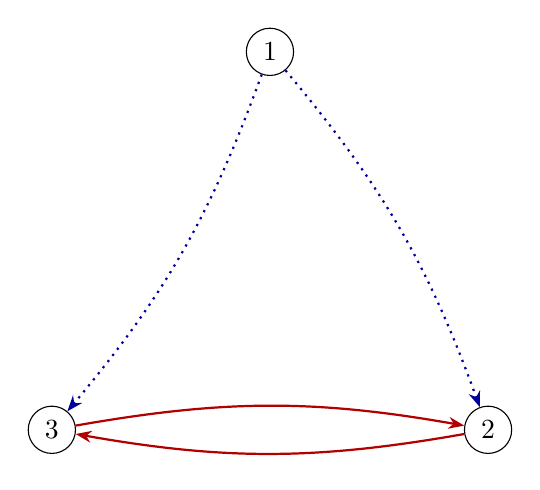
\begin{tikzpicture}[>={Stealth[length=2mm]}]
\node[draw,circle,minimum size=6mm,inner sep=0pt] (n0) at (0.00,3.20) {1};
\node[draw,circle,minimum size=6mm,inner sep=0pt] (n1) at (2.77,-1.60) {2};
\node[draw,circle,minimum size=6mm,inner sep=0pt] (n2) at (-2.77,-1.60) {3};
\draw[->,red!70!black,thick] (n1) to[bend left=10] (n2);
\draw[->,red!70!black,thick] (n2) to[bend left=10] (n1);
\draw[->,blue!60!black,thick,dotted] (n0) to[bend left=10] (n1);
\draw[->,blue!60!black,thick,dotted] (n0) to[bend left=10] (n2);
\end{tikzpicture}
\end{center}
\noindent Solid: defeats. Dashed: supports. Dotted: one party's case is part of another's.
\begin{enumerate}
\item The texts: the Spirit sent by the Son and named for him
\item From the Father and the Son (Aquinas; Florence; Westminster)
\item From the Father alone (Photius; Ware)
\end{enumerate}
\begin{longtable}{@{}>{\raggedright\arraybackslash}p{0.3\textwidth} >{\raggedright\arraybackslash}p{0.3\textwidth} >{\raggedright\arraybackslash}p{0.3\textwidth}@{}}
\toprule
\textbf{From} & \textbf{To} & \textbf{Edge} \\
\midrule
\endhead
2 \emph{From the Father and the Son (Aquinas; Florence; Westminster)} & 3 \emph{From the Father alone (Photius; Ware)} & defeats \\
3 \emph{From the Father alone (Photius; Ware)} & 2 \emph{From the Father and the Son (Aquinas; Florence; Westminster)} & defeats \\
1 \emph{The texts: the Spirit sent by the Son and named for him} & 2 \emph{From the Father and the Son (Aquinas; Florence; Westminster)} & is part of \\
1 \emph{The texts: the Spirit sent by the Son and named for him} & 3 \emph{From the Father alone (Photius; Ware)} & is part of \\
\bottomrule
\end{longtable}
\noindent The defeats are the cells of \texttt{procession\allowbreak{}Dispute\_\allowbreak{}defeats}, the supports the cells of \texttt{procession\allowbreak{}Dispute\_\allowbreak{}supports} and the parts the cells of \texttt{procession\allowbreak{}Dispute\_\allowbreak{}part\allowbreak{}Of}, each computed from the parties' premises and checked by the kernel. The attacks derived through support and through parts are reported, not counted: every verdict is computed from the defeats alone. Every derived attack is already a defeat.
\par\medskip\noindent\textbf{\texttt{lst\_\allowbreak{}stands\_\allowbreak{}with\_\allowbreak{}the\_\allowbreak{}west}}\par\nobreak\noindent
\textbf{LST stands with the West}: one reading satisfies both, the Western reading.

{\small\begin{verbatim}
theorem lst_stands_with_the_west : processionDispute.StandTogether [Party.lst,
    Party.western]
-- axioms: propext, Classical.choice, Quot.sound
\end{verbatim}}
\par\medskip\noindent\textbf{\texttt{lst\_\allowbreak{}stands\_\allowbreak{}with\_\allowbreak{}the\_\allowbreak{}east}}\par\nobreak\noindent
\textbf{LST stands with the East} too: the Eastern reading satisfies both. So LST’s position takes no side, which is what it says of itself.

{\small\begin{verbatim}
theorem lst_stands_with_the_east : processionDispute.StandTogether [Party.lst,
    Party.eastern]
-- axioms: propext, Classical.choice, Quot.sound
\end{verbatim}}
\paragraph*{What the dispute decides}
\leavevmode\par\nobreak
\par\medskip\noindent\textbf{\texttt{texts\allowbreak{}Unanswered}}\par\nobreak\noindent
How far the dispute is settled, in one stage. Nothing defeats LST, so it comes first, and nothing joins it: the West has the East for a defeater, the East has the West, and LST answers neither.

\paragraph{What the dispute forces is exactly \emph{The texts: the Spirit sent by the Son and named for him}.}
\begin{itemize}
\item Stage 1: \emph{The texts: the Spirit sent by the Son and named for him}.
\begin{itemize}
\item \emph{The texts: the Spirit sent by the Son and named for him} is defeated by nothing.
\end{itemize}
\item Nothing else is forced:
\begin{itemize}
\item \emph{From the Father alone (Photius; Ware)} defeats \emph{From the Father and the Son (Aquinas; Florence; Westminster)}, and nothing forced defeats \emph{From the Father alone (Photius; Ware)}.
\item \emph{From the Father and the Son (Aquinas; Florence; Westminster)} defeats \emph{From the Father alone (Photius; Ware)}, and nothing forced defeats \emph{From the Father and the Son (Aquinas; Florence; Westminster)}.
\end{itemize}
\end{itemize}
\par\noindent\textbf{What this rests on.} The reasons state 2 defeats and 5 absences of defeat, each a cell of the defeat table, \texttt{procession\allowbreak{}Dispute\_\allowbreak{}defeats}, computed from the two parties' premises and checked by the kernel. Whether an attack survives turns on the attacker's weakest link and on the rating of what it attacks, so a changed rating can change the verdict. The weakest links:
\begin{itemize}
\item \emph{The texts: the Spirit sent by the Son and named for him}, weakest at \emph{well supported}:
\begin{itemize}
\item an inference step --- \cite[3, The Triune God]{kibbey-living-systematic-theology-2026}; \cite{photius-mystagogy-1987}; \cite[178]{vischer-spirit-of-god-1981}; \cite[I, q. 36, a. 2]{aquinas-summa-1920}
\end{itemize}
\item \emph{From the Father and the Son (Aquinas; Florence; Westminster)}, weakest at \emph{disputed}:
\begin{itemize}
\item In John 16:14 what the Spirit takes from the Son is his being, not only his word --- \cite[I, q. 36, a. 2]{aquinas-summa-1920}
\item The Son’s sending of the Spirit rests on an eternal relation of Spirit to Son --- \cite[I, q. 36, a. 2]{aquinas-summa-1920}; \cite[165]{vischer-spirit-of-god-1981}
\item The divine persons are distinguished only by opposed relations of origin --- \cite[I, q. 36, a. 2]{aquinas-summa-1920}
\item an inference step --- \cite[I, q. 36, a. 2]{aquinas-summa-1920}; \cite{photius-mystagogy-1987}
\item an inference step --- \cite[165--169]{vischer-spirit-of-god-1981}; \cite[144]{vischer-spirit-of-god-1981}; \cite[183--184]{vischer-spirit-of-god-1981}; \cite[I, q. 43, a. 8]{aquinas-summa-1920}
\end{itemize}
\item \emph{From the Father alone (Photius; Ware)}, weakest at \emph{disputed}:
\begin{itemize}
\item John 15:26 “proceeds” speaks of the Spirit’s eternal origin, not only of mission --- \cite[I, q. 36, a. 2]{aquinas-summa-1920}; \cite{photius-mystagogy-1987}
\item In John 15:26 Jesus names the Spirit’s source, the Father, and no other --- \cite{photius-mystagogy-1987}; \cite{ware-orthodox-church-1993}
\item The Father is the one cause of the Son and of the Spirit --- \cite{photius-mystagogy-1987}; \cite{ware-orthodox-church-1993}
\item an inference step --- \cite{photius-mystagogy-1987}; \cite[I, q. 36, a. 2]{aquinas-summa-1920}
\item an inference step --- \cite[Florence, Session 6 (1439), Laetentur caeli]{tanner-decrees-1990}; \cite{pcpcu-greek-latin-traditions-1995}; \cite{photius-mystagogy-1987}
\end{itemize}
\end{itemize}
\par\medskip\noindent\textbf{\texttt{the\_\allowbreak{}texts\_\allowbreak{}prevail}}\par\nobreak\noindent
\textbf{What the texts establish prevails, and nothing more.} What the dispute forces before any choice between rivals is exactly LST’s position: the Spirit is related to the Son as well as to the Father. Nothing defeats it, because the West and the East both hold every premise it holds.

What this does not claim: that the Filioque is false, or that it is true. The West and the East are in a standoff, and neither is forced.

{\small\begin{verbatim}
theorem the_texts_prevail : Framework.grounded processionDispute.defeats =
    Solver.toSet [Party.lst]
-- axioms: propext, Classical.choice, Quot.sound
\end{verbatim}}
\par\medskip\noindent\textbf{\texttt{western\allowbreak{}With\allowbreak{}The\allowbreak{}Texts}}\par\nobreak\noindent
Why the West can be defended: with LST, it answers the East itself.

\paragraph{\emph{From the Father and the Son (Aquinas; Florence; Westminster)} is accepted on some resolution.}
\begin{itemize}
\item A position holding \emph{The texts: the Spirit sent by the Son and named for him}, \emph{From the Father and the Son (Aquinas; Florence; Westminster)} can be held.
\item None of \emph{The texts: the Spirit sent by the Son and named for him}, \emph{From the Father and the Son (Aquinas; Florence; Westminster)} defeats another, and each attack on them is answered from among them:
\begin{itemize}
\item \emph{From the Father alone (Photius; Ware)} defeats \emph{From the Father and the Son (Aquinas; Florence; Westminster)}, and \emph{From the Father and the Son (Aquinas; Florence; Westminster)} defeats \emph{From the Father alone (Photius; Ware)}.
\end{itemize}
\end{itemize}
\par\noindent\textbf{What this rests on.} The reasons state 2 defeats and 5 absences of defeat, each a cell of the defeat table, \texttt{procession\allowbreak{}Dispute\_\allowbreak{}defeats}, computed from the two parties' premises and checked by the kernel. Whether an attack survives turns on the attacker's weakest link and on the rating of what it attacks, so a changed rating can change the verdict. The weakest links:
\begin{itemize}
\item \emph{The texts: the Spirit sent by the Son and named for him}, weakest at \emph{well supported}:
\begin{itemize}
\item an inference step --- \cite[3, The Triune God]{kibbey-living-systematic-theology-2026}; \cite{photius-mystagogy-1987}; \cite[178]{vischer-spirit-of-god-1981}; \cite[I, q. 36, a. 2]{aquinas-summa-1920}
\end{itemize}
\item \emph{From the Father and the Son (Aquinas; Florence; Westminster)}, weakest at \emph{disputed}:
\begin{itemize}
\item In John 16:14 what the Spirit takes from the Son is his being, not only his word --- \cite[I, q. 36, a. 2]{aquinas-summa-1920}
\item The Son’s sending of the Spirit rests on an eternal relation of Spirit to Son --- \cite[I, q. 36, a. 2]{aquinas-summa-1920}; \cite[165]{vischer-spirit-of-god-1981}
\item The divine persons are distinguished only by opposed relations of origin --- \cite[I, q. 36, a. 2]{aquinas-summa-1920}
\item an inference step --- \cite[I, q. 36, a. 2]{aquinas-summa-1920}; \cite{photius-mystagogy-1987}
\item an inference step --- \cite[165--169]{vischer-spirit-of-god-1981}; \cite[144]{vischer-spirit-of-god-1981}; \cite[183--184]{vischer-spirit-of-god-1981}; \cite[I, q. 43, a. 8]{aquinas-summa-1920}
\end{itemize}
\item \emph{From the Father alone (Photius; Ware)}, weakest at \emph{disputed}:
\begin{itemize}
\item John 15:26 “proceeds” speaks of the Spirit’s eternal origin, not only of mission --- \cite[I, q. 36, a. 2]{aquinas-summa-1920}; \cite{photius-mystagogy-1987}
\item In John 15:26 Jesus names the Spirit’s source, the Father, and no other --- \cite{photius-mystagogy-1987}; \cite{ware-orthodox-church-1993}
\item The Father is the one cause of the Son and of the Spirit --- \cite{photius-mystagogy-1987}; \cite{ware-orthodox-church-1993}
\item an inference step --- \cite{photius-mystagogy-1987}; \cite[I, q. 36, a. 2]{aquinas-summa-1920}
\item an inference step --- \cite[Florence, Session 6 (1439), Laetentur caeli]{tanner-decrees-1990}; \cite{pcpcu-greek-latin-traditions-1995}; \cite{photius-mystagogy-1987}
\end{itemize}
\end{itemize}
\par\medskip\noindent\textbf{\texttt{western\_\allowbreak{}defensible}}\par\nobreak\noindent
\textbf{The Western position can be defended}, together with LST’s: some maximal defensible position, one no other party can join without losing that, holds both.

{\small\begin{verbatim}
theorem western_defensible : Framework.CredulouslyAccepted
    processionDispute.defeats Party.western
-- axioms: propext, Classical.choice, Quot.sound
\end{verbatim}}
\par\medskip\noindent\textbf{\texttt{western\allowbreak{}Answered\allowbreak{}By\allowbreak{}The\allowbreak{}East}}\par\nobreak\noindent
Why the West is not forced: a defensible position holds the East, and the East defeats the West.

\paragraph{\emph{From the Father and the Son (Aquinas; Florence; Westminster)} is not accepted on every resolution.}
\begin{itemize}
\item A position holding \emph{The texts: the Spirit sent by the Son and named for him}, \emph{From the Father alone (Photius; Ware)} can be held, and it holds \emph{From the Father alone (Photius; Ware)}; \emph{From the Father alone (Photius; Ware)} conflicts with \emph{From the Father and the Son (Aquinas; Florence; Westminster)}: \emph{From the Father alone (Photius; Ware)} defeats \emph{From the Father and the Son (Aquinas; Florence; Westminster)}, and \emph{From the Father and the Son (Aquinas; Florence; Westminster)} defeats \emph{From the Father alone (Photius; Ware)}.
\item None of \emph{The texts: the Spirit sent by the Son and named for him}, \emph{From the Father alone (Photius; Ware)} defeats another, and each attack on them is answered from among them:
\begin{itemize}
\item \emph{From the Father and the Son (Aquinas; Florence; Westminster)} defeats \emph{From the Father alone (Photius; Ware)}, and \emph{From the Father alone (Photius; Ware)} defeats \emph{From the Father and the Son (Aquinas; Florence; Westminster)}.
\end{itemize}
\end{itemize}
\par\noindent\textbf{What this rests on.} The reasons state 2 defeats and 5 absences of defeat, each a cell of the defeat table, \texttt{procession\allowbreak{}Dispute\_\allowbreak{}defeats}, computed from the two parties' premises and checked by the kernel. Whether an attack survives turns on the attacker's weakest link and on the rating of what it attacks, so a changed rating can change the verdict. The weakest links:
\begin{itemize}
\item \emph{From the Father alone (Photius; Ware)}, weakest at \emph{disputed}:
\begin{itemize}
\item John 15:26 “proceeds” speaks of the Spirit’s eternal origin, not only of mission --- \cite[I, q. 36, a. 2]{aquinas-summa-1920}; \cite{photius-mystagogy-1987}
\item In John 15:26 Jesus names the Spirit’s source, the Father, and no other --- \cite{photius-mystagogy-1987}; \cite{ware-orthodox-church-1993}
\item The Father is the one cause of the Son and of the Spirit --- \cite{photius-mystagogy-1987}; \cite{ware-orthodox-church-1993}
\item an inference step --- \cite{photius-mystagogy-1987}; \cite[I, q. 36, a. 2]{aquinas-summa-1920}
\item an inference step --- \cite[Florence, Session 6 (1439), Laetentur caeli]{tanner-decrees-1990}; \cite{pcpcu-greek-latin-traditions-1995}; \cite{photius-mystagogy-1987}
\end{itemize}
\item \emph{From the Father and the Son (Aquinas; Florence; Westminster)}, weakest at \emph{disputed}:
\begin{itemize}
\item In John 16:14 what the Spirit takes from the Son is his being, not only his word --- \cite[I, q. 36, a. 2]{aquinas-summa-1920}
\item The Son’s sending of the Spirit rests on an eternal relation of Spirit to Son --- \cite[I, q. 36, a. 2]{aquinas-summa-1920}; \cite[165]{vischer-spirit-of-god-1981}
\item The divine persons are distinguished only by opposed relations of origin --- \cite[I, q. 36, a. 2]{aquinas-summa-1920}
\item an inference step --- \cite[I, q. 36, a. 2]{aquinas-summa-1920}; \cite{photius-mystagogy-1987}
\item an inference step --- \cite[165--169]{vischer-spirit-of-god-1981}; \cite[144]{vischer-spirit-of-god-1981}; \cite[183--184]{vischer-spirit-of-god-1981}; \cite[I, q. 43, a. 8]{aquinas-summa-1920}
\end{itemize}
\item \emph{The texts: the Spirit sent by the Son and named for him}, weakest at \emph{well supported}:
\begin{itemize}
\item an inference step --- \cite[3, The Triune God]{kibbey-living-systematic-theology-2026}; \cite{photius-mystagogy-1987}; \cite[178]{vischer-spirit-of-god-1981}; \cite[I, q. 36, a. 2]{aquinas-summa-1920}
\end{itemize}
\end{itemize}
\par\medskip\noindent\textbf{\texttt{western\_\allowbreak{}not\_\allowbreak{}forced}}\par\nobreak\noindent
\textbf{Nor is it forced.} A maximal defensible position holds LST’s position and the East’s, and cannot hold the West’s with them.

{\small\begin{verbatim}
theorem western_not_forced : ¬Framework.SkepticallyAccepted
    processionDispute.defeats Party.western
-- axioms: propext, Classical.choice, Quot.sound
\end{verbatim}}
\par\medskip\noindent\textbf{\texttt{eastern\allowbreak{}With\allowbreak{}The\allowbreak{}Texts}}\par\nobreak\noindent
Why the East can be defended: with LST, it answers the West itself.

\paragraph{\emph{From the Father alone (Photius; Ware)} is accepted on some resolution.}
\begin{itemize}
\item A position holding \emph{The texts: the Spirit sent by the Son and named for him}, \emph{From the Father alone (Photius; Ware)} can be held.
\item None of \emph{The texts: the Spirit sent by the Son and named for him}, \emph{From the Father alone (Photius; Ware)} defeats another, and each attack on them is answered from among them:
\begin{itemize}
\item \emph{From the Father and the Son (Aquinas; Florence; Westminster)} defeats \emph{From the Father alone (Photius; Ware)}, and \emph{From the Father alone (Photius; Ware)} defeats \emph{From the Father and the Son (Aquinas; Florence; Westminster)}.
\end{itemize}
\end{itemize}
\par\noindent\textbf{What this rests on.} The reasons state 2 defeats and 5 absences of defeat, each a cell of the defeat table, \texttt{procession\allowbreak{}Dispute\_\allowbreak{}defeats}, computed from the two parties' premises and checked by the kernel. Whether an attack survives turns on the attacker's weakest link and on the rating of what it attacks, so a changed rating can change the verdict. The weakest links:
\begin{itemize}
\item \emph{The texts: the Spirit sent by the Son and named for him}, weakest at \emph{well supported}:
\begin{itemize}
\item an inference step --- \cite[3, The Triune God]{kibbey-living-systematic-theology-2026}; \cite{photius-mystagogy-1987}; \cite[178]{vischer-spirit-of-god-1981}; \cite[I, q. 36, a. 2]{aquinas-summa-1920}
\end{itemize}
\item \emph{From the Father alone (Photius; Ware)}, weakest at \emph{disputed}:
\begin{itemize}
\item John 15:26 “proceeds” speaks of the Spirit’s eternal origin, not only of mission --- \cite[I, q. 36, a. 2]{aquinas-summa-1920}; \cite{photius-mystagogy-1987}
\item In John 15:26 Jesus names the Spirit’s source, the Father, and no other --- \cite{photius-mystagogy-1987}; \cite{ware-orthodox-church-1993}
\item The Father is the one cause of the Son and of the Spirit --- \cite{photius-mystagogy-1987}; \cite{ware-orthodox-church-1993}
\item an inference step --- \cite{photius-mystagogy-1987}; \cite[I, q. 36, a. 2]{aquinas-summa-1920}
\item an inference step --- \cite[Florence, Session 6 (1439), Laetentur caeli]{tanner-decrees-1990}; \cite{pcpcu-greek-latin-traditions-1995}; \cite{photius-mystagogy-1987}
\end{itemize}
\item \emph{From the Father and the Son (Aquinas; Florence; Westminster)}, weakest at \emph{disputed}:
\begin{itemize}
\item In John 16:14 what the Spirit takes from the Son is his being, not only his word --- \cite[I, q. 36, a. 2]{aquinas-summa-1920}
\item The Son’s sending of the Spirit rests on an eternal relation of Spirit to Son --- \cite[I, q. 36, a. 2]{aquinas-summa-1920}; \cite[165]{vischer-spirit-of-god-1981}
\item The divine persons are distinguished only by opposed relations of origin --- \cite[I, q. 36, a. 2]{aquinas-summa-1920}
\item an inference step --- \cite[I, q. 36, a. 2]{aquinas-summa-1920}; \cite{photius-mystagogy-1987}
\item an inference step --- \cite[165--169]{vischer-spirit-of-god-1981}; \cite[144]{vischer-spirit-of-god-1981}; \cite[183--184]{vischer-spirit-of-god-1981}; \cite[I, q. 43, a. 8]{aquinas-summa-1920}
\end{itemize}
\end{itemize}
\par\medskip\noindent\textbf{\texttt{eastern\_\allowbreak{}defensible}}\par\nobreak\noindent
\textbf{The Eastern position can be defended}, together with LST’s.

{\small\begin{verbatim}
theorem eastern_defensible : Framework.CredulouslyAccepted
    processionDispute.defeats Party.eastern
-- axioms: propext, Classical.choice, Quot.sound
\end{verbatim}}
\par\medskip\noindent\textbf{\texttt{eastern\allowbreak{}Answered\allowbreak{}By\allowbreak{}The\allowbreak{}West}}\par\nobreak\noindent
Why the East is not forced: a defensible position holds the West, and the West defeats the East.

\paragraph{\emph{From the Father alone (Photius; Ware)} is not accepted on every resolution.}
\begin{itemize}
\item A position holding \emph{The texts: the Spirit sent by the Son and named for him}, \emph{From the Father and the Son (Aquinas; Florence; Westminster)} can be held, and it holds \emph{From the Father and the Son (Aquinas; Florence; Westminster)}; \emph{From the Father and the Son (Aquinas; Florence; Westminster)} conflicts with \emph{From the Father alone (Photius; Ware)}: \emph{From the Father and the Son (Aquinas; Florence; Westminster)} defeats \emph{From the Father alone (Photius; Ware)}, and \emph{From the Father alone (Photius; Ware)} defeats \emph{From the Father and the Son (Aquinas; Florence; Westminster)}.
\item None of \emph{The texts: the Spirit sent by the Son and named for him}, \emph{From the Father and the Son (Aquinas; Florence; Westminster)} defeats another, and each attack on them is answered from among them:
\begin{itemize}
\item \emph{From the Father alone (Photius; Ware)} defeats \emph{From the Father and the Son (Aquinas; Florence; Westminster)}, and \emph{From the Father and the Son (Aquinas; Florence; Westminster)} defeats \emph{From the Father alone (Photius; Ware)}.
\end{itemize}
\end{itemize}
\par\noindent\textbf{What this rests on.} The reasons state 2 defeats and 5 absences of defeat, each a cell of the defeat table, \texttt{procession\allowbreak{}Dispute\_\allowbreak{}defeats}, computed from the two parties' premises and checked by the kernel. Whether an attack survives turns on the attacker's weakest link and on the rating of what it attacks, so a changed rating can change the verdict. The weakest links:
\begin{itemize}
\item \emph{From the Father and the Son (Aquinas; Florence; Westminster)}, weakest at \emph{disputed}:
\begin{itemize}
\item In John 16:14 what the Spirit takes from the Son is his being, not only his word --- \cite[I, q. 36, a. 2]{aquinas-summa-1920}
\item The Son’s sending of the Spirit rests on an eternal relation of Spirit to Son --- \cite[I, q. 36, a. 2]{aquinas-summa-1920}; \cite[165]{vischer-spirit-of-god-1981}
\item The divine persons are distinguished only by opposed relations of origin --- \cite[I, q. 36, a. 2]{aquinas-summa-1920}
\item an inference step --- \cite[I, q. 36, a. 2]{aquinas-summa-1920}; \cite{photius-mystagogy-1987}
\item an inference step --- \cite[165--169]{vischer-spirit-of-god-1981}; \cite[144]{vischer-spirit-of-god-1981}; \cite[183--184]{vischer-spirit-of-god-1981}; \cite[I, q. 43, a. 8]{aquinas-summa-1920}
\end{itemize}
\item \emph{From the Father alone (Photius; Ware)}, weakest at \emph{disputed}:
\begin{itemize}
\item John 15:26 “proceeds” speaks of the Spirit’s eternal origin, not only of mission --- \cite[I, q. 36, a. 2]{aquinas-summa-1920}; \cite{photius-mystagogy-1987}
\item In John 15:26 Jesus names the Spirit’s source, the Father, and no other --- \cite{photius-mystagogy-1987}; \cite{ware-orthodox-church-1993}
\item The Father is the one cause of the Son and of the Spirit --- \cite{photius-mystagogy-1987}; \cite{ware-orthodox-church-1993}
\item an inference step --- \cite{photius-mystagogy-1987}; \cite[I, q. 36, a. 2]{aquinas-summa-1920}
\item an inference step --- \cite[Florence, Session 6 (1439), Laetentur caeli]{tanner-decrees-1990}; \cite{pcpcu-greek-latin-traditions-1995}; \cite{photius-mystagogy-1987}
\end{itemize}
\item \emph{The texts: the Spirit sent by the Son and named for him}, weakest at \emph{well supported}:
\begin{itemize}
\item an inference step --- \cite[3, The Triune God]{kibbey-living-systematic-theology-2026}; \cite{photius-mystagogy-1987}; \cite[178]{vischer-spirit-of-god-1981}; \cite[I, q. 36, a. 2]{aquinas-summa-1920}
\end{itemize}
\end{itemize}
\par\medskip\noindent\textbf{\texttt{eastern\_\allowbreak{}not\_\allowbreak{}forced}}\par\nobreak\noindent
\textbf{Nor is it forced.} A maximal defensible position holds LST’s position and the West’s, and cannot hold the East’s with them.

{\small\begin{verbatim}
theorem eastern_not_forced : ¬Framework.SkepticallyAccepted
    processionDispute.defeats Party.eastern
-- axioms: propext, Classical.choice, Quot.sound
\end{verbatim}}
\subsection*{Appendix: the claims and their sources}
\addcontentsline{toc}{subsection}{Appendix: the claims and their sources}
The texts every party reads, the readings each party gives them, and the conclusion that divides them. The texts are kept apart from the readings, so that a reader can see which claims are what John, Paul and Luke say, and which are what a tradition says they mean.

\subsubsection*{Citation and classification for every atom}
Every claim must name a source, or the encoding will not build (\texttt{cite}). Each reading is cited to a source that holds it. Each step’s rating is cited to a reader who accepts the claims it starts from (its grounds) and still denies where it ends, or says that no such reader was found after a search for one.

\subsubsection*{The claims, numbered}
\begin{longtable}{@{}r >{\raggedright\arraybackslash}p{0.30\textwidth} l >{\raggedright\arraybackslash}p{0.19\textwidth} >{\raggedright\arraybackslash}p{0.21\textwidth}@{}}
\toprule
 & claim & kind & held & source \\
\midrule
\endhead
\pvartarget{TestimonyArguments.Trinity}{1}$P_{1}$ & John 15:26 — the Spirit of truth, who proceeds from the Father\textsuperscript{\dag} & textual & Christian, hist.-gramm., consensus & John 15:26 \\
\pvartarget{TestimonyArguments.Trinity}{2}$P_{2}$ & John 15:26; 16:7 — the Son sends the Spirit, from the Father\textsuperscript{\dag} & textual & Christian, hist.-gramm., consensus & John 15:26; John 16:7 \\
\pvartarget{TestimonyArguments.Trinity}{3}$P_{3}$ & Galatians 4:6; Romans 8:9 — the Spirit of his Son, the Spirit of Christ\textsuperscript{\dag} & textual & Christian, hist.-gramm., consensus & Gal 4:6; Rom 8:9 \\
\pvartarget{TestimonyArguments.Trinity}{4}$P_{4}$ & Acts 2:33 — the exalted Son receives the promised Spirit and pours him out\textsuperscript{\dag} & textual & Christian, hist.-gramm., consensus & Acts 2:33 \\
\pvartarget{TestimonyArguments.Trinity}{5}$P_{5}$ & John 16:14 — the Spirit will take what is the Son’s and declare it\textsuperscript{\dag} & textual & Christian, hist.-gramm., consensus & John 16:14 \\
\pvartarget{TestimonyArguments.Trinity}{6}$P_{6}$ & The Spirit is related to the Son as well as to the Father & theological & Christian, hist.-gramm., well supported & \cite[3, The Triune God]{kibbey-living-systematic-theology-2026}; \cite{photius-mystagogy-1987}; \cite[I, q. 36, a. 2]{aquinas-summa-1920} \\
\pvartarget{TestimonyArguments.Trinity}{7}$P_{7}$ & In John 16:14 what the Spirit takes from the Son is his being, not only his word & interpretive & Roman Catholic, disputed & \cite[I, q. 36, a. 2]{aquinas-summa-1920} \\
\pvartarget{TestimonyArguments.Trinity}{8}$P_{8}$ & The Son’s sending of the Spirit rests on an eternal relation of Spirit to Son & theological & Roman Catholic, disputed & \cite[I, q. 36, a. 2]{aquinas-summa-1920}; \cite[165]{vischer-spirit-of-god-1981} \\
\pvartarget{TestimonyArguments.Trinity}{9}$P_{9}$ & John 14:16 — the Son and the Spirit are two persons: “another Helper” & theological & Christian, hist.-gramm., well supported & John 14:16; \cite[3, The Triune God]{kibbey-living-systematic-theology-2026} \\
\pvartarget{TestimonyArguments.Trinity}{10}$P_{10}$ & The divine persons are distinguished only by opposed relations of origin & theological & Roman Catholic, disputed & \cite[I, q. 36, a. 2]{aquinas-summa-1920} \\
\pvartarget{TestimonyArguments.Trinity}{11}$P_{11}$ & The Son is not from the Spirit: “which no one says” & theological & Roman Catholic, well supported & \cite[I, q. 36, a. 2]{aquinas-summa-1920} \\
\pvartarget{TestimonyArguments.Trinity}{12}$P_{12}$ & John 15:26 “proceeds” speaks of the Spirit’s eternal origin, not only of mission & interpretive & Christian, hist.-gramm., disputed & \cite[I, q. 36, a. 2]{aquinas-summa-1920}; \cite{photius-mystagogy-1987} \\
\pvartarget{TestimonyArguments.Trinity}{13}$P_{13}$ & In John 15:26 Jesus names the Spirit’s source, the Father, and no other & interpretive & Eastern Orthodox, disputed & \cite{photius-mystagogy-1987}; \cite{ware-orthodox-church-1993} \\
\pvartarget{TestimonyArguments.Trinity}{14}$P_{14}$ & The Father is the one cause of the Son and of the Spirit & theological & Eastern Orthodox, disputed & \cite{photius-mystagogy-1987}; \cite{ware-orthodox-church-1993} \\
\pvartarget{TestimonyArguments.Trinity}{15}$P_{15}$ & The Spirit proceeds eternally from the Father and the Son & theological & Roman Catholic, disputed & \cite[Florence, Session 6 (1439), Laetentur caeli]{tanner-decrees-1990}; \cite[II.3]{westminster-confession-1647} \\
\pvartarget{TestimonyArguments.Trinity}{16}$P_{16}$ & John 5:19, 30 — the Son does nothing of his own accord, but the sender’s will\textsuperscript{\dag} & textual & Christian, hist.-gramm., consensus & John 5:19; John 5:30 \\
\pvartarget{TestimonyArguments.Trinity}{17}$P_{17}$ & John 14:28 — “the Father is greater than I”\textsuperscript{\dag} & textual & Christian, hist.-gramm., consensus & John 14:28 \\
\pvartarget{TestimonyArguments.Trinity}{18}$P_{18}$ & John 20:17 — the risen Jesus: “my God and your God”\textsuperscript{\dag} & textual & Christian, hist.-gramm., consensus & John 20:17 \\
\pvartarget{TestimonyArguments.Trinity}{19}$P_{19}$ & 1 Corinthians 11:3 — “the head of Christ is God”\textsuperscript{\dag} & textual & Christian, hist.-gramm., consensus & 1 Cor 11:3 \\
\pvartarget{TestimonyArguments.Trinity}{20}$P_{20}$ & 1 Corinthians 15:28 — “the Son himself will also be subjected to him”\textsuperscript{\dag} & textual & Christian, hist.-gramm., consensus & 1 Cor 15:28 \\
\pvartarget{TestimonyArguments.Trinity}{21}$P_{21}$ & Philippians 2:6 — “though he was in the form of God”\textsuperscript{\dag} & textual & Christian, hist.-gramm., consensus & Phil 2:6 \\
\pvartarget{TestimonyArguments.Trinity}{22}$P_{22}$ & There is a real order of Father and Son in the work of salvation & theological & Christian, hist.-gramm., well supported & \cite[3, The Triune God]{kibbey-living-systematic-theology-2026} \\
\pvartarget{TestimonyArguments.Trinity}{23}$P_{23}$ & In John 14:28 “greater” means the Son is less in his divinity & interpretive & Christian, hist.-gramm., disputed & \cite[De Synodis 28]{schaff-nicene-post-nicene-fathers-2-4-1892}; \cite[On the Trinity I.7.14]{schaff-nicene-post-nicene-fathers-1-3-1887}; \cite[102]{calvin-commentary-john-2-1847} \\
\pvartarget{TestimonyArguments.Trinity}{24}$P_{24}$ & In John 14:28 the Son is less in the form of a servant, not in the form of God & interpretive & Christian, hist.-gramm., disputed & \cite[On the Trinity I.7.14]{schaff-nicene-post-nicene-fathers-1-3-1887} \\
\pvartarget{TestimonyArguments.Trinity}{25}$P_{25}$ & The Father is “greater” as the one the Son is begotten from & interpretive & Christian, hist.-gramm., disputed & \cite[Against the Arians I.13.58]{schaff-nicene-post-nicene-fathers-2-4-1892} \\
\pvartarget{TestimonyArguments.Trinity}{26}$P_{26}$ & In John 14:28 Christ compares his humbled state as Mediator with his glory & interpretive & Reformed Protestant, disputed & \cite[102--103]{calvin-commentary-john-2-1847} \\
\pvartarget{TestimonyArguments.Trinity}{27}$P_{27}$ & The sending and obeying are the outworking of an eternal authority and submission & theological & Christian, hist.-gramm., disputed & \cite[40]{grudem-doctrinal-deviations-2015}; \cite{grudem-ets-trinity-2016}; \cite{ware-father-son-holy-spirit-2005} \\
\pvartarget{TestimonyArguments.Trinity}{28}$P_{28}$ & The Son is equal to the Father in power: “of one substance, power, and eternity” & theological & Reformed Protestant, well supported & \cite[II.3]{westminster-confession-1647} \\
\pvartarget{TestimonyArguments.Trinity}{29}$P_{29}$ & Eternal subordination in authority would deny the Son’s equality in power & theological & Christian, hist.-gramm., disputed & \cite[323]{giles-ets-trinity-2008}; \cite{giles-jesus-and-the-father-2006} \\
\pvartarget{TestimonyArguments.Trinity}{30}$P_{30}$ & The Son is less than the Father in his divinity & theological & Christian, hist.-gramm., disputed & \cite[Theodoret, Ecclesiastical History I.4]{schaff-nicene-post-nicene-fathers-2-3-1892} \\
\pvartarget{TestimonyArguments.Trinity}{31}$P_{31}$ & There is an eternal relationship of authority and submission of Father and Son & theological & Christian, hist.-gramm., disputed & \cite{grudem-ets-trinity-2016}; \cite{ware-father-son-holy-spirit-2005} \\
\bottomrule
\end{longtable}

\noindent\footnotesize \textsuperscript{\dag} grounded in scripture alone: the reading is assumed, not argued for.
\normalsize
\subsubsection*{How this is checked}
\par\medskip\noindent\textbf{\texttt{lst\allowbreak{}On\allowbreak{}The\allowbreak{}Triune\allowbreak{}God}}\par\nobreak\noindent
LST §3, “The Triune God”. The renderer adds the section sign.

{\small\begin{verbatim}
def lstOnTheTriuneGod : Bib.Locus :=
  Bib.Locus.sectionRef "3, The Triune God"
\end{verbatim}}
\par\medskip\noindent\textbf{\texttt{aquinas\allowbreak{}On\allowbreak{}The\allowbreak{}Son}}\par\nobreak\noindent
Aquinas on whether the Spirit proceeds from the Son.

{\small\begin{verbatim}
def aquinasOnTheSon : Bib.Locus :=
  Bib.Locus.sectionRef "I, q. 36, a. 2"
\end{verbatim}}
\par\medskip\noindent\textbf{\texttt{florence\allowbreak{}On\allowbreak{}The\allowbreak{}Procession}}\par\nobreak\noindent
Florence’s definition of the procession.

{\small\begin{verbatim}
def florenceOnTheProcession : Bib.Locus :=
  Bib.Locus.sectionRef "Florence, Session 6 (1439), Laetentur caeli"
\end{verbatim}}
\paragraph*{Ratings for inference steps}
\leavevmode\par\nobreak
\par\medskip\noindent\textbf{\texttt{on\allowbreak{}The\allowbreak{}Relation}}\par\nobreak\noindent
\textbf{The step from the texts to a relation between the Spirit and the Son is well supported.} LST draws it: the texts “establish a real relation of the Spirit to both Father and Son”. It was audited for a reader who grants the texts and denies that the Spirit is related to the Son, and none was found. The Eastern readers affirm the relation in their own terms. Photius grants that the Spirit is the “Spirit of His Son” (Galatians 4:6), “because He is in the Son” and of one substance with him. Staniloae writes that “in the East, it is not denied that at the origin of the sending of the Spirit by the Son there is a special eternal relationship between the Son and the Spirit”. What they deny is that the relation is one of origin, and the claim the step delivers does not say that it is.

{\small\begin{verbatim}
def onTheRelation : Source :=
  {
    primary :=
      Reference.work kibbeyLivingSystematicTheology lstOnTheTriuneGod,
    supporting :=
      [Reference.work photiusMystagogy,
        Reference.work vischerSpiritOfGod (Bib.Locus.page 178),
        Reference.work aquinasSumma aquinasOnTheSon],
    tradition := Tradition.christianHistoricalGrammatical,
    confidence := Confidence.wellSupported }
\end{verbatim}}
\par\medskip\noindent\textbf{\texttt{on\allowbreak{}The\allowbreak{}Receiving}}\par\nobreak\noindent
\textbf{The step from John 16:14 is rated \texttt{disputed}, conservatively.} Aquinas holds it (reply to objection 1). The Eastern readers reject its conclusion by denying a ground: that what the Spirit takes from the Son is his being, and not what he declares. No reader was sought who grants that ground and still denies the Filioque, so the step is not rated above the bottom.

{\small\begin{verbatim}
def onTheReceiving : Source :=
  { primary := Reference.work aquinasSumma aquinasOnTheSon,
    supporting := [Reference.work photiusMystagogy],
    tradition := Tradition.romanCatholic, confidence := Confidence.disputed }
\end{verbatim}}
\par\medskip\noindent\textbf{\texttt{on\allowbreak{}The\allowbreak{}Mission}}\par\nobreak\noindent
\textbf{The step from mission to origin is disputed.} Its grounds are that the Son sends the Spirit, that the Spirit is named for him, and that the sending rests on an eternal relation of the Spirit to the Son. Three readers grant all three and deny that the Spirit is from the Son. Moltmann holds that “there must be an inner-trinitarian basis for the temporal sending of the Spirit through Christ”, and that the Spirit “receives from the Father his own perfect divine existence (hypostasis), and obtains from the Son his relational form”. Bobrinskoy speaks of the Spirit “resting on the Son from all eternity”. Staniloae, following Gregory of Cyprus: “though the Spirit’s manifestation is by the Son, his coming into existence is not by the Son”. Aquinas reaches origin from the relation because “there cannot be in God any relations opposed to each other, except relations of origin” (I, q. 36, a. 2). He does not hold that every sending shows origin: a person sent proceeds from the sender when the sender is “designated as the principle of the person sent” (I, q. 43, a. 8).

{\small\begin{verbatim}
def onTheMission : Source :=
  { primary := Reference.work vischerSpiritOfGod (Bib.Locus.pages 165 169),
    supporting :=
      [Reference.work vischerSpiritOfGod (Bib.Locus.page 144),
        Reference.work vischerSpiritOfGod (Bib.Locus.pages 183 184),
        Reference.work aquinasSumma (Bib.Locus.sectionRef "I, q. 43, a. 8")],
    tradition := Tradition.easternOrthodox, confidence := Confidence.disputed }
\end{verbatim}}
\par\medskip\noindent\textbf{\texttt{on\allowbreak{}The\allowbreak{}Opposition}}\par\nobreak\noindent
\textbf{The step from distinction is well supported, once its unstated premise is written in.} Aquinas argues that “if He were not from Him, He could in no wise be personally distinguished from Him”, because the persons are distinguished “only by the relations” and only opposed relations distinguish. It was audited for a reader who grants that, and that the Son is not from the Spirit, and still denies the Filioque, and none was found. Its rejecters deny a ground. Scotus denies that only opposed relations distinguish: a relation, he says, “distinguishes not only from the opposite relation but also from any disparate relation” (\emph{Ordinatio} I, d. 11, q. 2), though he holds the Filioque on other grounds. Gregory of Nazianzus names each person by “the very fact of being Unbegotten or Begotten, or Proceeding” (\emph{Oration} 31.9), which distinguishes the Son and the Spirit by their relations to the Father. Neither Scotus nor Gregory is yet in this library’s bibliography, so the rating cites Aquinas alone.

{\small\begin{verbatim}
def onTheOpposition : Source :=
  { primary := Reference.work aquinasSumma aquinasOnTheSon,
    tradition := Tradition.romanCatholic,
    confidence := Confidence.wellSupported }
\end{verbatim}}
\par\medskip\noindent\textbf{\texttt{on\allowbreak{}The\allowbreak{}Words}}\par\nobreak\noindent
\textbf{The Eastern step from John 15:26 is rated \texttt{disputed}, conservatively.} Photius holds it. The Western readers reject its conclusion by denying a ground: that the verse, naming the Father, names the whole of the Spirit’s source. Augustine asks why the Son said “he proceeds from the Father”, and answers, “so as not to imply, He proceeds not from me” (\emph{Tractates on John} 99.8): he grants the verse and denies that it excludes the Son. The step has not been audited for a reader who grants that ground and still holds the Filioque, as the Western step from distinction was; until it is, it stays at the bottom.

{\small\begin{verbatim}
def onTheWords : Source :=
  { primary := Reference.work photiusMystagogy,
    supporting := [Reference.work aquinasSumma aquinasOnTheSon],
    tradition := Tradition.easternOrthodox, confidence := Confidence.disputed }
\end{verbatim}}
\par\medskip\noindent\textbf{\texttt{on\allowbreak{}The\allowbreak{}Monarchy}}\par\nobreak\noindent
\textbf{The Eastern step from the monarchy is disputed.} Florence denies its ground as it stands: the Father is “the source and principle of all deity”, but the Spirit “has his essence and his subsistent being from the Father together with the Son”, and the Greek fathers’ “through the Son” signifies the Son “as cause”. The Pontifical Council for Promoting Christian Unity (1995) grants the ground almost word for word, the Father “the sole Trinitarian Cause (Aitia) or principle (principium) of the Son and the Holy Spirit”, and still confesses the Father, “with the Son, the single principle from which the Spirit proceeds”. It does so by distinguishing two senses of “proceed”: the Greek ἐκπόρευσις, origin from the Father alone, and the Latin \emph{processio}, which may be from the Son.

{\small\begin{verbatim}
def onTheMonarchy : Source :=
  { primary := Reference.work tannerDecrees florenceOnTheProcession,
    supporting :=
      [Reference.work pcpcuGreekAndLatinTraditions,
        Reference.work photiusMystagogy],
    tradition := Tradition.romanCatholic, confidence := Confidence.disputed }
\end{verbatim}}
\paragraph*{The order texts}
\leavevmode\par\nobreak
\par\medskip\noindent\textbf{\texttt{augustine\allowbreak{}On\allowbreak{}John14}}\par\nobreak\noindent
Augustine on John 14:28.

{\small\begin{verbatim}
def augustineOnJohn14 : Bib.Locus :=
  Bib.Locus.sectionRef "On the Trinity I.7.14"
\end{verbatim}}
\par\medskip\noindent\textbf{\texttt{athanasius\allowbreak{}On\allowbreak{}John14}}\par\nobreak\noindent
Athanasius on John 14:28.

{\small\begin{verbatim}
def athanasiusOnJohn14 : Bib.Locus :=
  Bib.Locus.sectionRef "Against the Arians I.13.58"
\end{verbatim}}
\paragraph*{Ratings for the steps over the order texts}
\leavevmode\par\nobreak
\par\medskip\noindent\textbf{\texttt{on\allowbreak{}The\allowbreak{}Order}}\par\nobreak\noindent
\textbf{The step from the order texts to a real order is well supported.} LST draws it: the texts “establish real personal and mediatorial order”. It was audited for a reader who grants the texts and denies the order, and none was found. The nearest is the Oneness writer David Bernard (\emph{The Oneness of God}, 1983, ch. 8), who grants every text, and the sending, the obedience and the final subjection, and reads “Father” and “Son” as the deity and the humanity of one person: “The flesh was subject to the Spirit.” The order as stated here does not say whether Father and Son are two persons, so he grants it too. That they are is LST’s next question.

{\small\begin{verbatim}
def onTheOrder : Source :=
  {
    primary :=
      Reference.work kibbeyLivingSystematicTheology lstOnTheTriuneGod,
    tradition := Tradition.christianHistoricalGrammatical,
    confidence := Confidence.wellSupported }
\end{verbatim}}
\par\medskip\noindent\textbf{\texttt{on\allowbreak{}The\allowbreak{}Arian\allowbreak{}Reading}}\par\nobreak\noindent
\textbf{The Arian step is well supported}: the reading it starts from already says the Son is less in divinity, and no reader was found who grants the reading and denies that. The dissent is from the reading, which is rated \texttt{disputed}.

{\small\begin{verbatim}
def onTheArianReading : Source :=
  { primary := Reference.work npnf1v3 augustineOnJohn14,
    supporting :=
      [Reference.work calvinJohn2 (Bib.Locus.page 102),
        Reference.work npnf2v3
          (Bib.Locus.sectionRef "Theodoret, Ecclesiastical History I.4")],
    tradition := Tradition.christianHistoricalGrammatical,
    confidence := Confidence.wellSupported }
\end{verbatim}}
\par\medskip\noindent\textbf{\texttt{on\allowbreak{}The\allowbreak{}Two\allowbreak{}Forms}}\par\nobreak\noindent
\textbf{Augustine’s step is well supported}: his reading already says the Son is equal in the form of God, and no reader was found who grants it and holds him less in divinity. Gregory of Nazianzus grants the reading: “to say that he is greater than the Son considered as man, is true indeed, but is no great thing” (\emph{Oration} 30.7).

{\small\begin{verbatim}
def onTheTwoForms : Source :=
  { primary := Reference.work npnf1v3 augustineOnJohn14,
    supporting :=
      [Reference.work npnfCyrilGregory
          (Bib.Locus.sectionRef "Gregory of Nazianzus, Oration 30.7")],
    tradition := Tradition.christianHistoricalGrammatical,
    confidence := Confidence.wellSupported }
\end{verbatim}}
\par\medskip\noindent\textbf{\texttt{on\allowbreak{}The\allowbreak{}Begetter}}\par\nobreak\noindent
\textbf{Athanasius’s step is well supported, because his reading says “not in greatness”.} Readers who grant only that the Father is greater as the one the Son is from, and still hold him greater in divinity, deny that clause. The creed of Sirmium (357) says the Father is “greater in honour and dignity and Godhead, and in the very name of Father, the Son Himself testifying, ‘The Father that sent Me is greater than I’” (Athanasius, \emph{De Synodis} 28). Gregory of Nazianzus reports opponents who, granting that “in respect of being the Cause the Father is greater than the Son”, “deduce the conclusion that He is greater by Nature also”, and calls the inference a fallacy (\emph{Oration} 29.15). So the dispute sits in the reading, which is rated \texttt{disputed}.

{\small\begin{verbatim}
def onTheBegetter : Source :=
  { primary := Reference.work npnf2v4 athanasiusOnJohn14,
    supporting :=
      [Reference.work npnf2v4 (Bib.Locus.sectionRef "De Synodis 28"),
        Reference.work npnfCyrilGregory
          (Bib.Locus.sectionRef "Gregory of Nazianzus, Oration 29.15")],
    tradition := Tradition.christianHistoricalGrammatical,
    confidence := Confidence.wellSupported }
\end{verbatim}}
\par\medskip\noindent\textbf{\texttt{on\allowbreak{}The\allowbreak{}Mediators\allowbreak{}State}}\par\nobreak\noindent
\textbf{Calvin’s step is well supported}: no reader was found who grants that the verse compares the Mediator’s humbled state with his glory and holds that it says the Son is less in divinity.

{\small\begin{verbatim}
def onTheMediatorsState : Source :=
  { primary := Reference.work calvinJohn2 (Bib.Locus.pages 102 103),
    tradition := Tradition.reformedProtestant,
    confidence := Confidence.wellSupported }
\end{verbatim}}
\par\medskip\noindent\textbf{\texttt{on\allowbreak{}Calvin\allowbreak{}Against\allowbreak{}The\allowbreak{}Fathers}}\par\nobreak\noindent
\textbf{Calvin against the Fathers’ reply}: reading the verse of the Mediator’s state, he denies that it speaks of the Son’s human nature, and calls the Fathers’ reply “neither correct nor appropriate”. Rated \texttt{well\allowbreak{}Supported}: his reading says that the comparison is of states, not natures, and no reader was found who grants that and reads the verse of the human nature.

{\small\begin{verbatim}
def onCalvinAgainstTheFathers : Source :=
  { primary := Reference.work calvinJohn2 (Bib.Locus.page 102),
    tradition := Tradition.reformedProtestant,
    confidence := Confidence.wellSupported }
\end{verbatim}}
\par\medskip\noindent\textbf{\texttt{on\allowbreak{}The\allowbreak{}Eternal\allowbreak{}Order}}\par\nobreak\noindent
\textbf{The step from the order to an eternal order of authority is well supported}: its reading already says the order is the outworking of an eternal relationship, and no reader was found who grants that and denies the relationship. The dissent is from the reading. Augustine grants the order and reads it otherwise: the Son “was not sent in virtue of some disparity of power or substance … but in virtue of the Son being from the Father” (\emph{On the Trinity} IV.20.27, as Grudem quotes it, 2016).

{\small\begin{verbatim}
def onTheEternalOrder : Source :=
  { primary := Reference.work grudemDoctrinalDeviations (Bib.Locus.page 40),
    supporting :=
      [Reference.work grudemEts2016, Reference.work wareFatherSonSpirit],
    tradition := Tradition.christianHistoricalGrammatical,
    confidence := Confidence.wellSupported }
\end{verbatim}}
\par\medskip\noindent\textbf{\texttt{on\allowbreak{}Equal\allowbreak{}Power}}\par\nobreak\noindent
\textbf{Giles’s step is well supported}: no reader was found who grants both its grounds and still affirms an eternal submission. Grudem grants the first, the Son’s equality in power: the Evangelical Theological Society, of which he was president, confesses the persons “equal in power and glory”, and he “zealously” guards “against greater ontological power” for the Father (2016, I.A.4). He denies the second, that eternal submission would deny that equality. Giles concedes that the second is his reading: “I cannot see how anyone could distinguish these terms” (2008, p. 327). So the dispute sits in the reading, which is rated \texttt{disputed}.

{\small\begin{verbatim}
def onEqualPower : Source :=
  { primary := Reference.work gilesEtsTrinity (Bib.Locus.page 327),
    supporting :=
      [Reference.work gilesJesusAndTheFather, Reference.work grudemEts2016],
    tradition := Tradition.christianHistoricalGrammatical,
    confidence := Confidence.wellSupported }
\end{verbatim}}
\paragraph*{Citations}
\leavevmode\par\nobreak
\par\medskip\noindent\textbf{\texttt{cite}}\par\nobreak\noindent
Citation and classification for every atom. Total, so nothing is uncited.

{\small\begin{verbatim}
def cite : Claim → AtomMeta
\end{verbatim}}

\bibliographystyle{plain}
\bibliography{references}
\end{document}
